%
% This template has been created by:
% Pascal Bercher, pascal.bercher@anu.edu.au
%
% This is version 1.01 (13. Sep 2022)
%
% version history:
% - 1.00 (3. Dec 2021)  - first version that deserves a version number! :)
% - 1.01 (13. Sep 2022) - fixed wrong TOC link to Bibliography
%
% Make sure to use the newest version available on git!
%
% I was too lazy to put it under a specific license, but you are still free to use and alter it.
% But since I put a *lot* of effort (and experience)



\documentclass[a4paper,twoside,cleardoublepage=plain,bibliography=totoc]{scrbook}

\usepackage[a4paper]{geometry}                    % used for defining the title page


\usepackage{xurl}                                 % allows long URLs to break at any position
\usepackage[backref=page]{hyperref}               % defines style of references / links
\hypersetup{
linktocpage,                                      % in the table of contents, the numbers serve as links, not the entries
colorlinks  = true,                               % the items are colored instead of colored boxes around them
urlcolor    = cyan,
linkcolor   = red,
citecolor   = blue
}
% the following makes back references more appealing.
% Taken from: https://tex.stackexchange.com/questions/183702/formatting-back-references-in-bibliography-bibtex
\renewcommand*{\backref}[1]{}
\renewcommand*{\backrefalt}[4]{[%
\ifcase #1 Not cited.%
  \or Cited on page~#2.%
  \else Cited on pages #2.%
\fi]}




\usepackage{datetime}                             % to be able to print month & year on title page
  \newdateformat{monthonly}{\monthname[\THEMONTH]}
\usepackage{amssymb,amsthm,amsmath}               % standard math packages; often used
\usepackage{graphicx}                             % allows including graphics
\usepackage{natbib}                               % a specific citation style

\setcitestyle{numbers}
\setcitestyle{square}

\usepackage{floatrow}                             % allows to place a caption next to a figure
  \floatsetup[table]{capposition=top}             %  forces table captions to appear on top.
\usepackage{booktabs}                             % for tables that actually look nice!
\usepackage{paralist}                             % provides compactitem, a more compact itemize
\usepackage{titlesec}                             % used to add those horizontal lines around chapter package; see defs below.
\usepackage[standardsections]{scrhack}            %  fixes an error causes by loading titlesec for class scrbook
\usepackage{parskip}                              % when this is included, no indentations are used for new paragraphs,
                                                  % and instead paragraphs are separated by a small distance between them
\usepackage{tikz}
\usetikzlibrary{shapes,arrows}  
\usepackage{tikz-cd}
\usepackage{holtexbasic}
\usepackage{enumitem}


\renewcommand{\HOLConst}[1]{{\textsf{\upshape\small #1}}}
\renewcommand{\HOLTyOp}[1]{\mbox{\fontencoding{T1}\fontfamily{bch}\fontseries{m}\fontshape{it}\fontsize{9.5}{10}\selectfont #1}}
\renewcommand{\HOLinline}[1]{\ensuremath{#1}}
\newcommand{\holthmenv}[1]{\begin{array}[t]{l}#1\end{array}}
\renewcommand{\HOLKeyword}[1]{\texttt{#1}}

\newenvironment{holmath}{\begin{displaymath}\begin{array}{l}}{\end{array}\end{displaymath}\ignorespacesafterend}
\newenvironment{holarray}{\begin{array}[t]{l}}{\end{array}}


% [requires titlesec]
% Surrounds all chapter titles by lines,
\titleformat{\chapter}[display]
{\bfseries\huge}
{\filleft\Large\chaptertitlename~\thechapter}
{3ex}
{\titlerule\vspace{1.5ex}\filright}
[\vspace{1ex}\titlerule]

% fixes a compilation errror that otherwise occurs in combination with scrbook
% see https://tex.stackexchange.com/questions/625083/adding-horizontal-line-before-and-after-chapter-heading-in-scrbook
% \titleformat{\section}
%  {\normalfont\Large\bfseries}{\thesection}{1em}{}
% \titleformat{\subsection}
%  {\normalfont\large\bfseries}{\thesubsection}{1em}{}
% \titleformat{\subsubsection}
%  {\normalfont\normalsize\bfseries}{\thesubsubsection}{1em}{}
 

 

% Set your individual data for the title page in the configuration file
% AND DONT SCREW UP THIS DATA! You should know, for example, whether it's
% an Honours thesis or not, or in which semester it is running.

% Set your name:
%  (Well, your name.)
\newcommand{\AuthorName} {Ratmir Mugattarov}


% Set the title of your work:
%  (Choose an informative and interesting title.)
\newcommand{\ProjectTitle} {Election Verification with HOL4 and CakeML}


% Set which titlepage layout you prefer. Both provide the exact same
% information, they only differ in design to give you a bit of individuality
%  (change second line accordingly)
\newif\ifStandardTitle % do not delete this part!
\StandardTitletrue     % comment out (or use \StandardTitlefalse)
                       % to switch to an alternative title page layout


% Set the name of your school:
%  (School of Computing, School of Engineering,
%   or School of Cybernetics)
\newcommand{\School} {School of Computing}


% Set the name of your college:
%  (However your College is called.)
\newcommand{\College} {College of Engineering, Computing and Cybernetics (CECC)}


% Set your project points:
%  (6 or 12 or 24)
\newcommand{\ProjectPoints} {24}


% Set whether it's an Honours thesis:
%  (change second line accordingly)
\newif\ifHonoursThesis % do not delete this part!
\HonoursThesistrue     % or \HonoursThesisfalse or comment out


% Set your semester:
%  (S1 or S2 or S1/S2 or S2/S1 or Summer)
\newcommand{\Semester} {S2/S1}


% Set your year:
%  (YYYY or YYYY--YYYY in case of S2/S1)
\newcommand{\Year} {2022--2023}


% Set your degree:
%  (Whatever your degree is called.)
%  (Only required if Honours = true)
\newcommand{\Degree} {Bachelor of Science (Honours)}


% Set your course code and name:
%  (Whatever your course code and name is.)
%  (Only required if Honours = false)
\newcommand{\CourseCode} {COMP4540}
\newcommand{\CourseName} {Software Engineering Research Project}


% Set name of first supervisor:
%   (Whatever her or his name is.)
\newcommand{\FirstSupervisor} {Dr.\ Thomas Haines}


% Set whether there's a second supervisor:
%  (change second line accordingly)
\newif\ifTwoSupervisors % do not delete this part!
\TwoSupervisorstrue     % or \TwoSupervisorsfalse or comment out


% Set name of second supervisor:
%  (Whatever her or his name is.)
%  (Only required if TwoSupervisors = true)
\newcommand{\SecondSupervisor} {%
\\Prof.\ Dr.\ Michael Norrish
}
                             % to specify data used in the title page

% define your own macros here

\newcommand{\Eff} {\ensuremath{\mathit{eff}}}  % example command without arguments
\newcommand{\Pre} {\ensuremath{\mathit{pre}}}  % (again)

% Note that you can easily specify arguments:
% \newcommand{\someMacro}[2] {Argument 1: #1, Argument 2: #2} % example command with two arguments
% you use it via \someMacro{Hello}{World!}


% the following commands are being provided by the amsthm package
% the first parameter states the new environmet's name that can be
% used (due to this definition here) and the second the name that
% will appear in the PDF document
\theoremstyle{definition}
\newtheorem{definition}{Definition}   % well, a formal definition!
\theoremstyle{plain}
\newtheorem{prop}{Proposition} % like a theorem, but less important or evolved
\newtheorem{lem}{Lemma}        % used within a proof of a theorem
\newtheorem{thm}{Theorem}      % well, a theorem! :) important and evolved
\newtheorem{cor}{Corollary}    % basically either a proposition or theorem,
                               %  but one that follows from another theorem.
% There's a lot you can configure about the appearance. If interested,
% open the manual of amsthm or google for tutorials etc. on that package

% the following add a symbol to the definition environment to make it more
% clear when a definition ends (as there is no difference in fonts!). From:
% https://tex.stackexchange.com/questions/226334/change-a-amsthm-theorem-ending
\newcommand{\xqed}[1]{%
    \leavevmode\unskip\penalty9999 \hbox{}\nobreak\hfill
    \quad\hbox{\ensuremath{#1}}}
\newcommand{\Endofdef}{\xqed{\blacksquare}}
\newenvironment{defn}[1]{%
    \begin{definition}#1}{%
    \Endofdef\end{definition}%
}
                                    % define all your macros here


\begin{document}

\pagenumbering{roman}

%
% This document contains two different definitions of the title page
% which one is chosen is defined in the file configutation.tex
%


% only the title page is centered; all other pages are aligned according to books
\newgeometry{left=2.5cm,right=2.5cm,top=2.5cm}
\thispagestyle{empty}

\newdateformat{monthyeardate}{%
  \monthname[\THEMONTH] \THEYEAR}


\ifStandardTitle % the first style is defined now

\noindent
\begin{minipage}[t]{6cm}%
{\footnotesize%
\raisebox{-\height}{{\bfseries The Australian National University}} \\
~2600 ACT~\textbar~Canberra~\textbar~Australia}
\end{minipage}%
\hfill%
\begin{minipage}[b]{10cm}%
\hfill\raisebox{-\height}{
\includegraphics[height=2 cm]{figures/ANU-logos/ANU_Primary_Horizontal_Black.jpg}}
\end{minipage}


\ \\[2em]
\phantom{x} \hfill
\begin{minipage}{58.75 mm}
\raggedright
\bfseries \School\\[.5em]
\mdseries%
\noindent\College
\end{minipage}\\[6 em]
\hfill

\noindent
\parbox{140mm}{\sffamily \bfseries \Huge %
\ProjectTitle%
}\\[.75 em]
{--- \ProjectPoints{} pt \ifHonoursThesis Honours \else research \fi project (\Semester{} \Year)}\\[3 em]


\ifHonoursThesis%
A thesis submitted for the degree\\
\emph{\Degree}\\[3 em]
\else%
A report submitted for the course\\
\emph{\CourseCode, \CourseName}\\[3 em]
\fi




\noindent
{\footnotesize \textbf{By:}}\\
\AuthorName\\[2em]



\noindent
{\footnotesize \bfseries Supervisor\ifTwoSupervisors{}s\fi:}\\
{\footnotesize \FirstSupervisor%
\ifTwoSupervisors\\\SecondSupervisor\fi}\\[2 em]
\vfill
{\footnotesize \monthyeardate\today}



\else % the alternative design of the title page



\begin{center}
\ \\[1em]
{\bfseries \Huge \ProjectTitle}\\[4em]
%
\ifHonoursThesis%
\Large{A thesis submitted for the degree}\\
\Large{\emph{\Degree}}\\[.5em]
{\ProjectPoints{} pt Honours project, \Semester{} \Year}
\else%
\Large{A report submitted for the course}\\
\Large{\emph{\CourseCode, \CourseName}}\\[.5em]
{\ProjectPoints{} pt research project, \Semester{} \Year}
\fi
%
\ \\[4em]
{\footnotesize \textbf By:}\\
\textbf{\AuthorName}\\[3em]
%
{\bfseries Supervisor\ifTwoSupervisors{}s\fi:}\\
{\FirstSupervisor%
\ifTwoSupervisors\\\SecondSupervisor\fi}\\[6em]
%

\includegraphics[height=2.5cm]{figures/ANU-logos/ANU_Primary_Horizontal_Black.jpg}\ \\[3em]
%
{\bfseries \School}\\
{\mdseries \College}\\
The Australian National University
%
\vfill
\normalsize{\monthyeardate\today}
\end{center}



\fi


\restoregeometry
                               % define your title page
{\sffamily\bfseries\Large Declaration:}\\

I declare that this work:\\

\begin{itemize}
  \item upholds the principles of academic integrity, as defined in the \href{https://www.anu.edu.au/about/governance/legislation}{University Academic Misconduct Rules};
  \item is original, except where collaboration (for example group work) has been authorised in writing by the course convener in the class summary and/or Wattle site;
  \item is produced for the purposes of this assessment task and has not been submitted for assessment in any other context, except where authorised in writing by the course convener;
  \item gives appropriate acknowledgement of the ideas, scholarship and intellectual property of others insofar as these have been used;
  \item in no part involves copying, cheating, collusion, fabrication, plagiarism or recycling.
\end{itemize}


\vspace{1 cm}
\hfill \the\year\ \monthname, \AuthorName
\newpage


% The current requirements can be found on:
% https://policies.anu.edu.au/ppl/document/ANUP_004603  (section 18) -- date: 9.2.2022
                             % includes the declaration of authorship
\chapter*{Acknowledgements}
I would like to express my sincere gratitude to Thomas Haines for his support and advice during this project. I am extremely grateful to Michael Norrish, who generously spent time with me explaining the specifics of HOL and CakeML during numerous live coding sessions. Special thanks to Hing-Lun (Joseph) Chan, who developed the Abstract Algebra Library, which our project extensively relies on. Many thanks to the whole Co-Lab team, especially to Jan Shaddock and ANU for facilitating the whole process and providing such a great research experience. I would also like to thank everyone on the CakeML contributors Slack channel for their helpful insights and support.
                        % optional acknowledgements
\chapter*{Abstract}
Elections are a crucial part of democracy. However, traditional paper-based voting systems are laborious and lack transparency. Electronic elections promise improvement through automation, but also present challenges due to the error-prone nature of software. These complexities amplify with the integration of cryptography, potentially leading to additional errors. Even minor errors can have significant consequences, such as the wrong candidate winning an election.

In response to these challenges, we advocate for error-free electronic elections. As a solution, we propose the development of an election verifier program, a tool designed to verify the integrity of electronic elections. This work presents an improved technique to develop such a verifier, leading to better trustworthiness of electronic elections.                                % your abstract
% \chapter*{Notations}
HOL \\
ZKP \\
$\mathbb{N}$\\
$\mathbb{Z}$\\
                               % notations
% \input{0-definitions}                             % definitions

% table of contents (nothing to do for you)
\renewcommand{\contentsname}{Table of Contents}   % would otherwise just be "Contents",
\cleardoublepage\tableofcontents\cleardoublepage  % which might sound less nice
\pagenumbering{arabic}

% actual report content
\chapter{Introduction}\label{chap:introduction}
\section{Election}
The election process is a critical component of democracy. 
However, traditional paper voting faces numerous challenges. 
Voting and tallying are labor-intensive, the vote counting process is not 
transparent, audit is not available for the general public, and the process 
does not scale well. As society advances rapidly, our democratic processes must 
adapt to meet new demands. Electronic voting provides the benefits of automation 
and online access; however, it introduces its own set of problems. Since electronic 
voting relies on software, it inherently contains errors, which can be difficult to 
eliminate entirely \cite{brooks1975mythical}. Fixing one issue often introduces another. 
Numerous instances of errors in electronic voting have been 
documented \cite{ChangFong2016TheCS, Halderman2015TheNS, Haines2022RunningTR}. 
Such errors undermine public trust in the electoral process. Given the importance 
of elections, we cannot tolerate more than zero errors in the election process. 
Therefore, if we want to employ electronic voting, it is crucial to provide a 
zero-error guarantee in electronic voting software for it to be considered both 
reliable and trustworthy.
\section{Software} 
To ensure an error-free election, it is vital to provide the same guarantee 
for the software conducting the voting. Software errors are common, mainly 
because the development process inherently doesn't guarantee correctness. 
Historically, there is a gap \label{gap} between the theoretical correctness 
and the actual operation of the software. The industry standard for ensuring 
operational correctness is through testing, but this method only identifies 
existing errors and cannot assure their complete absence. A more effective, 
though less frequently used, method is a formal proof of the program code or 
algorithm. Regrettably, this proof is often conducted separately from the compiled 
code, either on paper or within a proof assistant environment, resulting in a gap 
between theory and practice. This separation occurs largely due to two 
factors: (1) programming languages are not typically designed for proof 
writing; (2) compilers, which have been found to contain 
errors \cite{Yang2011FindingAU}, are not purposed to maintain code 
correctness. Therefore, software industry is not yet mature enough 
to satisfy high requirements for electronic election.
\section{Cryptography}
Electronic election employ cryptography to protect the process and 
information from unauthorised intervention. The use of cryptography 
in electronic voting systems introduces an additional source of complexity, 
thereby increasing the potential for errors. The cryptographic techniques 
employed in these systems are based on sigma protocol technology and abstract 
algebra theories. Given their non-trivial nature, even a minor mistake could 
significantly compromise an election. There are well-documented 
cases \cite{Halderman2015TheNS, Springall2014SecurityAO, Haines2022RunningTR}, where 
cryptographic errors have resulted in exploitable vulnerabilities in electronic election. 
For example, a minor flaw could enable an election official to covertly alter votes, as 
demonstrated in a case involving the SwissVote 
election 
system\footnote{https://www.unimelb.edu.au/newsroom/news/2019/march/researchers-find-trapdoor-in-swissvote-election-system}. 
The combination of complexity of cryptographic techniques and the inherent difficulty 
in ensuring software accuracy makes the task of implementing error-free electronic voting exceedingly challenging.
\section{Election Verification} 
Electronic voting has the potential to enhance democratic elections, 
but the trustworthiness of electronic voting is currently in question 
due to inability to guarantee absence of errors. There is a partial solution to this problem. 

Electronic elections perform  cryptographic computation producing encrypted data. This data can be used to 
verify computation posterior to the election and guarantee certain properties of election to hold. The 
verification program, functioning independently once the election is completed, is smaller and less 
complex than the electronic election system, as it isolates properties and does no interaction. Less 
complex programs of smaller sizes are typically less susceptible to errors, consequently providing a 
greater degree of certainty in their absence. 

In order to be able to rely on such verification we can formally prove that the code of this small 
verifying program has no errors and does what it supposed to do, however, as discussed earlier, the 
environment where we develop the proof and compiler are also computer programs containing errors. 
There is no guarantee that such errors do not propagate cause election with errors be positively verified.
\section{Problem} 
As discussed above, ensuring that the required properties of electronic elections are met is an 
extremely challenging task. However, this is a crucial requirement for electronic elections to be 
considered trustworthy. The goal of our research is to improve the current situation by addressing 
these challenges.
\section{Solution}
A potential solution to this problem is to use such proof environment and compiler that guarantee 
to produce valid proofs and correctly operating executable program, to develop election verification 
program that is guaranteed to have no errors. Then, employ such verification programs to verify required properties of electronic election one by one. Using such approach all required properties of electronic election can be guaranteed. This process can ensure that a given election is error-free.

Unfortunately, the above conceptual approach is not widely practiced, possibly due to lack of 
information and detailed guidelines to follow. The solution we propose is a generalised 
technique that demonstrate an example for how to develop such  election verification program 
for some selected properties of electronic election and use it to verify election to guarantee that electronic election comply with some target property. Our proposed technique will help developers to rely on the above concept and guarantee certain properties of electronic election to hold.
\section{Contribution}
Our contribution is an improvement to the previously developed similar 
technique \cite{Haines2019VerifiableHT}. A particular improvement that we make, 
is joining the gap in correctness of election verification program from the code 
to the operational program. We achieve it by employing (1) a theorem proof environment 
that is verified to accept only valid poofs, and (2) a compiler that is guaranteed to 
produce executable program which behaves precisely as it code specifies. 
                            % introduction
\chapter{Background}


\section{Overview}
\begin{itemize}
\item \textbf{Tools} that we discuss are used to develop proven correct software. Proof assistants, such as HOL4, can be used to write mathematical proofs about the code, and help verifying the correctness of election software. CakeML is a programming language that can be used to compile correctly operating programs.

\item \textbf{Algebra} is used to understand the underlying mathematics of cryptography. Abelian groups, fields, cyclic groups, and discrete logarithms are all important concepts in cryptography.

\item \textbf{Cryptography} is used to protect electronic elections. Zero knowledge proofs, sigma protocols, and the Schnorr protocol and other are all cryptographic techniques that are useful for electronic elections.

\item \textbf{Electronic Elections} are the application of cryptography and other technologies to the voting process. Helios Voting is an example of an electronic election system. The IACR 2022 Director Election conducted with Helios is an example of a real election that we use for our project.
\end{itemize}

These concepts are all interconnected. Proof assistants are used to verify the correctness of election related software, which is written in a verified programming  language like CakeML. Algebra essentials, such as groups and fields, are used to understand the underlying mathematics of cryptography. Cryptography is used to secure electronic elections, which are deployed via systems like Helios Voting. 


\section{Tools}
\subsection{Proof Assistants}

A proof assistant is a software tool, akin to a programming language, specifically designed for writing and structuring mathematical proofs. While it doesn't automate the proof process entirely, a proof assistant can streamline some of the more routine, tedious tasks associated with constructing proofs.

Primarily, proof assistants offer an extensive library of standard mathematical theories and tactics. These libraries facilitate easy search of theorems by formal parameters, along with a suite of specialised tools available to proof developers. The formalisation of mathematical theories through proof assistants is a currently thriving research area within the realm of formal logic.

The objectives for constructing formal proofs can greatly vary. For instance, in mathematics, proof assistants are used to reduce labor-intensive tasks such as exhaustive case analysis. In the field of software development, proof assistants are utilised to verify certain properties of code, such as compliance with a given specification. This allows developers to simultaneously develop and prove the code according to clearly defined correctness criteria, which significantly bolsters confidence in the code's correct operation.

However, it's important to note that the use of proof assistants is not a common practice in general software development. The reason being, working with proof assistants necessitates a solid understanding of logic and mathematical proofs, thereby presenting a steep learning curve. Additionally, the requirement to develop proofs alongside the working code can result in higher labor hours. These factors contribute to a higher cost of development.

Consequently, proof-based software development is mostly employed in critical areas where the cost of a software operation error could be exceedingly high. These sectors include, but are not limited to, aerospace and cryptography.\\

It's crucial to understand that a proof of code correctness doesn't inherently ensure the correct execution of a program. As outlined in the introductory chapter, there exists a gap in software correctness. Both the compiler and the proof assistant's code need to be verified for correctness of program operation.

Notably, not all proof assistants have their own code verified, nor do they necessarily have the compiler's code verified. This state of non-verification isn't inherently problematic—it largely depends on the specific objectives of the proof assistant.

For instance, LEAN\footnote{https://leanprover.github.io} operates on the principle of peer review by numerous advanced mathematicians, with no immediate plans for formal verification of its code. On the other hand, the HOL4\footnote{https://hol-theorem-prover.org} proof assistant has undergone formal verification using an intricate self-verification technique, which will be discussed in more detail later. The distinction in approaches reflects the diverse range of applications and methodologies in the field of proof assistants.

\subsection{HOL4}
HOL4 is a proof assistant and automatic theorem prover. HOL stands for Higher Order Logic, number 4 stands for version number. This software generates an interactive proof writing environment called HOL. This name is the same as the name of area of mathematics. In this work we will use word \text{``HOL"} without version number for software and environment, and make it clear by the context which one of those we refer to. In many cases, when we have a high level discussion we do not need to differentiate them. 

Higher-order logic is a form of predicate logic that allows quantification not only over individual variables but also over function and predicate symbols. This is in contrast to first-order logic, which only allows quantification over individual variables.\\
In first-order logic, we can make statements similar to \\
"For all \textbf{x}, \textbf{P(x)}" or ``There exists an \textbf{x} such that \textbf{P(x)}", \\
where \textbf{P} is a predicate and \textbf{x} is a variable that ranges over individuals in our domain of discourse.\\
Higher-order logic extends this by allowing we to make statements similar to\\
"For all functions \textbf{f}, \textbf{P(f)}" or ``There exists a predicate \textbf{P} such that \textbf{Q(P)}", \\
where \textbf{f} is a function symbol, \textbf{P} and \textbf{Q} are predicates, and we're quantifying over all possible functions or predicates in our domain.\\
HOL employs StandardML as its internal programming language. The typical proof construction process in HOL proceeds as follows:\\
Initially, the user formulates the goal as a theorem. Subsequently, they progress incrementally, either advancing from the premise towards the conclusion, or vice versa. Each step in this process is accomplished by invoking a specific theorem or a combination thereof.\\
However, in practice, the application of theorems can vary, which necessitates the user to define a specific tactic. A tactic represents the strategy for theorem application.\\
\newpage
\subsection{HOL4 Tutorial}
To illustrate this, consider the following simple example from the official HOL tutorial \cite{HOL4interaction}. Additional explanation can be found in the description manual \cite{hol4manual}.
\begin{verbatim}
open arithmeticTheory listTheory;

Theorem less_eq_mult:
  for all n:num. n <= n * n
Proof
    Induct_on n>-
    decide_tac >-
    (asm_simp_tac bool_ss [MULT]>>
        decide_tac)
QED
\end{verbatim}

The theorem we want to prove states that for any natural number $\mathbf{n}$, $\mathbf{n}$ is less than or equal to $\mathbf{n} * \mathbf{n}$. The proof of this theorem is carried out interactively with the use of tactics. We run the code line by line. 

First, we import the required theories: arithmetic theory and list theory. Then, we set the goal to prove. We want to use induction on $\mathbf{n}$ so we apply the induction tactic in relation to variable $\mathbf{n}$.

The induction tactic transforms the goal from one to two subgoals:

\begin{itemize}
    \item Base case:  $0 \leq 0 \times 0$,
    \item Step case: $(n+1) \leq (n+1) \times (n+1)$.
\end{itemize}

Then, we apply the \texttt{decide\_tac} tactic. 
This tactic in HOL is a decision procedure tactic. A decision procedure is an algorithm that can definitively answer specific kinds of questions. In the context of a theorem prover like HOL, a decision procedure is used to determine whether certain classes of statements are true or false.
This resolves the base case. And we are left with one goal to prove step case. 

Next we apply tactics \textbf{\texttt{asm\_sim\_tac}}. This is a simplification tactic that uses both the given simpset and the current assumptions to simplify the goal.

A simpset, short for simplification set, is a collection of theorems that the simplifier uses to rewrite terms. The term \texttt{bool\_ss} in our example is a simpset that includes basic simplification rules for boolean algebra.

Simplification is a commonly used tactic in interactive theorem proving. It works by applying equalities in a way that attempts to simplify the goal, often by rewriting complex expressions into simpler ones, or even solving the goal entirely if possible.

The \texttt{asm\_simp\_tac} tactic is called with a simpset and a list of theorems, and it tries to simplify the goal by repeatedly applying these theorems, as well as the assumptions of the current goal.

So in the context of our proof, \texttt{asm\_simp\_tac bool\_ss [MULT]} is trying to simplify the goal using the theorems in \texttt{bool\_ss} and the \texttt{MULT} theorem, as well as the assumptions of the current goal.

We provide the tactic \texttt{asm\_simp\_tac} with the parameter \texttt{bool\_ss}. Additionally, we supply \texttt{bool\_ss} with a list containing a single theorem, \texttt{[MULT]}.

Where \texttt{MULT} is a theorem defined as follows:
\begin{flushleft}
\texttt{MULT = $\vdash$ ($\forall$n. 0 $\times$ n = 0) $\land$ $\forall$m n. SUC m $\times$ n = m $\times$ n + n: thm}
\end{flushleft}

\texttt{bool\_ss} refers to a simpset - a collection of theorems - that is used by the simplifier to rewrite terms. The simpset \texttt{bool\_ss} contains basic simplification rules for boolean algebra. These rules can be used by the \texttt{asm\_simp\_tac} tactic to simplify the goal during the proof process. 

In other words, \texttt{bool\_ss} provides the \texttt{asm\_simp\_tac} tactic with the rules it needs to try and simplify or solve the goal. These rules include identities and equivalences from boolean algebra that can be used to rewrite boolean expressions into simpler or equivalent forms.

Altogether, \texttt{asm\_simp\_tac bool\_ss [MULT]} is a call to the simplification tactic \texttt{asm\_simp\_tac} with the simpset \texttt{bool\_ss} and the theorems in the list \texttt{[MULT]}. 

Here, \texttt{MULT} is a theorem stating the properties of multiplication involving zero and the successor function (essentially defining how multiplication works for natural numbers in a recursive manner). It is used as an argument to the \texttt{asm\_simp\_tac} simplification tactic.

\texttt{asm\_simp\_tac bool\_ss [MULT]} instructs HOL4 to simplify the current goal using the theorems included in \texttt{bool\_ss} (which covers basic boolean algebra rules) and the multiplication theorem \texttt{MULT}. 

The simplifier will use these rules to attempt to rewrite and simplify the goal, which could involve reducing complex expressions into simpler forms or even solving the goal entirely if possible. The \texttt{asm\_simp\_tac} tactic also takes into account the current assumptions of the goal for the simplification.

Then, we again apply the \textbf{\texttt{decide\_tac}} tactic. This tactic is used to decide a goal that can be solved directly by existing facts or theorems. Applying this tactic simplifies our problem and leads us to the proof of the subgoal:

\begin{flushleft}
\textbf{\texttt{Goal proved: [.] $\vdash$ SUC n $\leq$ n $\times$ SUC n + SUC n}}
\end{flushleft}

This shows that $n+1$ is less than or equal to $n \times (n+1) + (n+1)$, which is a crucial step in our induction.

Following that, we prove the previous goal:

\begin{flushleft}
\textbf{\texttt{Goal proved: [.] $\vdash$ SUC n $\leq$ SQ(SUC n)}}
\end{flushleft}

This shows that $n+1$ is less than or equal to the square of $n+1$.

With these steps completed, we have proved our initial goal:

\begin{flushleft}
\textbf{\texttt{val it =}}\\
\textbf{\texttt{Initial goal proved: $\vdash$ $\forall$ n. n $\leq$ SQ(n): proof}}
\end{flushleft}

This confirms that for all natural numbers $n$, $n$ is less than or equal to the square of $n$.

\subsection{CakeML}
CakeML\footnote{https://cakeml.org} is a functional programming language and an ecosystem of proofs and tools built around it. It is a variant of the ML (Meta Language) family, which also includes languages such as Standard ML and OCaml. One of the distinctive features of CakeML is that it has a formally verified compiler \cite{Tan2019TheVC}, meaning that the compiler's behavior has been proven mathematically to adhere to the language's specification.

CakeML is designed with an emphasis on verifiability, robustness, and performance. It supports a range of programming constructs, including first-class functions, user-defined datatypes, pattern-matching, and mutable reference cells.

The CakeML ecosystem includes a formally verified compiler backend, a logic model of the language semantics, and a growing set of libraries and tools. The verified compiler backend provides strong guarantees about the correctness of compiled code. The logic model can be used to reason about CakeML programs within HOL4 proof assistant. The libraries and tools offer various facilities for developing and working with CakeML programs.

Currently, CakeML is an active project with ongoing research and development.

\subsection{Self-verification} 


The HOL4 theorem prover and the CakeML compiler have both been subject to rigorous formal verification processes to ensure their correctness \cite{Myreen2013StepsTV, Harrison2006TowardsSO, Abrahamsson2022CandleAV}, Result is a guarantee that HOL4 can only generate valid proofs, and that programs compiled with CakeML behave precisely as specified by their source code. This robust level of assurance is achieved through a techniques known as self-verification and self-formalisation  \cite{Kumar2016SelfFormalisationOH}. 

There is no magic here, system cannot be verified within itself as it contradicts to Goedel Second Incompleteness Theorem \cite{Gdel1966OnFU}. The trick is to ultimately reduce the initial (trusted) code base and manually verify these few lines of code. Then the rest of the code relies on this correctness.

The self-verification process employs a approach called bootstrapping and the concept of a small trusted code base, also referred to as a Trusted Code Base (TCB). This approach is fundamental to the development of both the HOL4 and CakeML systems, and is widely used in the creation of verified systems. By maintaining a small TCB and applying formal verification to the components within it, the integrity and correctness of the entire system can be assured.

HOL4 implements environment HOL. HOL4 is a theorem prover for Higher Order Logic (HOL). Its kernel, which forms the trusted code base (TCB), is written in a way that facilitates review and validation for correctness. The kernel is capable of checking proofs about more complex aspects of the system. Much of HOL4 is written in HOL itself, making it subject to verification by the HOL4 kernel.

The compiler for CakeML can be implemented as a function in is written in HOL. A proof within the HOL4 environment demonstrates that the compiler correctly follows the semantics of the CakeML language. This proof, combined with the HOL4 kernel, forms the TCB for CakeML.

Through these steps, the verification of both the HOL4 theorem prover and the CakeML compiler is achieved. This process uses a minimal TCB to ensure trust in the system, and leverages bootstrapping to build up verified layers of the system.

There is work on make it even better and give a more rigorous proof of correctness of HOL environment.
HOL is an interactive environment with its rules, properties and attributes. HOL4 implements HOL environment, but other implementations of HOL can exist. In order to prove that HOL-type environment produces only valid proofs some people implement a kernel of HOL-theorem prover using CakeML programming language \cite{Abrahamsson2022CandleAV, Kumar2014HOLWD}. This kernel of HOL theorem prover. Using bootstrapping this kernel verifies the rest of the HOL system, and implements new HOL environment. This new HOL environment is not the same HOL environment implemented by HOL4 but features the same general system parameters. 

The current state is that HOL4 correctness relies on tiny trusted code base which was thoroughly reviewed. CakeML compiler correctness relies on its implementation in HOL environment. 
There are other HOL environment that are generated by the kernel compiled by CakeML, which is implemented in (another) HOL environment. 

\section{Algebra essentials}
We used the Algebra textbook for definitions in this section\cite{Artin:1998}.

\subsection{Group}
A group is a set $\mathbf{G}$ equipped with a binary operation $\cdot$ (called the group operation) that satisfies the following axioms: \\
Closure: For all $\mathbf{g,h} \in \mathbf{G}$, $\mathbf{g} \cdot \mathbf{h} \in \mathbf{G}$. \\ 
Associativity: For all $\mathbf{g,h,k} \in \mathbf{G}$, $(\mathbf{g} \cdot \mathbf{h}) \cdot \mathbf{k} = \mathbf{g} \cdot (\mathbf{h} \cdot \mathbf{k})$. \\ 
Identity element: There exists an element $\mathbf{e} \in \mathbf{G}$ such that for all $\mathbf{g} \in \mathbf{G}$, $\mathbf{e} \cdot \mathbf{g} = \mathbf{g} \cdot \mathbf{e} = \mathbf{g}$. \\ 
Inverse element: For each $\mathbf{g} \in \mathbf{G}$, there exists an element $\mathbf{g^{-1}} \in \mathbf{G}$ \\ 
such that $\mathbf{g} \cdot \mathbf{g^{-1}} = \mathbf{g^{-1}} \cdot \mathbf{g} = \mathbf{e}$. 

\subsection{Abelian Group}
An Abelian group, also known as a commutative group, is a group $(\mathbf{G}, \cdot)$ in which the group operation is commutative, that is, for all $\mathbf{g,h} \in \mathbf{G}$, we have $\mathbf{g} \cdot \mathbf{h} = \mathbf{h} \cdot \mathbf{g}$. In other words, the order of the elements in operation does not matter.


\subsection{Field}
A field is a set $\mathbf{F}$ equipped with two binary operations, denoted by $+$ and $\cdot$, which satisfy the following axioms:

\begin{enumerate}
\item $(\mathbf{F},+)$ is an Abelian group with identity element 0, i.e., for all $\mathbf{a,b,c} \in \mathbf{F}$,
\begin{enumerate}
\item Associativity: $\mathbf{a}+( \mathbf{b}+\mathbf{c}) = (\mathbf{a}+\mathbf{b})+\mathbf{c}$.
\item Commutativity: $\mathbf{a}+\mathbf{b} = \mathbf{b}+\mathbf{a}$.
\item Identity: There exists an element 0 in $\mathbf{F}$ such that $\mathbf{a}+0 = \mathbf{a}$ for all $\mathbf{a} \in \mathbf{F}$.
\item Inverse: For every $\mathbf{a} \in \mathbf{F}$, there exists an element $-\mathbf{a} \in \mathbf{F}$ such that $\mathbf{a}+(-\mathbf{a}) = (-\mathbf{a})+\mathbf{a} = 0$.
\end{enumerate}
\item $(\mathbf{F}\setminus{0},\cdot)$ is an Abelian group with identity element 1, i.e., for all $\mathbf{a,b,c} \in \mathbf{F}\setminus{0}$,
\begin{enumerate}
\item Associativity: $\mathbf{a}\cdot (\mathbf{b}\cdot \mathbf{c}) = (\mathbf{a}\cdot \mathbf{b})\cdot \mathbf{c}$.
\item Commutativity: $\mathbf{a}\cdot \mathbf{b} = \mathbf{b}\cdot \mathbf{a}$.
\item Identity: There exists an element 1 in $\mathbf{F}\setminus{0}$ such that $\mathbf{a}\cdot 1 = \mathbf{a}$ for all $\mathbf{a} \in \mathbf{F}\setminus{0}$.
\item Inverse: For every $\mathbf{a} \in \mathbf{F}\setminus{0}$, there exists an element $\mathbf{a}^{-1} \in \mathbf{F}\setminus{0}$ such that $\mathbf{a}\cdot \mathbf{a}^{-1} = \mathbf{a}^{-1}\cdot \mathbf{a} = 1$.
\end{enumerate}
\item The distributive laws hold, i.e., for all $\mathbf{a,b,c} \in \mathbf{F}$,
\begin{enumerate}
\item Left distributivity: $\mathbf{a}\cdot(\mathbf{b}+\mathbf{c}) = \mathbf{a}\cdot \mathbf{b} + \mathbf{a}\cdot \mathbf{c}$.
\item Right distributivity: $(\mathbf{a}+\mathbf{b})\cdot \mathbf{c} = \mathbf{a}\cdot \mathbf{c} + \mathbf{b}\cdot \mathbf{c}$.
\end{enumerate}
\end{enumerate}

\subsection{Cyclic Group}
A group $(\mathbf{G}, \cdot)$ is called a cyclic group if there exists an element $\mathbf{g} \in \mathbf{G}$ such that for every element $\mathbf{x} \in \mathbf{G}$, there exists an integer $\mathbf{n}$ such that $\mathbf{x} = \mathbf{g}^\mathbf{n}$. In other words, every element of the group can be obtained by repeatedly applying the group operation to a single element, called a generator.

The order of a group $(\mathbf{G}, \cdot)$, denoted as $|\mathbf{G}|$, is the number of elements in the group. So if $\mathbf{G} = \{\mathbf{g}_1, \mathbf{g}_2, \ldots, \mathbf{g}_\mathbf{n}\}$, then $|\mathbf{G}| = \mathbf{n}$.

The order of an element $\mathbf{g} \in \mathbf{G}$, denoted as $|\mathbf{g}|$, is the smallest positive integer $\mathbf{n}$ such that $\mathbf{g}^\mathbf{n} = \mathbf{e}$, where $\mathbf{e}$ is the identity element of the group under the operation~$\cdot$. If no such positive integer $\mathbf{n}$ exists, we say that the order of $\mathbf{g}$ is infinity.

In a cyclic group generated by an element $\mathbf{g}$, the order of $\mathbf{g}$ is equal to the order of the group, i.e., $|\mathbf{g}| = |\mathbf{G}|$. This is because, by definition, we can generate every element in the group by applying the group operation to $\mathbf{g}$ some number of times.

If we have a cyclic group of prime order $\mathbf{q}$, then the set of integers modulo $\mathbf{q}$ forms a field under the operations of addition and multiplication modulo $\mathbf{q}$. This is because a prime order ensures that every non-zero element has a multiplicative inverse. The existence of additive inverses is guaranteed since we're working modulo $\mathbf{q}$. The set of integers modulo $\mathbf{q}$ is often denoted as $\mathbb{Z}_\mathbf{q}$ or $\mathbb{F}_\mathbf{q}$.

Moreover, when we're talking about a cyclic group generated by an element $\mathbf{g}$, the exponents we use to generate the group elements can be thought of as elements of this field. That is, if $\mathbf{G} = \{\mathbf{g}^0, \mathbf{g}^1, \mathbf{g}^2, ..., \mathbf{g}^{\mathbf{q}-1}\}$, then the exponents $0, 1, 2, ..., \mathbf{q}-1$ can be thought of as elements of the field $\mathbb{F}_\mathbf{q}$, since they behave like integers modulo $\mathbf{q}$ under addition and multiplication.

This connection between groups of prime order and fields is fundamental to many areas of mathematics and is particularly important in number theory and cryptography.

In modular arithmetic, an integer $\mathbf{a}$ is a quadratic residue modulo $\mathbf{n}$ if there exists an integer $\mathbf{x}$ such that the congruence $\mathbf{x}^2 \equiv \mathbf{a} \pmod{\mathbf{n}}$ holds.

The set of all quadratic residues modulo $\mathbf{n}$ is usually denoted as $(\mathbb{Z}/\mathbf{n}\mathbb{Z})^2$ or simply as $\mathbf{Q_n}$. In the special case where $\mathbf{n}$ is a prime number $\mathbf{p}$, we denote this set as $(\mathbb{Z}/\mathbf{p}\mathbb{Z})^2$~or~$\mathbf{Q_p}$.

For example, when $\mathbf{p}=5$, the quadratic residues are the numbers that are congruent to the square of some integer modulo $5$. These are $\mathbf{0}$, $\mathbf{1}$, and $\mathbf{4}$, because $0^2 \equiv 0 \pmod{5}$, $1^2 \equiv 1 \pmod{5}$, $2^2 \equiv 4 \pmod{5}$, $3^2 \equiv 4 \pmod{5}$, and $4^2 \equiv 1 \pmod{5}$.

So the set of quadratic residues modulo $5$ is $\mathbf{Q}_5 = \{{0}, {1}, {4}\}$.

\subsection{Discrete logarithm}

The discrete logarithm problem is a mathematical problem in the field of cryptography. Given a group $\boldsymbol{G}$ with generator $\boldsymbol{g}$, and an element $\boldsymbol{h} \in \boldsymbol{G}$, the goal is to find an integer $\boldsymbol{x}$ such that $\boldsymbol{g}^{\boldsymbol{x}} = \boldsymbol{h}$. This is known as the discrete logarithm of $\boldsymbol{h}$ to the base $\boldsymbol{g}$, and is denoted as $\log_{\boldsymbol{g}}(\boldsymbol{h})$.

The discrete logarithm problem is believed to be a computationally hard problem in the modular group, which is a type of group used in cryptography. The modular group, denoted as $(\mathbb{Z}_{\boldsymbol{p}}^{*}, \cdot)$, is the set of integers modulo a prime number $\boldsymbol{p}$ that are relatively prime to $\boldsymbol{p}$, together with the multiplication operation modulo $\boldsymbol{p}$.

The security of many encryption schemes, relies on the assumption that computing the discrete logarithm in the modular group is computationally hard. More specifically, given a prime $\boldsymbol{p}$, a generator $\boldsymbol{g}$ of the group $(\mathbb{Z}_{\boldsymbol{p}}^{*}, \cdot)$, and an element $\boldsymbol{h} \in \mathbb{Z}_{\boldsymbol{p}}^*$, finding the integer $\boldsymbol{x}$ such that $\boldsymbol{g}^{\boldsymbol{x}} \equiv \boldsymbol{h} \pmod{\boldsymbol{p}}$ is believed to be a computationally hard problem.

The hardness of the discrete logarithm problem in the modular group is based on the fact that there is no known efficient algorithm that can solve it for all inputs. The best known algorithm for solving the discrete logarithm problem in the modular group is the number field sieve, which has a sub-exponential time complexity. However, the time complexity of this algorithm is still considered to be too high for practical purposes, especially for large values of $\boldsymbol{p}$. As a result, the discrete logarithm problem is considered to be computationally hard in the modular group, making it a suitable for use in cryptographic applications.

\subsection{Subgroups}

The multiplicative group modulo a prime number $\boldsymbol{p}$, denoted as $\mathbb{Z}_{\boldsymbol{p}}^{*}$, is the set of integers $\{\boldsymbol{1}, \boldsymbol{2}, \ldots, \boldsymbol{p-1}\}$ under multiplication operation modulo $\boldsymbol{p}$. This group has $\boldsymbol{p-1}$ elements, which forms a cyclic group.

For a given generator $\boldsymbol{g}$ in $\mathbb{Z}_{\boldsymbol{p}}^{*}$, it can generate a cyclic subgroup of $\mathbb{Z}_{\boldsymbol{p}}^{*}$ by powers of $\boldsymbol{g}$ modulo $\boldsymbol{p}$. The order of this subgroup is the smallest positive integer $\boldsymbol{k}$ such that $\boldsymbol{g}^{\boldsymbol{k}} \equiv \boldsymbol{1} \ (\text{mod } \boldsymbol{p})$.

Let's denote the order of this subgroup as $\boldsymbol{q}$. If $\boldsymbol{q}$ is also a prime number, then the subgroup is a cyclic subgroup of prime order.

The subgroups of $\mathbb{Z}_{\boldsymbol{p}}^{*}$ can be found by considering all the divisors of the order of the group ($\boldsymbol{p-1}$). For each divisor $\boldsymbol{d}$, the elements $\{\boldsymbol{g}^{\boldsymbol{0}}, \boldsymbol{g}^{(\boldsymbol{p-1})/\boldsymbol{d}}, \boldsymbol{g}^{2(\boldsymbol{p-1})/\boldsymbol{d}}, \ldots, \boldsymbol{g}^{(\boldsymbol{d-1})(\boldsymbol{p-1})/\boldsymbol{d}}\}$ form a subgroup of order $\boldsymbol{d}$. If $\boldsymbol{d}$ is a prime number, then this subgroup is a cyclic subgroup of prime order.

Thus, in the multiplicative group $\mathbb{Z}_{\boldsymbol{p}}^{*}$, the cyclic subgroups of prime order can be generated by the elements that have prime order.

For the Schnorr protocol, we typically use a multiplicative group of a prime modulus $\boldsymbol{p}$ and a subgroup of prime order $\boldsymbol{q}$. The reason is that the security of the Schnorr protocol relies on the hardness of the Discrete Logarithm Problem (DLP) in the subgroup of prime order. If the order of the subgroup is not prime, an attacker could potentially exploit the factorization of the group order to solve the DLP, breaking the protocol's security.

Consider example, a multiplicative group modulo a prime number $p$ is the set $\{{1}, {2}, \ldots, \boldsymbol{p-1}\}$ with multiplication defined modulo $p$. This group is denoted by $\mathbb{Z}_{\boldsymbol{p}}^{*}$. 

Consider the multiplicative group modulo $7$, denoted as $\mathbb{Z}_{\boldsymbol{7}}^{*}$. This set consists of $\{{1}, {2}, {3}, {4}, {5}, {6}\}$. 

In this group, we can find subgroups of prime order. A cyclic subgroup of order $p$ is a subset of the group that can be generated by repeatedly applying the group operation to a single element (known as a generator) and has $p$ elements. The subgroups of $\mathbb{Z}_{\boldsymbol{7}}^{*}$ are:

\begin{itemize}
    \item Trivial subgroup: The subgroup of order $1$ is the trivial subgroup consisting of the identity element $\{{1}\}$.
    \item Subgroups of order $2$: These subgroups consist of the identity and an element of order $2$. In $\mathbb{Z}_{\boldsymbol{7}}^{*}$, the elements of order $2$ are ${6}$ since $6^{2} \mod 7 = 1$. So, the subgroup of order $2$ is $\{{1}, {6}\}$.
    \item Subgroups of order $3$: These subgroups consist of the identity and two other elements. One such subgroup is $\{{1}, {2}, {4}\}$, generated by $2$.
    \item The whole group: This is a subgroup of itself, so $\mathbb{Z}_{\boldsymbol{7}}^{*} = \{{1}, {2}, {3}, {4}, {5}, {6}\}$ is a subgroup of order $6$.
\end{itemize}

Therefore, the subgroups of $\mathbb{Z}_{\boldsymbol{7}}^{*}$ are $\{{1}\}$, $\{{1}, {6}\}$, $\{{1}, {2}, {4}\}$, and $\{{1}, {2}, {3}, {4}, {5}, {6}\}$.

\section{Cryptography}
We used fundamental work of Ivan Damgard \cite{damgaard2010sigma} for definitions of Sigma protocols and Zero Knowledge Proof.

\subsection{NP-relation}
In computational complexity theory, the concept of NP (nondeterministic polynomial time) is a key aspect of classifying problems by their inherent difficulty. An NP problem is one where a solution, when given, can be verified as correct in polynomial time, even if finding the solution might require an exponential amount of time.

A binary relation $\mathbf{R}(\mathbf{x}, \mathbf{y})$ is an NP relation if there is a polynomial-time algorithm that, given $\mathbf{x}$ and $\mathbf{y}$, can check whether $\mathbf{R}(\mathbf{x}, \mathbf{y})$ holds.

This means, if we have an instance of the problem represented by $\mathbf{x}$, and a proposed solution represented by $\mathbf{y}$, the relation $\mathbf{R}(\mathbf{x}, \mathbf{y})$ is true if $\mathbf{y}$ is a valid solution to the problem instance $\mathbf{x}$, and we can verify this fact in polynomial time.

\subsection{Zero Knowledge Proof of Knowledge}
Zero-Knowledge Proofs of Knowledge (ZKPoK) is a cryptographic primitive which allows one party, called the prover, to demonstrate to another party, called the verifier, that they posses a specific piece of information without revealing anything else about this information except the fact of possession \cite{Bellare1992OnDP, Goldwasser1985TheKC}.
The term ``zero-knowledge" comes from the fact that the verifier learns no additional information about the secret beyond the fact that it exists and the prover knows it. 

ZKPoKs are constructed on top of NP problems, which means that ZKPoKs are used to prove that one party knows a $\mathbf{y}$ such that the relation $\mathbf{R}(\mathbf{x}, \mathbf{y})$ holds, without revealing any information about $\mathbf{y}$. This is particularly useful in situations where revealing the solution itself (the $\mathbf{y}$) might be sensitive or detrimental, but proving that a solution exists is necessary.

A Zero-Knowledge Proofs of Knowledge has three main properties:

\begin{enumerate}
    \item \textbf{Completeness:} If the prover's statement is true, they always convince the verifier of its truth.
    \item \textbf{Soundness:} If the prover's statement is false, they cannot convince the verifier of its truth with more than a negligible probability.
    \item \textbf{Zero-knowledge:} The verifier should not learn any new information about the secret other than the fact that the prover knows it.
\end{enumerate}

Zero-knowledge proofs are used in a variety of applications, such as secure authentication systems, privacy-preserving blockchain transactions, secure multi-party computation and electronic election. They can help create secure systems where parties can cooperate without having to reveal sensitive information to each other.

\subsection{Sigma Protocol}
Sigma protocols are a specific type of three-round, interactive Zero-Knowledge Proof (ZKP). The name ``sigma" comes from the shape of the Greek letter sigma $\Sigma$, which visually depicts the structure of the protocol: a first message (commitment) from the prover, followed by a challenge from the verifier, and finally a response from the prover. 

Sigma protocols have a few important properties \cite{damgaard2010sigma}:

\begin{enumerate}
    \item \textbf{Completeness:} If the prover's statement is true, they should be able to convince the verifier of its truth.
    \item \textbf{Special Soundness:} A stronger form of soundness. It means that if a prover can answer two different challenges for the same commitment, then one can efficiently extract the prover's secret.
    \item \textbf{Honest-Verifier Zero-Knowledge:} The protocol satisfies zero-knowledge property only when the verifier follows the protocol honestly. If the verifier is dishonest, they might be able to learn something about the prover's secret.
\end{enumerate}

All sigma protocols are ZKPs (assuming an honest verifier), but not all ZKPs are sigma protocols. Some ZKPs can be non-interactive or have more than three rounds, for example, and therefore would not be considered sigma protocols.

\subsection{Sigma Protocol and Zero Knowledge Proof of Knowledge}

\textit{Special soundness} is a stronger property than \textit{soundness}. In the context of sigma protocols, soundness refers to the inability of a dishonest prover to convince a verifier of a false statement, except with a negligible probability. 

\textit{Special soundness}, on the other hand, means that if a dishonest prover can produce valid responses to two different challenges for the same initial message (commitment), then one can extract the prover's secret. In other words, a dishonest prover cannot cheat without revealing their secret. 

Thus, if a protocol is specially sound, it must be sound. Because a prover who can cheat in a specially sound protocol would reveal their secret, this effectively makes cheating impossible without a substantial risk, which fulfills the basic requirement of soundness.

The \textit{honest-verifier zero-knowledge} property means that a verifier who follows the protocol honestly will not learn anything other than the fact that the prover knows the secret. 

However, this property does not protect against dishonest verifiers who might deviate from the protocol. \textit{Zero-knowledge}, in its full sense, refers to the property that no verifier, honest or dishonest, can learn anything more than the validity of the statement being proved.

While an honest-verifier zero-knowledge protocol doesn't necessarily offer protection against dishonest verifiers, it can often be transformed into a fully zero-knowledge protocol through the use of additional cryptographic techniques. For example, one common technique is the Fiat-Shamir heuristic, which transforms an interactive honest-verifier zero-knowledge protocol into a non-interactive zero-knowledge protocol that is secure against all verifiers.

Thus, while special soundness directly implies soundness, and honest-verifier zero-knowledge protocols can often be transformed into fully zero-knowledge protocols, these stronger properties require additional conditions or transformations.

\subsection{Sigma Protocol Rounds}
In a sigma protocol, there are three main phases: commitment, challenge, and response.

\begin{enumerate}
    \item \textbf{Commitment Phase:} At this phase, the Prover generates a commitment related to a secret value they possess. The commitment is designed so that it doesn't reveal any information about the secret itself. Importantly, once the Prover has made this commitment, the secret cannot be changed - they are ``committed" to it. This prevents the Prover from adjusting their secret to suit the later challenge.
    
    \item \textbf{Challenge Phase:} In the challenge phase, the Verifier generates a random challenge that they send to the Prover. This challenge is used to test whether the Prover actually knows the secret without directly asking for it.
    
    \item \textbf{Response Phase:} Upon receiving the challenge, the Prover calculates a response based on the secret and the challenge. This response is then sent to the Verifier.
    
    \item \textbf{Verification:} The Verifier then checks the response. If the response is consistent with the commitment and the challenge, the Verifier accepts that the Prover knows the secret. If not, the Verifier rejects the claim.
\end{enumerate}

The security of sigma protocols is based on the fact that without knowledge of the secret, it's computationally infeasible for the Prover to generate a valid response to a random challenge, even if they are allowed to choose their own commitment. This allows the Verifier to be confident that the Prover knows the secret if they can respond correctly to the challenge.


\subsection{Illustration of Sigma Protocol}

The Sigma protocol can be illustrated with a simple real-life example - a coin toss game. The game involves two players, the Prover and the Verifier. To play the game, the Verifier tosses a coin, and the Prover is required to guess the outcome. Normally, the winner is determined by whether the Prover's guess is correct or incorrect, and both players would be incentivized to cheat if given the opportunity.

To make the game fair and prevent cheating, the players can use a piece of paper. At the start of the game, the Prover writes down their guess on the paper, which is then folded and hidden from the Verifier's view (i.e., the commitment phase). Then, the Verifier tosses the coin and observes the outcome. Only after the outcome is obtained does the Verifier unfold the paper and read the Prover's guess (i.e., the response phase).

This process ensures that the Prover cannot change their guess after the coin has been tossed, and the Verifier has no knowledge of the guess before the coin was tossed. Therefore, the game becomes fair and the Sigma protocol is satisfied. If both players are rational, they will have no incentive to cheat since the protocol ensures that neither player can gain an advantage.

\subsection{Schnorr protocol} 

The Schnorr protocol is a type of interactive zero-knowledge proof protocol that provides a way for a Prover to demonstrate knowledge of a secret without revealing it to a Verifier. It is widely used in various applications, including digital signatures, secure authentication and electronic elections.

The Schnorr protocol is based on a modular group of a large prime number $\boldsymbol{p}$. All operations in this group are considered group operations, which means that they follow certain algebraic rules. The public settings of the protocol include the prime number $\boldsymbol{p}$, group generators $\boldsymbol{g}$ and $\boldsymbol{h}$, and a secret value $\boldsymbol{w}$ known only to the Prover. The value $\boldsymbol{h}$ is calculated as $\boldsymbol{h} = \boldsymbol{g}^{\boldsymbol{w}}$.

The Schnorr protocol consists of the following phases:
\begin{enumerate}
    \item Commitment phase: The Prover computes a commitment value $\boldsymbol{c} = \boldsymbol{g}^{\boldsymbol{r}}$, where $\boldsymbol{r}$ is a random value chosen by the Prover. The Prover sends this value to the Verifier.
    \item Challenge phase: The Verifier generates a random challenge value $\boldsymbol{e}$ and sends it to the Prover.
    \item Response phase: The Prover computes a response value $\boldsymbol{t} = \boldsymbol{r} + \boldsymbol{e} \cdot \boldsymbol{w}$. The Prover sends this value to the Verifier.
    \item Verification phase: The Verifier checks that $\boldsymbol{g}^{\boldsymbol{t}} = \boldsymbol{c} \cdot \boldsymbol{h}^{\boldsymbol{e}}$. If this equation holds, the Verifier accepts the proof, which means that the Prover knows the secret value $\boldsymbol{w}$. Otherwise, the proof is rejected.
\end{enumerate}

The Schnorr protocol provides several security properties, including completeness, soundness, and zero-knowledge. Completeness means that if the Prover knows the secret value $\boldsymbol{w}$, then the protocol will be successfully completed with high probability. Soundness means that if the Prover does not know the secret value $\boldsymbol{w}$, then it is computationally infeasible for the Prover to convince the Verifier otherwise. Zero-knowledge means that the protocol does not reveal any information about the secret value $\boldsymbol{w}$ to the Verifier, except for the fact that the Prover knows it.

Schnorr protocol is a secure and efficient way for a Prover to demonstrate knowledge of a secret value to a Verifier without revealing the secret itself. It is widely used in various applications where secure authentication and digital signatures are required.

\subsection{Sigma Protocol Combiners}
Sigma protocol combiners are techniques that allow us to combine multiple instances of sigma protocols, resulting in a new protocol that has more complex structure. Combiners allow to obtain sigma protocols with desired structure of the statement being proved without violating the properties of sigma protocol. 

\subsection{Decisional Diffie-Hellman Assumption}
Decisional Diffie-Hellman (DDH) assumption is a computational assumption used in cryptography that underlies the security of many cryptographic protocols. It is related to the Diffie-Hellman problem, which is used in key exchange protocols.

The DDH assumption states that given a tuple of the form $(\mathbf{g}, \mathbf{g}^\mathbf{a}, \mathbf{g}^\mathbf{b}, \mathbf{g}^\mathbf{c})$, where $\mathbf{g}$ is a generator of a group $\mathbf{G}$, and $\mathbf{a}$, $\mathbf{b}$, $\mathbf{c}$ are randomly chosen from the group's order, it is computationally infeasible to decide whether $\mathbf{c}$ equals $\mathbf{a} \cdot \mathbf{b}$ or not, i.e., whether the fourth element of the tuple is $\mathbf{g}^{\mathbf{a} \cdot \mathbf{b}}$ or a random group element.

The tuple $(\mathbf{g}, \mathbf{g}^\mathbf{a}, \mathbf{g}^\mathbf{b}, \mathbf{g}^\mathbf{c})$ is often referred to as a Decisional Diffie-Hellman tuple. If $\mathbf{c} = \mathbf{a} \cdot \mathbf{b}$, it is said to be a Diffie-Hellman tuple, otherwise, it's a random tuple. The DDH assumption says that these two cases are computationally indistinguishable from each other.

Please note that the DDH assumption does not hold in all groups. For example, in the multiplicative group of integers modulo a prime p, the problem is easy. Therefore, when using DDH in cryptography, it's important to choose a suitable group.


\subsection{ElGamal encryption scheme}
The ElGamal encryption scheme is a public-key cryptosystem based on the difficulty of computing discrete logarithms. It was proposed by Taher ElGamal in 1985 \cite{ElGamal:1985} and is widely used in various applications, including email, online messaging, secure data transmission and electronic elections.

The ElGamal encryption scheme involves two main components: a public key and a private key. The public key is known to everyone, while the private key is kept secret by the owner. The encryption and decryption processes involve both keys, as described below:

\textbf{Key generation:}

\begin{enumerate}
    \item Select a large prime $\boldsymbol{p}$ and a generator $\boldsymbol{g}$ of the multiplicative group modulo~$\boldsymbol{p}$.
    \item Choose a random integer $\boldsymbol{x}$ from the range $1 \leq \boldsymbol{x} \leq \boldsymbol{p}-1$.
    \item Calculate the public key $\boldsymbol{y} = \boldsymbol{g} ^ {\boldsymbol{x}} \mod \boldsymbol{p}$.
    \item The public key is $(\boldsymbol{p}, \boldsymbol{g}, \boldsymbol{y})$ and the private key is $\boldsymbol{x}$.
\end{enumerate}

\textbf{Encryption:}

\begin{enumerate}
    \item Choose a random integer $\boldsymbol{k}$ from the range $1 \leq {\boldsymbol{k}} \leq {\boldsymbol{p}}-1$.
    \item Compute $\boldsymbol{C}_1 = {\boldsymbol{g}}^{\boldsymbol{k}} \mod {\boldsymbol{p}}$ and $\boldsymbol{C}_2 = {\boldsymbol{m}} \cdot {\boldsymbol{y}}^{\boldsymbol{k}} \mod {\boldsymbol{p}}$, where ${\boldsymbol{m}}$ is the message to be encrypted.
    \item The ciphertext is $({\boldsymbol{C}}_1, {\boldsymbol{C}}_2)$.
\end{enumerate}

\textbf{Decryption:}

\begin{enumerate}
    \item Calculate ${\boldsymbol{D}} = {\boldsymbol{C}}_1^{\boldsymbol{x}} \mod {\boldsymbol{p}}$.
    \item Compute ${\boldsymbol{m}} = {\boldsymbol{C}}_2 \cdot {\boldsymbol{D}}^{-1} \mod {\boldsymbol{p}}$, where ${\boldsymbol{D}}^{-1}$ is the modular multiplicative inverse of ${\boldsymbol{D}}$ modulo ${\boldsymbol{p}}$.
\end{enumerate}

The security of the ElGamal encryption scheme is based on the discrete logarithm problem, which is considered a hard problem in number theory. The discrete logarithm problem states that given a prime number $\boldsymbol{p}$, a primitive root $\boldsymbol{g}$ modulo $\boldsymbol{p}$, and a number $\boldsymbol{y}$, it is computationally infeasible to find an integer $\boldsymbol{x}$ such that $\boldsymbol{y} = \boldsymbol{g}^{\boldsymbol{x}} \mod \boldsymbol{p}$, especially if $\boldsymbol{p}$ and $\boldsymbol{g}$ are large enough.

The Decisional Diffie-Hellman Assumption (DDH) is a cryptographic assumption made in the field of cryptography. It is related to the Diffie-Hellman problem and is used in the security proof of ElGamal encryption. In particular, the DDH assumption states that for a group generator $\boldsymbol{g}$, given $\boldsymbol{g^a}$, $\boldsymbol{g^b}$ and $\boldsymbol{g^c}$ for some random $\boldsymbol{a}$, $\boldsymbol{b}$



\subsection{Exponential ElGamal encryption scheme}
The Exponential ElGamal encryption scheme is a variant of the original ElGamal encryption scheme that uses a different method for encrypting messages. It was proposed by Victor Shoup in 1997 \cite{Shoup:1997} and is also based on the difficulty of computing discrete logarithms.

The Exponential ElGamal encryption scheme involves two main components: a public key and a private key. The public key is known to everyone, while the private key is kept secret by the owner. The encryption and decryption processes involve both keys, as described below:

\textbf{Key generation:}

\begin{enumerate}
    \item Select a large prime $\boldsymbol{p}$ and a generator $\boldsymbol{g}$ of the multiplicative group modulo $\boldsymbol{p}$.
    \item Choose a random integer $\boldsymbol{x}$ from the range $1 \leq \boldsymbol{x} \leq \boldsymbol{p}-1$.
    \item Calculate the public key $\boldsymbol{y} = \boldsymbol{g} ^ {\boldsymbol{x}} \mod \boldsymbol{p}$.
    \item The public key is $(\boldsymbol{p}, \boldsymbol{g}, \boldsymbol{y})$ and the private key is $\boldsymbol{x}$.
\end{enumerate}

\textbf{Encryption:}

\begin{enumerate}
    \item Choose a random integer $\boldsymbol{k}$ from the range $1 \leq {\boldsymbol{k}} \leq {\boldsymbol{p}}-1$.
    \item Compute $\boldsymbol{C}_1 = {\boldsymbol{g}}^{\boldsymbol{k}} \mod {\boldsymbol{p}}$ and $\boldsymbol{C}_2 = {{\boldsymbol{g}}^{\boldsymbol{m}}} \cdot {\boldsymbol{y}}^{\boldsymbol{k}} \mod {\boldsymbol{p}}$, where ${\boldsymbol{m}}$ is the message to be encrypted.
    \item The ciphertext is $({\boldsymbol{C}}_1, {\boldsymbol{C}}_2)$.
\end{enumerate}

\textbf{Decryption:}

\begin{enumerate}
    \item Calculate ${\boldsymbol{D}} = {\boldsymbol{C}}_1^{\boldsymbol{x}} \mod {\boldsymbol{p}}$.
    \item Compute $ {\boldsymbol{m}} =\log_{\boldsymbol{g}}(\boldsymbol{{\boldsymbol{C}}_2 \cdot {\boldsymbol{D}}^{-1} \mod {\boldsymbol{p}}})$, where ${\boldsymbol{D}}^{-1}$ is the modular multiplicative inverse of ${\boldsymbol{D}}$ modulo ${\boldsymbol{p}}$.
\end{enumerate}

The security of the Exponential ElGamal encryption scheme is based on the computational difficulty of computing discrete logarithms in a multiplicative group modulo a large prime. Specifically, given $\boldsymbol{p}, \boldsymbol{g}$ and $\boldsymbol{y}$ it is difficult to find ${\boldsymbol{x}}$ such that ${\boldsymbol{y}} = {\boldsymbol{g}}^{\boldsymbol{x}} \mod {\boldsymbol{p}}$, especially if ${\boldsymbol{p}}$ is large and chosen properly.

Exponential ElGamal encryption scheme is a variant of the original ElGamal encryption scheme that provides secure encryption and decryption of messages based on the difficulty of computing discrete logarithms. It is widely used in various applications that require secure and efficient data transmission over insecure channels.


\subsection{Chaum-Pedersen protocol}

In the context of electronic voting, this protocol is frequently used to prove that the vote encryption was done correctly, or that an encrypted vote is well-formed. This is important because it allows the verification of the correctness of an encrypted vote without revealing the vote itself, preserving the voter's privacy.

The Chaum-Pedersen protocol works by operating on pairs of elements $(\mathbf{g},\mathbf{h})$ in a cyclic group $\mathbf{G}$, where $\mathbf{g}$ is a generator and $\mathbf{h}$ is an element of the group. The prover wants to convince the verifier that they know a secret value $\mathbf{x}$ such that $\mathbf{h} = \mathbf{g}^{\mathbf{x}}$, without revealing $\mathbf{x}$.

The prover picks a random value $\mathbf{r}$ from the same set as $\mathbf{x}$, computes $\mathbf{t} = \mathbf{g}^{\mathbf{r}}$ and sends $\mathbf{t}$ to the verifier.
The verifier sends back a challenge value $\mathbf{c}$, chosen randomly from a large enough set.
The prover computes $\mathbf{z} = \mathbf{r} + \mathbf{c}\cdot\mathbf{x}$ and sends $\mathbf{z}$ to the verifier.
The verifier checks that $\mathbf{g}^{\mathbf{z}}$ equals $\mathbf{t}\cdot\mathbf{h}^{\mathbf{c}}$. If this is the case, the verifier accepts the proof. If not, the verifier rejects the proof.

This protocol ensures that unless the prover knows the secret value $\mathbf{x}$, they cannot create values $\mathbf{t}$ and $\mathbf{z}$ that make the verification equation hold for a randomly chosen challenge $\mathbf{c}$. This allows a voter to convince the election authority that their encrypted vote is well-formed, without revealing the vote itself or any information that could help deduce it.


\section{Electronic Elections}

\subsection{Helios Voting}
The Helios Voting is an open-source voting platform that offers secure and anonymous electronic voting. It was developed by Ben Adida \cite{Adida2008HeliosWO} and is designed to be transparent, verifiable, and easy to use. The source code and specification are available online.

Helios has been subjected to extensive scientific research, with numerous instances of critical errors having been discovered \cite{Heiderich2011TheBT, ChangFong2016TheCS, Cortier2011AttackingAF, Acemyan2015FromET, Bernhard2012HowNT, Bernhard2011AdaptingHF} and fixed as well as suggested improvement implemented. However, Because of these changes, Helios is one of the most evolving electronic election platform. In addition, the International Association for Cryptologic Research (IACR) \cite{iacr} uses Helios Voting for its director elections, providing us with confidence in its security and reliability.

The Helios system uses a mix of cryptographic protocols, including homomorphic encryption, zero-knowledge proofs, and threshold cryptography, to achieve its security goals. Homomorphic encryption allows tallying to be performed on encrypted data without decrypting it Additionally, Helios rejects invalid voter choices. Threshold cryptography allows for the distribution of secret keys among multiple parties to prevent any single party from accessing the secret. However, it is important to note that all the above properties are guaranteed only if cryptography is correctly implemented, which currently remains not proven.

Helios provides election audit functionality for users to verify the election results as well as published evidence data for election audit. This verification process requires complex computations that cannot be checked manually. However, it's important to note that the election implementation and verification tool are not formally verified, which means they may contain errors. 

Some of the key features of the Helios system include:

\begin{itemize}
    \item Voter privacy: Each voter can cast their ballot anonymously without revealing their identity or vote choice to anyone else.
    \item End-to-end verifiability: The Helios system provides a mechanism for voters to verify that their vote was recorded correctly and counted as part of the final tally.
    \item Auditing: The system generates a cryptographic proof that allows anyone to verify the integrity of the election results, even if they do not trust the election administrators.
    \item Trustworthiness: The system is designed to be transparent and open-source, allowing anyone to inspect the code and verify that the system is functioning as intended.
\end{itemize}

One potential downside of the Helios system is that it requires a high degree of technical expertise to set up and run securely. Additionally, similar to all online voting systems, it is vulnerable to attacks from hackers or other malicious actors. For these reasons, the use of Helios or any other online voting system should be carefully considered and evaluated in the context of the specific election or voting scenario.


\subsection{Helios election protocol} 
Helios voting is using Exponential version of ElGamal  encryption and a non-interactive version of Chaum-Pedersen sigma protocol, the following explanation is based on Helios Voting specification\cite{Adida2008HeliosWO, Helios}. We visited the components earlier, here we provide an explanation of how Helios election protocol works. This Sequence of steps is required for each voter's choice \\

\begin{enumerate}
\item \textbf{Public Setup:}

    \begin{itemize}
        \item The parameters $p$ and $q$ are large prime numbers such that $q$ is a divisor of $p-1$. This creates a cyclic group of order $q$ with $p$ as the modulus.
        \item The value $g$ is a generator of the cyclic group, meaning that every element of the group can be obtained by raising $g$ to some integer power. A common method for finding a generator $g$ is to start with a random number and keep incrementing it until a generator is found.
        \item The parameters $p$, $q$, and $g$ are made public so that they can be used for the encryption and decryption processes. In particular, $g$ is used in the generation of public and secret keys, as well as in the encryption of votes.
    \end{itemize}


    \item \textbf{Key Generation:}
    \begin{itemize}
        \item Each trustee independently generates a pair of keys - a public key and a secret key. They do this by selecting a random number from a large enough set as their secret key. The public key is then generated by raising a generator $g$ of a cyclic group $G$ to the power of their secret key.
        \item For the case of two trustees (there can be many), we denote the secret key of the first trustee as $\textbf{x}_1$ and their public key as $\textbf{y}_1$. Similarly, we denote the secret key of the second trustee as $\textbf{x}_2$ and their public key as $\textbf{y}_2$.
        \item Each trustee keeps their secret key private and shares their public key with the other trustee and the public. The overall public key $\textbf{y}$ for the election is computed by multiplying the individual public keys of the trustees in the group $G$ (i.e., $\textbf{y} = \textbf{y}_1 \cdot \textbf{y}_2$). The trustees will need to use their respective secret keys ($\textbf{x}_1$ and $\textbf{x}_2$) to jointly decrypt the final tally.
    \end{itemize}

    
    \item \textbf{Ballot Preparation:}
    \begin{itemize}
        \item The voter selects their candidate of choice , represented by an integer , and this is denoted as \( \mathbf{m} \).
        \item This choice is then encrypted using exponential ElGamal encryption, resulting in \( \mathbf{\alpha} = \mathbf{g}^{\mathbf{r}} \) and \( \mathbf{\beta} = \mathbf{y}^{\mathbf{r}} * \mathbf{g}^{\mathbf{m}} \), where \( \mathbf{r} \) is a randomly chosen number by the voter, \( \mathbf{g} \) is the generator of the cyclic group, and \( \mathbf{y} \) is the public key.


        \item Using Chaum-Pedersen Protocol the voter generates a zero-knowledge proof to show that the vote is correctly encrypted, without revealing the vote itself. This involves the following steps:
        \begin{itemize}
            \item The voter generates a random value $\textbf{w}$ and computes \\
            $\textbf{A} = \textbf{g}^{\textbf{w}}$ and $\textbf{B} = \boldsymbol{y}^{\textbf{w}}$.
            \item The voter computes a hash $\textbf{e} = \text{Hash}(\boldsymbol{\alpha}, \boldsymbol{\beta}, \textbf{A}, \textbf{B})$ of the values, which serves as a challenge in the protocol. The function ``Hash" is a cryptographic hash function that maps data of arbitrary size to a fixed-size bit string.
            \item The voter computes $\textbf{t} = \textbf{w} + \textbf{r} * \textbf{e}$ and sends the proof $(\textbf{A}, \textbf{B}, \textbf{e}, \textbf{t})$ alongside the encrypted vote $(\boldsymbol{\alpha}, \boldsymbol{\beta})$.
        \end{itemize}
 
    \end{itemize}


    
    \item \textbf{Tallying:}
        \begin{itemize}
        \item Once the voting phase is over, the election server starts the tallying phase. The server performs a homomorphic tally by computing the product of all the \( \mathbf{\alpha} \) and \( \mathbf{\beta} \) values from the ballots, resulting in \( \mathbf{\alpha_{tally}} = \prod_{i=1}^{n} \mathbf{\alpha_i} \) and\\
        \( \mathbf{\beta_{tally}} = \prod_{i=1}^{n} \mathbf{\beta_i} \), where \( n \) is the total number of ballots.
        \item This tally represents an encrypted version of the total votes for each candidate.
        \item Note that due to the properties of the exponential ElGamal encryption scheme, this tallying process does not reveal any individual votes, preserving the privacy of the voters.
    \end{itemize}


\item \textbf{Decryption:}
    \begin{itemize}
    \item The decryption process is performed by the trustees. Each trustee computes the decryption factor and decryption proof for the encrypted tally. The decryption factor \(d_i\) for trustee \(i\) is calculated as \(d_i = \alpha_{tally}^{x_i}\), where \(x_i\) is the private key of trustee \(i\). 
    \item Each trustee also computes a zero-knowledge proof, referred to as the decryption proof, that they correctly computed their decryption factor. This proof uses the Chaum-Pedersen protocol and is a tuple \((t_i, c_i, z_i)\), where \(t_i = g^{w_i}\), \(c_i = \text{Hash}(g, \alpha_{tally}, t_i, d_i)\), and \(z_i = w_i + c_i \times x_i\), with \(w_i\) being a random number. The decryption proof is then sent to the election server along with the decryption factor.
    \item The server checks each trustee's decryption proof. If all proofs are valid, the server calculates the final decryption factor \(D = \prod_{i=1}^{n} d_i\), where \(n\) is the number of trustees. 
    \item The server then computes the election result by calculating \(m = \log_g \left(\frac{\beta_{tally}}{D}\right)\), which reveals the total number of votes for each candidate. The logarithm here is the discrete logarithm in the base \(g\), which is computationally hard to calculate but feasible given the decryption factor \(D\).
    \item Note: Here, the division operation \(\frac{\beta_{tally}}{D}\) is the group inverse operation. In a group, for every element, there exists an inverse element such that their product is the identity element of the group. Therefore, \(\frac{\beta_{tally}}{D}\) is equivalent to multiplying \(\beta_{tally}\) with the group inverse of \(D\).
    \end{itemize}

\end{enumerate}

Finally, the Helios server publishes the final tally and a zero-knowledge proof transcript for public evidence that demonstrates the integrity of the tally without revealing any information about the individual votes. Voters can then verify that their vote was counted correctly by comparing the published tally with the encrypted ballot that they submitted.

Helios election protocol is a cryptographic protocol that enables secure and anonymous electronic voting using a combination of sigma protocols, homomorphic encryption, and other cryptographic techniques. The protocol is designed to be verifiable, transparent, and resistant to various types of attacks, and is commonly used in cryptographic applications such as electronic voting.


\subsection{IACR 2022 Director Election with Helios} 
This section do not need to be here as schnorr is just a model.
IACR is a International Association for Criptographical Research \cite{iacr}. This organisation is using Helios election for their elections. We are using their latest (2022) director election as a subject for our work.

The election of IACR director in 2022 has 6 question (copy from scope section)
Helios election protocol involves the use of sigma protocols to enable voters to cast their votes anonymously and securely. There are 6 candidates, and each voter can vote for or against each of the 12 questions using a binary 0/1 vote. 

The protocol involves a global setup phase where a prime $p$ and $q$ are chosen, and an election private key $x$ is computed as the sum of individual private keys $x_i$. The public key $y$ is computed as $g^x$, where $g$ is a generator. There are 3 trustees. Each trustee generates their own private key $x_i$ and computes their public key $y_i$. A Schnorr proof is used to prove knowledge of $x_i$. 

In the next step, the voter receives the public key $y = g^x$ and picks their votes for the candidates using plaintext $m \in \{0,1\}$. The voter then generates random coins $r$ and $w$, and computes ciphertext $cph$ as a commitment to their vote using a disjunctive combiner. The voter sends the commitment to the Helios server, who responds with a proof of equality using ElGamal decryption. The verifier then checks the validity of the proof, and that the vote is valid and has been correctly applied.

Finally, the Helios server receives the ciphertext from the trustees and computes the final result of the election using the public keys $y_i$ and the values of $m$ from the ciphertexts. The server computes the sum of individual private keys $x_i$ to obtain the final private key $x$, and computes the public key $y$ as $g^x$. The server then computes the final result of the election by solving the discrete logarithm problem to obtain the actual sum of the votes. \\


\subsection{Software Independence} 
``Software Independence" is a term that was introduced by Ronald L. Rivest, \cite{Rivest2008OnTN} a renowned computer scientist and cryptographer at MIT, and John P. Wack, a computer scientist at NIST, in their paper titled ``On the Notion of Software Independence in Voting Systems". 

The term ``software independence" is used to refer to a characteristic of a voting system where an undetectable change or error in the system's software cannot result in an undetectable alteration or error in the outcome of an election. In simpler terms, a voting system is considered software-independent if even a flaw in the software cannot lead to an undetected change in the election results. 

This concept is vital to maintain the integrity of the voting process. In the context of voting systems, software independence is desirable because it guarantees that, despite potential bugs or vulnerabilities in the voting software, or even in cases where the software is compromised by malicious attacks, the correct election results can still be determined reliably. 

In their paper, the authors suggest several methods to achieve software independence. These include Voter Verified Paper Ballots (VVPB) and End-to-End (E2E) cryptographic voting systems. VVPB systems provide voters the ability to verify that their vote is accurately recorded on a paper ballot, which can then be used for a reliable recount, if necessary. E2E cryptographic voting systems, on the other hand, leverage complex cryptographic techniques to ensure that votes are cast as intended, recorded as cast, and counted as recorded, all while preserving voter privacy.

However, it is important to note that software independence does not imply that the software's significance is diminished or that errors in the software are tolerable. The software should be as accurate and secure as possible. But software independence provides an added layer of assurance, ensuring that even if something does go wrong with the software, the election results can still be trusted.


\subsection{Election verification} 

In the context of electronic voting, there are several important properties for an electronic voting system. Here we give a short overview of most interesting for us properties to describe better the position of our research target.

\begin{enumerate}
\item \textbf{Privacy}: In any voting context, privacy is paramount. It's important that a voter's choice remains anonymous to prevent any possible repercussions due to their political leanings or voting preferences. This is often referred to as ``ballot secrecy". In an electronic voting system, privacy also extends to ensuring that voters' identities are protected and that their personal information is not leaked or misused \cite{cranor2005security}.

\item \textbf{Security}: The system should resist various types of attacks, such as attempts to disrupt the voting process, attempts to change votes, or attempts to break voters' privacy \cite{cranor2005security}.

\item \textbf{Integrity}: This relates to the accuracy and reliability of the voting process. The system must ensure that every vote is counted accurately, that votes cannot be changed after they have been cast, and that no votes are added or removed fraudulently \cite{ryan2009modelling}.

\item \textbf{Verifiability}: There are two types of verifiability to consider - individual and universal. Individual verifiability allows a voter to verify that their own vote was correctly recorded and included in the final tally. Universal verifiability allows anyone to check that the election outcome correctly reflects the recorded votes \cite{ryan2009modelling}. Helios Voting provides public evidence data to verify election integrity.
\end{enumerate}

These properties can be challenging to achieve in full, and there can be trade-offs between them. For example, improving verifiability or auditability might involve keeping more information about votes, which could potentially threaten privacy if not done

In the current paper we are interested in verifying integrity of election. However, we have to take privacy into account as well. Integrity and Privacy are often balanced against each other. Increasing privacy (for example, by adding more layers of encryption) can make it more difficult to audit the votes and ensure integrity. Conversely, increasing the ability to audit votes (for example, by adding more detailed logging) can potentially decrease privacy if not done carefully.

Integrity can be verified using provided public evidence data.  Integrity checks include 3 checks:
cast-as-intended, collected-as-cast and tallied-as-collected.

These properties form a fundamental framework for understanding the integrity of electronic voting systems. Each property addresses a different aspect of the voting process to ensure that the final election results accurately represent the choices of the electorate.

\begin{enumerate}
\item \textbf{Cast as intended}: This property focuses on ensuring that a voter's choice is accurately recorded by the electronic voting system. When a voter casts their vote, the system should capture their selection exactly as they intended it. Techniques similar to end-to-end (E2E) verifiable systems allow voters to verify that their votes have been recorded as intended without compromising their privacy. 
Cast as intended property is not completely universally verifiable as it requires knowledge of the actual intended vote. The value of intended vote is private and only available to the voter themselves but not to other people. However, encryption proof of the vote can be verified universally .

\item \textbf{Collected as cast}: This property ensures that the votes that are collected by the election system are the same votes as have been cast. Additionally, individual verifiability can help in achieving this property, as it allows voters to verify that their votes have been collected correctly. This property is not universally verified as cast votes in Helios are encrypted and public ecvidence data contains a record of the encrypted votes. Only Voters can check that there are the same encrypted votes have got recorded for further tallying. Universally verifiable is validity of encryoption of the collected ballots .

\item \textbf{Tallied as collected}: The focus of this property is to check if the votes that were counted are the same votes as have been collected. This property is universally verifiabile, which allows anyone to confirm that the final results are consistent with the collected votes. In helios tallying is homomorphic, which means that encrypted votes are being tallied and result is decrypted in the end.
\end{enumerate}

Together, these properties help to guarantee the integrity of electronic voting systems by addressing different stages of the voting process. They are essential to establishing trust in the electoral process and ensuring that the results accurately reflect the will of the voters.

In order to guarantee election integrity we do not always need to prove that implementation of election code is correct, thanks to software independence we need much less.
Concept of ``software independence" in the context of electronic voting systems was proposed by Ron Rivest and John Wack \cite{Rivest2008OnTN}. In their work, Rivest and Wack define a voting system as software-independent if an undetected change or error in its software cannot cause an undetectable change or error in an election outcome. In other words, it should be possible to check the integrity of an election result without relying on the trustworthiness of the voting software.

This principle is designed to protect the integrity of elections, especially when using electronic voting systems. By requiring a physical, auditable trail (similar to a paper trail) that can be checked independently of the software, the principle aims to ensure that errors or tampering with the voting software cannot silently change the outcome of an election.

Therefore, it suffice to verify the generated transcript to verify elections integrity.


    \subsection{Meaning of Correctness} 
    
    The terms ``correct" and ``correctness" are frequently used in our work, and their meanings may vary depending on the context. Generally, correctness is determined by either purpose or definition. In the case of a sigma protocol, we have a formal definition that is introduced by \cite{Cramer1997ModularDO} and formalized by \cite{Barthe2009FormalCO, Smyth2015ElectionVC}. Therefore, a correct sigma protocol is one that satisfies its definition.
    
    When dealing with the correctness of an election, we are often interested in specific properties. Therefore, for the purposes of this work, we limit the definition of the word ``correct" for an election to only these specific properties previously described - universally verified subset of integrity properties. For an election verifier to be considered correct within the present work, it must comply with its purpose and guarantee those three election properties. Namely, a correct verifier implies that if the verifier accepts an election transcript, then the election is correct. Note that the converse is not true; if the verifier does not accept it, it does not necessarily mean that the election is fraudulent.
    
    In this work, we use the term ``verify" election in reference to ensuring the three election properties mentioned earlier. We also frequently state that the CakeML compiler is ``correct" or ``verified," which means that the produced executable program behaves precisely as it is written in its code and this fact is guaranteed.
    
    We also appreciate the fact that HOL4 is correct, which means that the HOL environment does not accept false proofs. Therefore, if a fact is proven within the HOL environment, it is guaranteed to be true.




                              % background/framework
\chapter{Related Work}\label{chap:relatedWork}
\section{Related Work Overview} 
There are various angles from which to address the issue of ensuring the correctness of elections, and extensive efforts are being made to improve the situation on multiple dimensions and scales. In this work, we focus on the efforts that contribute to ensuring election correctness and identify four main areas of work in this regard. We will discuss these areas in descending order of breadth.
\begin{itemize}
    \item Firstly, there is the implementation of sigma protocols in general. These protocols are commonly used in electronic elections, but their application extends beyond this context, making this a broader area of work.
    \item Secondly, a more specific area of focus is the design of election protocols and their verifiability. This involves mostly theoretical designing of protocols to meet specific requirements for election implementation.
    \item Thirdly, an even narrower field of work involves identifying and exposing errors and vulnerabilities in electronic elections. This can involve analyzing election protocols or software code for errors.
    \item Finally, the most specific area of work is the verification of deployed electronic election. This involves verifying that the particular conducted election has been done correctly, in accordance to requirements specified in the election protocol and that the errors did not occur in this election instance.
\end{itemize}

We discuss notable contributions in each of these areas, understand their value, relevance, and interconnections of these areas of work as well as position our own work in relation to them.


\section{General Sigma Protocol Correctness}
Sigma protocol ia a cryptographic primitives that have applications beyond elections. Several publications have contributed to the correctness of general sigma protocol implementation, thereby aiding in ensuring the correctness of electronic elections. This work began with seminal contribution of Barth et al.\cite{Barthe2010AMF}, who formalized sigma protocols using the Coq theorem prover. They formalised the fundamental definition of sigma protocol, and its properties: Completeness, Special Soundness, and Honest Verifier Zero-knowledge, introduced by Cramer et al. \cite{Cramer1997ModularDO}, providing formal machine-checked proofs. To prove the Honest Verifier Zero-knowledge property, they used a stronger property called ``special Honest Verifier Zero-knowledge" and demonstrated that it implies the classic Honest Verifier Zero-knowledge. Additionally, they provided formalization for Conjunctive and Disjunctive combiners, which are used for constructions of more useful protocols, and proved the required properties about the combiners. As well as for some instances of sigma protocols such as Schnorr and Fiat-Shamir sigma protocol. This work offers formal machine-checked proof of sigma protocols, bridging the gap between theoretical concepts and proven implementation. However, despite its theoretical significance, it does not yield any proven executable program. While Barth's use of Coq is commendable, it lacks foresight, as the ultimate goal of the code is to be compiled and run, however, Coq's extraction mechanism is not formally verified correct. Thus the compilation does not transmit proven correctness to the operation of the program. It would be more justified to use HOL theorem prover, because proven correct code in HOL theorem prover can be compiled into a guaranteed correct executable using the verified CakeML compiler \cite{Tan2016ANV, Kumar2015ProofgroundedBO}.

Building on work of Barth et al.\cite{Barthe2010AMF}, Almeida et al. \cite{Almeida2010ACC} developed a toolkit that generates an implementation of sigma protocol on demand along with the correctness proof. This toolkit can produce correctly implemented sigma protocol code in C language and a correctness certificate, given a required proof description. This approach is more efficient as it absolves users from any errors in the sigma protocol and delegates the complexity of sigma protocols implementation to professional cryptographers. Unlike Barth, Almeida used the Isabelle/HOL theorem prover to develop definitions and theorems, which is a better approach because from Isabelle/HOL environment executable program can be compiled by the verified compiler \cite{Hupel2018AVC}. However, the generated correct code that Almeida's system produces is in C language, which does not formally guarantee correct execution of the compiled program. Therefore, it is the developer's responsibility to compile the code and ensure that the executable is operating correctly.

In a subsequent work, Almeida et al. \cite{Almeida2012FullPC} improved the sigma protocol compiler further. The updated compiler can now return a correct sigma protocol in either C or Java implementation. They expanded the functionality and optimized the implementation, but now proofs are implemented in the Coq theorem prover. While this work aims to delegate responsibility from the software developer to the cryptographer, it does not fully realize this goal. The compilation of Java or C code still leaves a correctness verification gap and retains partial responsibility on the developer. Compilers commonly have errors and Yang et al. \cite{Yang2011FindingAU} have demonstrated instances of compiler errors being exposed. While this level of guarantee might suffice for certain systems, it falls short for electronic elections.

Haines et al.\cite{Haines2019VerifiedVF} criticize Almeida's sigma protocol toolkit for being not applicable for development of election protocols because they target a more general problem of sigma protocols correctness while excessively specialised to narrow set of ZKPoK. Their toolkit is only suitable for a few special cases of electronic elections protocol. However, I believe that the main reason it is not suitable for developing of an election verifier is more fundamental: regardless of the functionality (specific or generic) and available range of sigma protocols (wide or narrow), Almeida's toolkit cannot conceptually guarantee the correctness of an executable, which is required for election verification if we want to rely on   ``Software Independence" concept \cite{Rivest2008OnTN}. Nevertheless, Almeida's work represents a significant advancement in the development of correct sigma protocols.

\section{Election Verifiability}
This line of research is closer related to our current project than the previous one, as it aims to enhance the theoretical definition of electronic election properties and contributes to the verifiability of elections. Specifically, these works provide a potential target for election verifiers, such as the one we are developing techniques for.

Haines et al. \cite{Haines2019VerifiableHT}. contributed to the field of electronic voting by working on the election protocol for the Schulze Voting Scheme. This scheme is a preferential voting system that determines the outcome of an election by calculating a ``path strength" between each pair of candidates. The path strength represents the strength of the majority preference between two candidates, and the method considers all possible paths between each pair of candidates to choose the strongest path as the basis for comparison. This method satisfies a number of desirable voting method criteria making it robust. However, the Schulze method may fail the ballot privacy property when the number of candidates is high, which can lead to coercion and bribery.

In electronic voting, coercion refers to situations where voters are unduly influenced or forced to vote a certain way by a third party. This can involve threats, bribery, or intimidation. A robust electronic voting system should be coercion-resistant, ensuring that even under coercion, the secrecy of a voter's choice is maintained, preventing the coercer from verifying the actual vote.

The proposed election protocol designed to preserve ballot privacy while keep tallying universally verifiable. The team used Zero Knowledge Proof and homomorphic tallying to provide the above properties. The protocol involves two phases: homomorphic calculation of the encrypted matrix and determination of winners based on the decrypted matrix. The calculations result an evidence that ensures the correctness of the matrix and decide the winners. Ballots are represented as matrices, where +1 represents preference for one candidate over another, -1 represents preference for the other candidate over the first, and 0 represents equal preference. Each ballot is verified to be valid, and shuffled by a secret permutation, permutations of ballots are used to provide evidence of the validity of encrypted ballots. Zero-knowledge proofs are used to provide evidence of the correctness of shuffles and correctness of decryption. The certificate includes evidence of correct counting, the updated margin matrix, and winners with evidence to support the claim. This work develops an election protocol that provides universally verifiable tallying and preserves ballot privacy. 

The authors recognized some limitations in their work, such as the use of unverified cryptographic primitive components from an external library and the extraction of code for compilation using an unverified Coq extractor module. Despite these limitations, we appreciate this work as a theoretical advancement of an election protocol with a universally verifiable tallying property, which could serve as a target for a verifier akin to ours. The fact that the tools are unverified doesn't pose an issue for us, as it aligns with our approach. We can refer to the ``Software Independence" concept \cite{Rivest2008OnTN} and employ our proven correct verifier to ensure the correctness of such an election.

The subsequent contribution to the development of the election protocol pertains to improvements applied to the Helios voting system. This work is of interest to us because the properties of the election protocol provide a target for external verification, which is the primary focus of our study. Furthermore, we have utilized the Helios voting system \cite{Adida2008HeliosWO} as our test subject to examine and demonstrate the functionality of our developed technique. Therefore, we are particularly interested in the properties of the Helios election protocol and its enhancements.

Kulyk et al.\cite{Kulyk2015ExtendingHT}  proposed enhancements to the Helios \cite{Adida2008HeliosWO} system by amending such properties as ``participation privacy" and ``eligibility verifiability". Participation privacy property enables an election auditor to confirm that information about voter participation was kept confidential. Eligibility verifiability lets an auditor to confirm that the tally counted only the ballots from the voters who are eligible. However, maintaining these properties simultaneously presents a challenge. Building on this work, Bernhard et al.\cite{Bernhard2017SecurityPF} formally defined and proved these additional properties, enabling them to coexist. Verifying these properties for a real election necessitates the development of verification tools, which should themselves be verified to ensure reliability. These verifiers could be a potential area of our research or similar work, and our developed elementary components could potentially be used to construct a verifier for these properties. However, this is not the focus of our current proposal as we aim to verify different properties.

\section{Challenging Elections}
Electronic elections can be prone to a variety of errors, which is why election verification is so important. The discovery of these errors highlights the need for stronger election guarantees, which can be achieved through verification. Switzerland is a strong democracy and has a long history of electronic election adoption; however, even in Swiss government elections, multiple errors have been discovered. In the following papers, errors were discovered in SwissPost voting and election verifier.

SwissPost Voting system was disclosed for public review and a number of vulnerabilities were discovered, which are detailed in the report by Haines et al. \cite{Haines2022RunningTR}. One such vulnerability was the system's failure to verify that signatures came from the expected party. This could have allowed integrity attacks by spoofing the ballots of honest election participants. While Swiss Post has announced plans to address the issue, it has not been fully resolved yet. The report recommends checking the identity and key usage during signature verification and ensuring secure initialization of root certificates. Additionally, future versions of the system might want to eliminate certificate chains entirely to avoid the need to trust any root authority.

One of the vulnerabilities in SwissPost voting system lies in the management of discrepancies during the vote confirmation stage. In particular, the logs of various Confirmation Code Returners (CCRs) might not align, providing an opportunity for a attacker to tamper with the system. This weakness can be leveraged in two ways. First, the attacker could provide the valid Vote Cast Return Code to the voter while generating a vote transcript that results in the voter's vote being discarded. Alternatively, the attacker could generate a vote encryption that results in the acceptance of such vote that was made up without using ballot casting key. To address this issue, the authors suggests that the protocol specification should clearly detail how to handle such discrepancies. Additionally, the proof of security have to illustrate this approach to be compatible with the system. The report offers several examples of possible discrepancies and their potential exploitation. It concludes that the existing security proof does not adequately address scenarios like these and advocates for more rigorous verification standards.

The report highlights a possible weak point in the voting system, associated with the absence of Zero-Knowledge (ZK) proofs and accurate key creation. This weak point could risk the system's privacy, as a few parties might be privy to the secret key, which ideally should have been created in a distributed fashion. The document explains a potential attack scenario such that three parties are simultaneously compromised:  voting server, the election board, and one of the online Confirmation Code Makers (CCMs) and are controlled by attacker. The attacker has the ability to alter the public key shares and generate a share that neutralizes the inputs of the trustworthy CCMs. This enables the attacker to gain knowledge of the secret key used for vote encryption, thus breaching privacy. However, the report recognises that this attack is not feasible in the the current security setting of the protocol due to certain protective measures. These include the belief that some members of the electoral board are immune to corruption and that auditors only allow the member of the electoral board to disclose their secret key to the CCM which is offline, following a successful encryption vote mix.

Despite the fact that the SwissPost voting system was supposed to be transparent and verifiable, it demonstrated errors and vulnerabilities. However, using the concept of ``Software Independence" \cite{Rivest2008OnTN}, a conducted election can still be verified as correct, given the correct verifier and assuming that the errors did not occur or the vulnerabilities were not exploited during election. To implement this, the Swiss government introduced an Election Verifier. The following work of Haines et. al. \cite{Haines2020HowNT} analyzes this verifier and finds that it was also seriously flawed, to the extent that it could verify a fraudulent election as correct without recognizing it. Thus, the verifier did not help to ensure the election's integrity but only gave false hope. The election could pass verification even when the votes were manipulated, as the verifier was able to accept fake proofs. The essence of the problem is that the election protocol left a trapdoor for a malicious election administrator to replace the votes during the stage of shuffling the votes \cite{Haines2022RunningTR} and the proposed verifier was not able to detect it.

The e-voting system of SwissPost contains a notable error in the way it applies the Fiat-Shamir heuristic. This error enables a dishonest authority to interfere with the decryption process and create a proof of correct decryption that, while passing verification, declares an incorrect plaintext. The error arises because the proof of correct decryption of a ciphertext doesn't hash the ciphertext. Consequently, a dishonest prover can calculate a valid proof and then select a statement based on that proof. This undermines the validity of the proof and can be taken advantage of by a malicious authority, such as the system's CCM1, to alter specific votes during the decryption process and create decryption proofs that can't be distinguished from legitimate ones, thus passing verification.

The aforementioned security flaw has a couple of constraints. First, to fabricate a decryption proof and successfully complete a shuffle proof, the adversary must have knowledge of the random values used in the encryption of the votes they aim to alter. This could be accomplished either by compromising a voting client or by taking advantage of a weak random number generator. Second, while the malicious entity can't arbitrarily declare a false plaintext and still have the shuffle proof function, they can still demonstrate that a ciphertext decrypts to something other than the actual value, resulting in an output vote that's more likely to be gibberish than a legitimate vote. This manipulation could be used to strategically invalidate votes that the adversary disagrees with, potentially swaying the political balance in their favor.

The verification process is flawed due to its reliance on a premise that has been proven incorrect. As a result, its successful execution doesn't necessarily guarantee accuracy. Although the exploit is likely to leave traces of irregularities, identifying the root cause of the issue could be challenging without infringing on the privacy of certain votes, especially if the identified weakness in the Fiat-Shamir transform is not recognized. To address this, it's recommended that all pertinent data be included in the hash during the application of the Fiat-Shamir heuristic. Currently, steps are being taken to rectify this issue in forthcoming iterations of the system.

The above works highlight the serious consequences that errors in an election verifier can cause. If the developers had used proof-based software development or our proposed technique, such errors might have been avoided. This work underscores the need for accessible techniques for building proven correct election verification tools, such as the one we propose.

\section{Correctness of Electronic Election}
One of the most important aspects of any election is ensuring the correctness of the results. Even in cases where the winner is determined by a simple majority, it is crucial to verify the accuracy of the vote counting process. This stream of work aligns closely with our current project and focuses specifically on election verification.

Pattison et al. \cite{Pattinson2015VoteCA} have emphasized the importance of formal verification in ensuring accurate election results. Their research specifically focuses on the formal verification of final election results.

Pattison et al. \cite{Pattinson2015VoteCA} developed a verified correct election result verifier for majority elections. Their work relied on the concept of ``Software Independence" \cite{Rivest2008OnTN} and used the Coq Theorem Prover to extract code and produce an executable program. However, their work is limited in scope as it only verifies tallying of votes of plaintext elections and did not encompass other universally verifiable election integrity properties, This leaves a gap which we will try to cover. Additionally, they used the Coq theorem prover, whose extraction mechanism is not formally verified. Despite these limitations, their work serves as a significant example and prototype for formal election verification. 

Another noteworthy contribution to election result verification is the work of Ghale et al. \cite{Ghale2018VerifiedCC}, who verified a more complex election type known as the Single Transferable Vote (STV) scheme. While Pattison et al.'s work focused on verifying the tallying of votes for plaintext majority elections, Ghale et al.'s work extends this to a more complex election scheme. Their work demonstrates the feasibility of formal verification in complex elections and provides a valuable contribution to the field of election verification.

The Single Transferable Vote (STV) is a voting technique, intended for multi-seat elections, aiming to achieve proportional representation. In an STV election, voters order candidates based on their preferences. During the tallying phase, if a candidate receives votes exceeding the quota needed to win a seat, the surplus of the votes are given to the other candidates according to the voters' secondary preferences. If no one of the candidates can reach the quota, then the candidate who had received the lowest number of votes is removed, and their votes are reassigned according to the voters' subsequent preferences. This procedure is repeated until all seats are filled, ensuring that the greatest number of votes have an impact on the final election result.

Given that the Single Transferable Vote (STV) type of election involves a more complex tallying process, the verification of vote counting becomes even more crucial than in majority elections. However, the election protocol does not incorporate cryptography, which considerably simplifies the computation. Ghale et al. \cite{Ghale2018VerifiedCC} developed a framework for the verification of election vote counting, utilizing the verified proof assistant HOL and the verified compiler CakeML. These tools enable the creation of an end-to-end correct election verifier \cite{Kumar2014HOLWD, Tan2019TheVC}. They achieved total correctness and developed an end-to-end proven correct verifier for electronic elections. Like the Pattison team, they worked with plaintext election data and verified only vote tallying, not other verifiable properties. Furthermore, Ghale et al.\cite{Ghale2018VerifiedCC}  conducted a trial and verified a real election of substantial size, which increases confidence in the practical usability of formally verified software built using HOL and CakeML. Their work serves as a standalone proof of concept and an excellent prototype of an end-to-end proven correct election verification tool.

Next, we examine the work of \label{Haines} Haines et al. \cite{Haines2019VerifiedVF}, who developed an election verifier for encrypted elections. This work comes close to achieving end-to-end correctness in election verification and, as they state, ``significantly reduced the gap" between correct theory and operational program. Their work includes the development of formal definitions of the elementary components of the verifier and the formal proof of its correctness. The program they developed was capable of verifying the universally verifiable integrity properties of a real election and the proofs of well-formed ballot. Positive aspects of their work is that they used the same code to prove correctness about and compile the executable and worked with encrypted election.

However, a drawback of their work is that the formulation of the Honest Verifier Zero Knowledge theorem does not align with its intended description. While the theorem was intended to establish a bijection between the transcript space and randomness, the mathematical formulation (3.1) of the theorem does not constitute this bijection. Specifically, the authors state: ``We define honest verifier zero knowledge in a concrete way without referring to probabilities; we show that there exists a bijection between the transcripts generated by taking the random coin from the commit in P0 and by taking the response at random in the simulation. In addition we require the challenge space to be an abelian group, the algorithms to output the transcript they receive without change, that algorithm V0 outputs the challenge from its randomness tape without modification, and that the simulator produces accepting transcripts on all inputs" \cite{Haines2019VerifiedVF}. This discrepancy was corrected in their next work.

Mathematical formulation differs from the claim and states precisely as follows, direct citation \cite{Haines2019VerifiedVF}:
\begin{align}
&`` \forall s \in S, \ w \in W,  \ r \in R,  \ e \in E, \nonumber \\
&\text{Rel}(s,w) = \text{true} \Rightarrow \label{eq:1} \nonumber \\
&P_1(V0(P0(s,r,w),e),r,w) = \text{simulator}(s,\text{simMap}(s,r,e,w),e)   \nonumber \\
&\land \forall t \in T, \exists r \in R \text{ s.t. } t = \text{simMap}(s,r,e,w)" \tag{3.1}
\end{align}
Bijection requires:\\
\begin{align}
&f(t) = r \quad \text{and} \quad f^{-1}(r) = t \tag{3.2} 
\end{align} 
Here we can see a map from randomness space to response space \cite{Haines2019VerifiedVF}:\\
\begin{align}
&``t = \text{simMap}(s,r,e,w)" \tag{3.3} 
\end{align}\nonumber \\
Here we do not see, the map from response space to randomness space:
\begin{align}
r = \text{simMap}^{(-1)}(s,t,e,w). \tag{3.4} 
\end{align}\nonumber \\
Furthermore, the researchers employed the Coq proof assistant for their proofs. However, the extraction mechanism of Coq does not guarantee the correct operation of the resulting program according to the proved properties. As a result, the final executable verifier does not come with an absolute guarantee of correctness. This situation leaves a minor gap in software correctness, a gap that our current work aims to address and potentially fill.

This work addresses the discrepancy in the bijection identified in the previous study\cite{Haines2019VerifiedVF}. It is noteworthy for its creation of verified logical components that are crucial in developing elections and verifiers\cite{Haines2021DidYM}. The work provides logical components and proves their correctness. These components are intended for use by election developers to prevent critical errors in elections. The work is primarily relevant to the cryptographic system for electronic elections called mixnets, introduced by Chaum\cite{Chaum1981UntraceableEM}. However, these components are also usable building blocks for constructing election verifiers or implementing election protocols for other electronic elections. One positive aspect of this work is that all essential building blocks are clearly defined and proven correct according to the definition of correct sigma protocol given by \cite{Cramer1997ModularDO}. One downside is that this logical machinery is again developed using Coq, which, as mentioned earlier, does not have a proven correct extraction mechanism. Nonetheless, this work provides valuable material and inspiration for present work. We build upon the developed formulations and compile them using a verified compiler, thereby addressing the issue of the correctness gap.

The corrected version of with Honest Verifier Zero Knowledge theorem formulation with bijection in \cite{Haines2021DidYM}. Direct citation:
\begin{align*}
&\text{{``honest\_verifier\_ZK}} : \forall s \in S, w \in W, e \in E, r \in R, t \in T,  \\
&(\text{{V}}_{1} (\text{{P}}_{1}(\text{{V}}_{0} (\text{{P}}_{0}\ s\ r\ w) e) r w) = \text{{true}}  \\
&\rightarrow (\text{{P}}_{1}(\text{{V}}_{0} (\text{{P}}_{0}\ s\ r\ w) e) r w) = \text{{simulator}}\ s\  (\text{{simMap}}\ s\ w\ e\ r)\ e)  \ \land  \\
&\text{{simMapInv}}\ s\ w\ e\ (\text{{simMap}}\ s\ w\ e\ r) = r  \ \land \\
&\text{{simMap}}\ s\ w\ e\ (\text{{simMapInv}}\ s\ w\ e\ t) = t" \tag{3.5}
\end{align*}
Which does establish a bijection. 


\section{Summary}
Our research is contained within the rapidly developing field of electronic elections and their verification. We have reviewed several papers on topics such as sigma protocol correctness, election protocol design and verifiability, the exposure of errors in electronic elections, and election verification efforts. These studies provide a comprehensive overview of the current state of the industry, highlighting the significant interest and effort invested in achieving reliable and guaranteed correct elections.

The area of election protocol design directly connect to our work. Improvements in election protocol contribute to the definitions of properties that can be verified using a correct verifier. While our current focus is on verifying the universally verifiable integrity property, the defined properties for other election protocols provide avenues for future research. For instance, security or privacy properties could also be verified using a correct verifier.

The importance of our work is underscored by studies exposing errors in electronic elections and verifiers. These demonstrations of vulnerabilities and their consequences underscore the need for a proven correct verifier to guarantee election integrity. Furthermore, work on formalisation reveals the broader applications of sigma protocols beyond elections.

The works of Haines and Ghale \cite{Haines2019VerifiedVF, Ghale2018VerifiedCC} identifies a gap in the existing literature. Haines worked with encrypted election verification using unverified tools and Ghale worked on plaintext election verification with verified tools. There is a lack of work on the verification of encrypted elections using verified tools. We intend to build upon their findings and cover the gap, by providing verification of encrypted elections using verified tools. However,  our research does not merely focus on verifying a single election; instead, we propose a technique along with reusable elementary components for building a proven correct verifier for other encrypted elections.   
\chapter{Methodology}

\section{Problem statement}
    \subsection{Objective}
    Our primary objective is to enhance the transparency and trustworthiness of electronic elections. One way to achieve this is to provide a guarantee that election was conducted correctly, according to certain correctness criteria. We refer to the ``Software Independence" concept \cite{Rivest2008OnTN} and develop a program that issues a guarantee of correctness for an election by verifying the evidence of computations. This guarantee can be provided by a computer program known as a verifier.
    However, in order to ensure the correctness of the election, the verifier itself must be proven to be correct. This is a significant challenge due to the gap in software correctness. The solution is to employ proof-based software development, although this technology is not yet mature.

    \subsection{Scoping}
    Election verifiers are specific to a particular election because the verifiable properties differ from one election to another, as does the election protocol. The election protocol is closely dependent on the structure of the election questions, tallying method, and other factors. Therefore, it is impossible to develop a single verifier for multiple elections.
    Haines et al. \cite{Haines2019VerifiedVF} took a promising approach to this problem by demonstrating a generalized technique for developing election verifiers along with logical building blocks that are proven correct. We agree with this approach and believe that it is worth continuing and building upon their achievement.
    We follow Haines et al.'s work and improve their technique by using verified correct tools for our development, such as HOL4 Theorem Prover and CakeML compiler. These tools guarantee the correct operation of the program, which is a significant improvement over previous approaches. 

    In order to demonstrate our improvement to Haines' technique, we need to use a particular electronic election with universally verifiable properties. We kept our project close to the predecessor and used the same election properties and similar elections. Haines used a universally verifiable subset of integrity property and argued that it is the best that can be verified by an external auditor for electronic elections similar to Helios Voting. Integrity and privacy properties balance against each other, and it is impossible to verify more than those properties. Since the purpose of our work is not to verify this election, but rather to demonstrate the strategy, the availability of particular properties does not pose a problem. We strongly believe that our technique can be extrapolated and applied to other electronic elections and other election properties. For instance, building an election verifier acting from the side of an individual voter and having access to individually verifiable properties.

    The particular properties of electronic elections that we use for technique demonstration are the same as those used by our predecessor work. They are as follows:
    
    \begin{itemize}
            \item Valid ballot encryption. Before being sent to the voting platform, voters' individual choices are encrypted according to a cryptographic protocol. It is impossible for us to know what are the actual individual choices, hence we are unable to verify cast-as-intended property, however, we can verify that the encryption forms a valid ballot, with respect to the cryptographic protocol used. If this property verification fails, it might be an indication of a poison ballot attack. 
            \item Valid ballot collection. After encryption, ballots are sent to the Helios server for tallying. This property ensures that the same ballots that we witness encrypted are collected for tallying. Similar to the collected-as-cast property but without knowledge of the actual cast votes. 
            \item Valid ballot tallying. This property ensures that the ballots collected and the ballots tallied are the same ballots, as well as the published result of the election, is the result of the tally and not something else. Failure in this property might indicate that the published results are not what the voters actually collectively voted for.
    \end{itemize}

    The verification of the above properties heavily depends on the protocol settings, such as the choice of large prime numbers, and other factors. Therefore, we have to make some assumptions, which we will explain later.

    In this work, we demonstrate an improved technique developed by Haines et al. \cite{Haines2019VerifiedVF} that can be used to build an election verifier with end-to-end correct operation. We use a Helios-based election as an example to demonstrate this method and to verify the properties we have described. Our work expands on Haines et al. \cite{Haines2019VerifiedVF} by addressing the future work that was recommended in the paper.


    \subsubsection{Tools and Materials}
    In order to demonstrate our work, we have used the election from International Association for Cryptologic Research 2022 director election\footnote{https://www.iacr.org/elections/}. This election has been deployed on Helios Voting\footnote{https://vote.heliosvoting.org}.

    As we build upon the previous work \cite{Haines2019VerifiedVF}, we have used a very similar election, just from a later year. We have performed the entire development using HOL4 Theorem Prover\footnote{https://hol-theorem-prover.org}, in contrast to Coq Proof Assistant\footnote{https://coq.inria.fr}, which was used by our predecessor \cite{Haines2019VerifiedVF}. For our proofs, we have used the Abstract Algebra library in HOL4 developed by Joseph \cite{Chan2018ClassificationOF}.


    \subsubsection{Assumptions}
    The positive outcome issued by a verifier is often not enough to guarantee that an election was conducted absolutely correctly. Verifiers check some properties and often work under certain assumptions. However, it is theoretically possible to design an election with sufficient verifiable properties and develop a comprehensive election verifier that would ensure that all properties are correct.

    For the purposes of our technique demonstration, we clarify the assumptions we make:
    \begin{itemize}
    \item Public evidence data is relevant to the election under scrutiny and is not fabricated. Theoretically, some purposefully generated data may be placed under the URLs found on the election web page. The integrity property can hold for that data, but if it is bogus, the integrity of the data does not imply the integrity of the election.
    \item Public settings of the election protocol are chosen in accordance with technology guidelines. The cryptography protocol used in the election requires public settings, such as large and safe prime numbers, among others. If these settings are not selected properly, the election security and integrity can be compromised, while passing the verification.
    \item We put all the privacy out of scope because we have no opportunity to verify it, as these properties are individually verifiable. This means that we assume perfect privacy. As a side note, violations of privacy can violate elections, for example, if all the trustees for an election are malicious, they can manipulate election data by combining their private keys, and such an attack will be unnoticeable.
    \end{itemize}
            
\section{Approach}

    \subsubsection{Key Idea}
    Electronic elections operate using a Sigma Protocol, as explained in the Background section. The public evidence data which is published by the election system is, in fact, a transcript of the underlying Sigma protocol. To verify each property of the election, we check the corresponding transcript of a Sigma protocol. But how can we check if the transcript is valid? We use the Honest Verifier functionality of that Sigma protocol. Honest Verifier accepts valid transcripts by the definition of Sigma Protocol. To ensure that Honest Verifier does what it is supposed to do, we need to ensure the whole Sigma Protocol is correct. To do so, we prove the theorems about Sigma protocol stated in its definition. We then instantiate the election verifier using the same code of Sigma Protocol that was proven correct.
    
    Our development process of the verifier has two main phases: designing the Verifier and proving its correctness. These phases are not sequential, but rather interleaving, however, we will describe them sequentially. First, we describe how we build a verifier, and then we describe how the proofs work to ensure verifier correctness.

    \subsubsection{Environment}
    We rely on the HOL4 Theorem Prover for our entire development process. It offers a rich type system that is convenient for defining data types, functions, and the proving of theorems.
    We have chosen HOL over other environments because it enables us to develop both code and theorems about the correctness of that code within a single environment. Additionally, we can compile the same code with the verified compiler CakeML, which produces a proven correct operational program.
    By using this approach, we can ensure the preservation of correctness from the theoretical concept through the source code and to the operation of the compiled executable.



    \subsubsection{Verifier}
    In order to verify an election, verifier needs to accept a transcript for every corresponding property. Election properties might have different transcripts, meaning that we need a separate verifier for an election property or a combinational verifier. Such a verifier has to be able to ingest a corresponding transcript. Therefore, we need to construct a verifier whose type signature matches the transcript which it is supposed to verify. We do not define a verifier as a standalone entity, we define it within Sigma Protocol. The reason for this is that the verifier does not have a developed formal definition, and we would have to make it ourselves and prove that it suffices to ensure correctness, which is a difficult task. However, the Sigma Protocol has a formal definition, and we can ensure that it is correct simply by proving already provided theorems. Thus, the approach is to design a Sigma Protocol such that its honest verifier type signature matches the transcript we need to verify. Then we prove the correctness of the Sigma Protocol using theorems and imply that, since honest verifier is part of a correct Sigma Protocol, it must also be correct.


    \subsubsection{Public Evidence Data}
    We begin with the data, because the Election Verifier's interface is prescribed by the structure of the transcript that we need to verify. Firstly, we download the election data and examine it, taking into account the Helios election protocol specifications\footnote{https://documentation.heliosvoting.org}. Upon analyzing the data, we discovered that there are three types of transcripts in our election, each corresponding to a specific operation: ballot encryption, ballot collection, and ballot tallying. To verify these transcripts, we require three verifiers possessing the type signatures that match the transcript. We have identified the type of signatures required, therefore, we can move forward with constructing a Sigma Protocol.

    \subsubsection{Components}
    We build our work upon the findings of Haines et al. \cite{Haines2019VerifiedVF, Haines2021DidYM}. They utilised elementary components to construct an election verifier. The definitions of these components have undergone extensive scientific review in various papers \cite{Cramer1997ModularDO, Barthe2009FormalCO, Smyth2015ElectionVC}. Although we reuse their component definitions, we work in HOL4 theorem prover instead of Coq proof assistant. Therefore, we need to translate the definitions from Coq language to Standard ML. Also, we need to translate definitions from one type system (calculus of inductive constructions used by Coq) to Higher Order Logic.

    We defined the following components in our work:
    \begin{itemize}
        \item Abstract Sigma Protocol: This component provides an abstract definition of the Sigma Protocol. Specifically, it defines its functionalities in terms of abstract data types and in relation to each other.
        \item Disjunctive Combiner: Allows Prover to demonstrate knowledge of one secret that is in relation with at least one statement of two.
        \item Conjunctive Combiner: Essentially two protocols run in parallel. Allows Prover to demonstrate knowledge of two secrets that both are in relation with corresponding statement of two.
        \item Equality Combiner Allows Prover to demonstrate knowledge of one secret that is in relation to both statements of two.
        \item Schnorr Sigma Protocol
    \end{itemize}
    \newpage

    \subsubsection{Composed Sigma Protocols}
    Based on the transcript structure that we obtain from the public evidence data, we have construct the following composite Sigma Protocols using our elementary components:
    \begin{enumerate}
    \item To verify the encryption of ballots, we use the composite Sigma Protocol: 
    \textbf{Disjunction of Equality of Schnorr Sigma Protocol}
    \item To verify the encrypted vote collection, we use the composite Sigma Protocol: 
    \textbf{Equality of Schnorr Sigma Protocol}
    \item To verify the encrypted vote tallying, we use the Sigma Protocol: 
    \textbf{Schnorr Sigma Protocol}
    \end{enumerate}
    Alternatively, we could have combined all three of the above composite sigma protocol into one single protocol using Conjunctive combiner. However, the resulting protocol would be much more complex and make our work error-prone. Since Conjunctive combiner essentially runs protocols in parallel, we will work with protocols separately and combine the result later.

    \subsubsection{Election Verifiers}
    We utilise the Honest Verifier of the corresponding Sigma Protocols, that we composed above, to construct an election verifier function for each of the three properties. The Honest Verifier's type signature corresponds to the transcript, which allows for easy ingestion.

    However, there is a problem with data types. The Sigma protocol operates on algebraic types such as Abelian Groups and uses Group operations such as Group Inverse. If we were to compile such a verifier with the CakeML compiler, it would be problematic because it is a verified compiler, which means the compiled program does precisely what is written in the code. However, an algebraic group cannot be instantiated since it is not a machine type like an integer or a floating-point number. The same is true for Group operations and Group inverse. Since the compiler is precise, it will not infer that our group operation is just modulo multiplication. Thus, we have to do this ourselves.
    
    To avoid these issues, we define another new verifier that is equivalent to the previous election verifier but operates on machine types. To ensure the correctness of the new verifier, we prove a theorem in HOL that states that this new verifier is equivalent to the election verifier, under assumption that it is instantiated with prime numbers. After that, our new verifier is ready to be compiled in CakeML and used to verify the election. Also, we can trust the results, because we proved it is equivalent to the original correct verifier.
    

    \section{Proofs}
        \subsection{Overall correctness}
        We demonstrated the construction of election verifier that can be compiled with the CakeML compiler and asserted its ability to ensure election correctness. However, this is only accurate if the verifier itself is proven correct. In this section, we present a chain of high-level arguments that justify this claim in Figure 4.1. The figure's explanation can be found below it.



\begin{figure}[th!]
  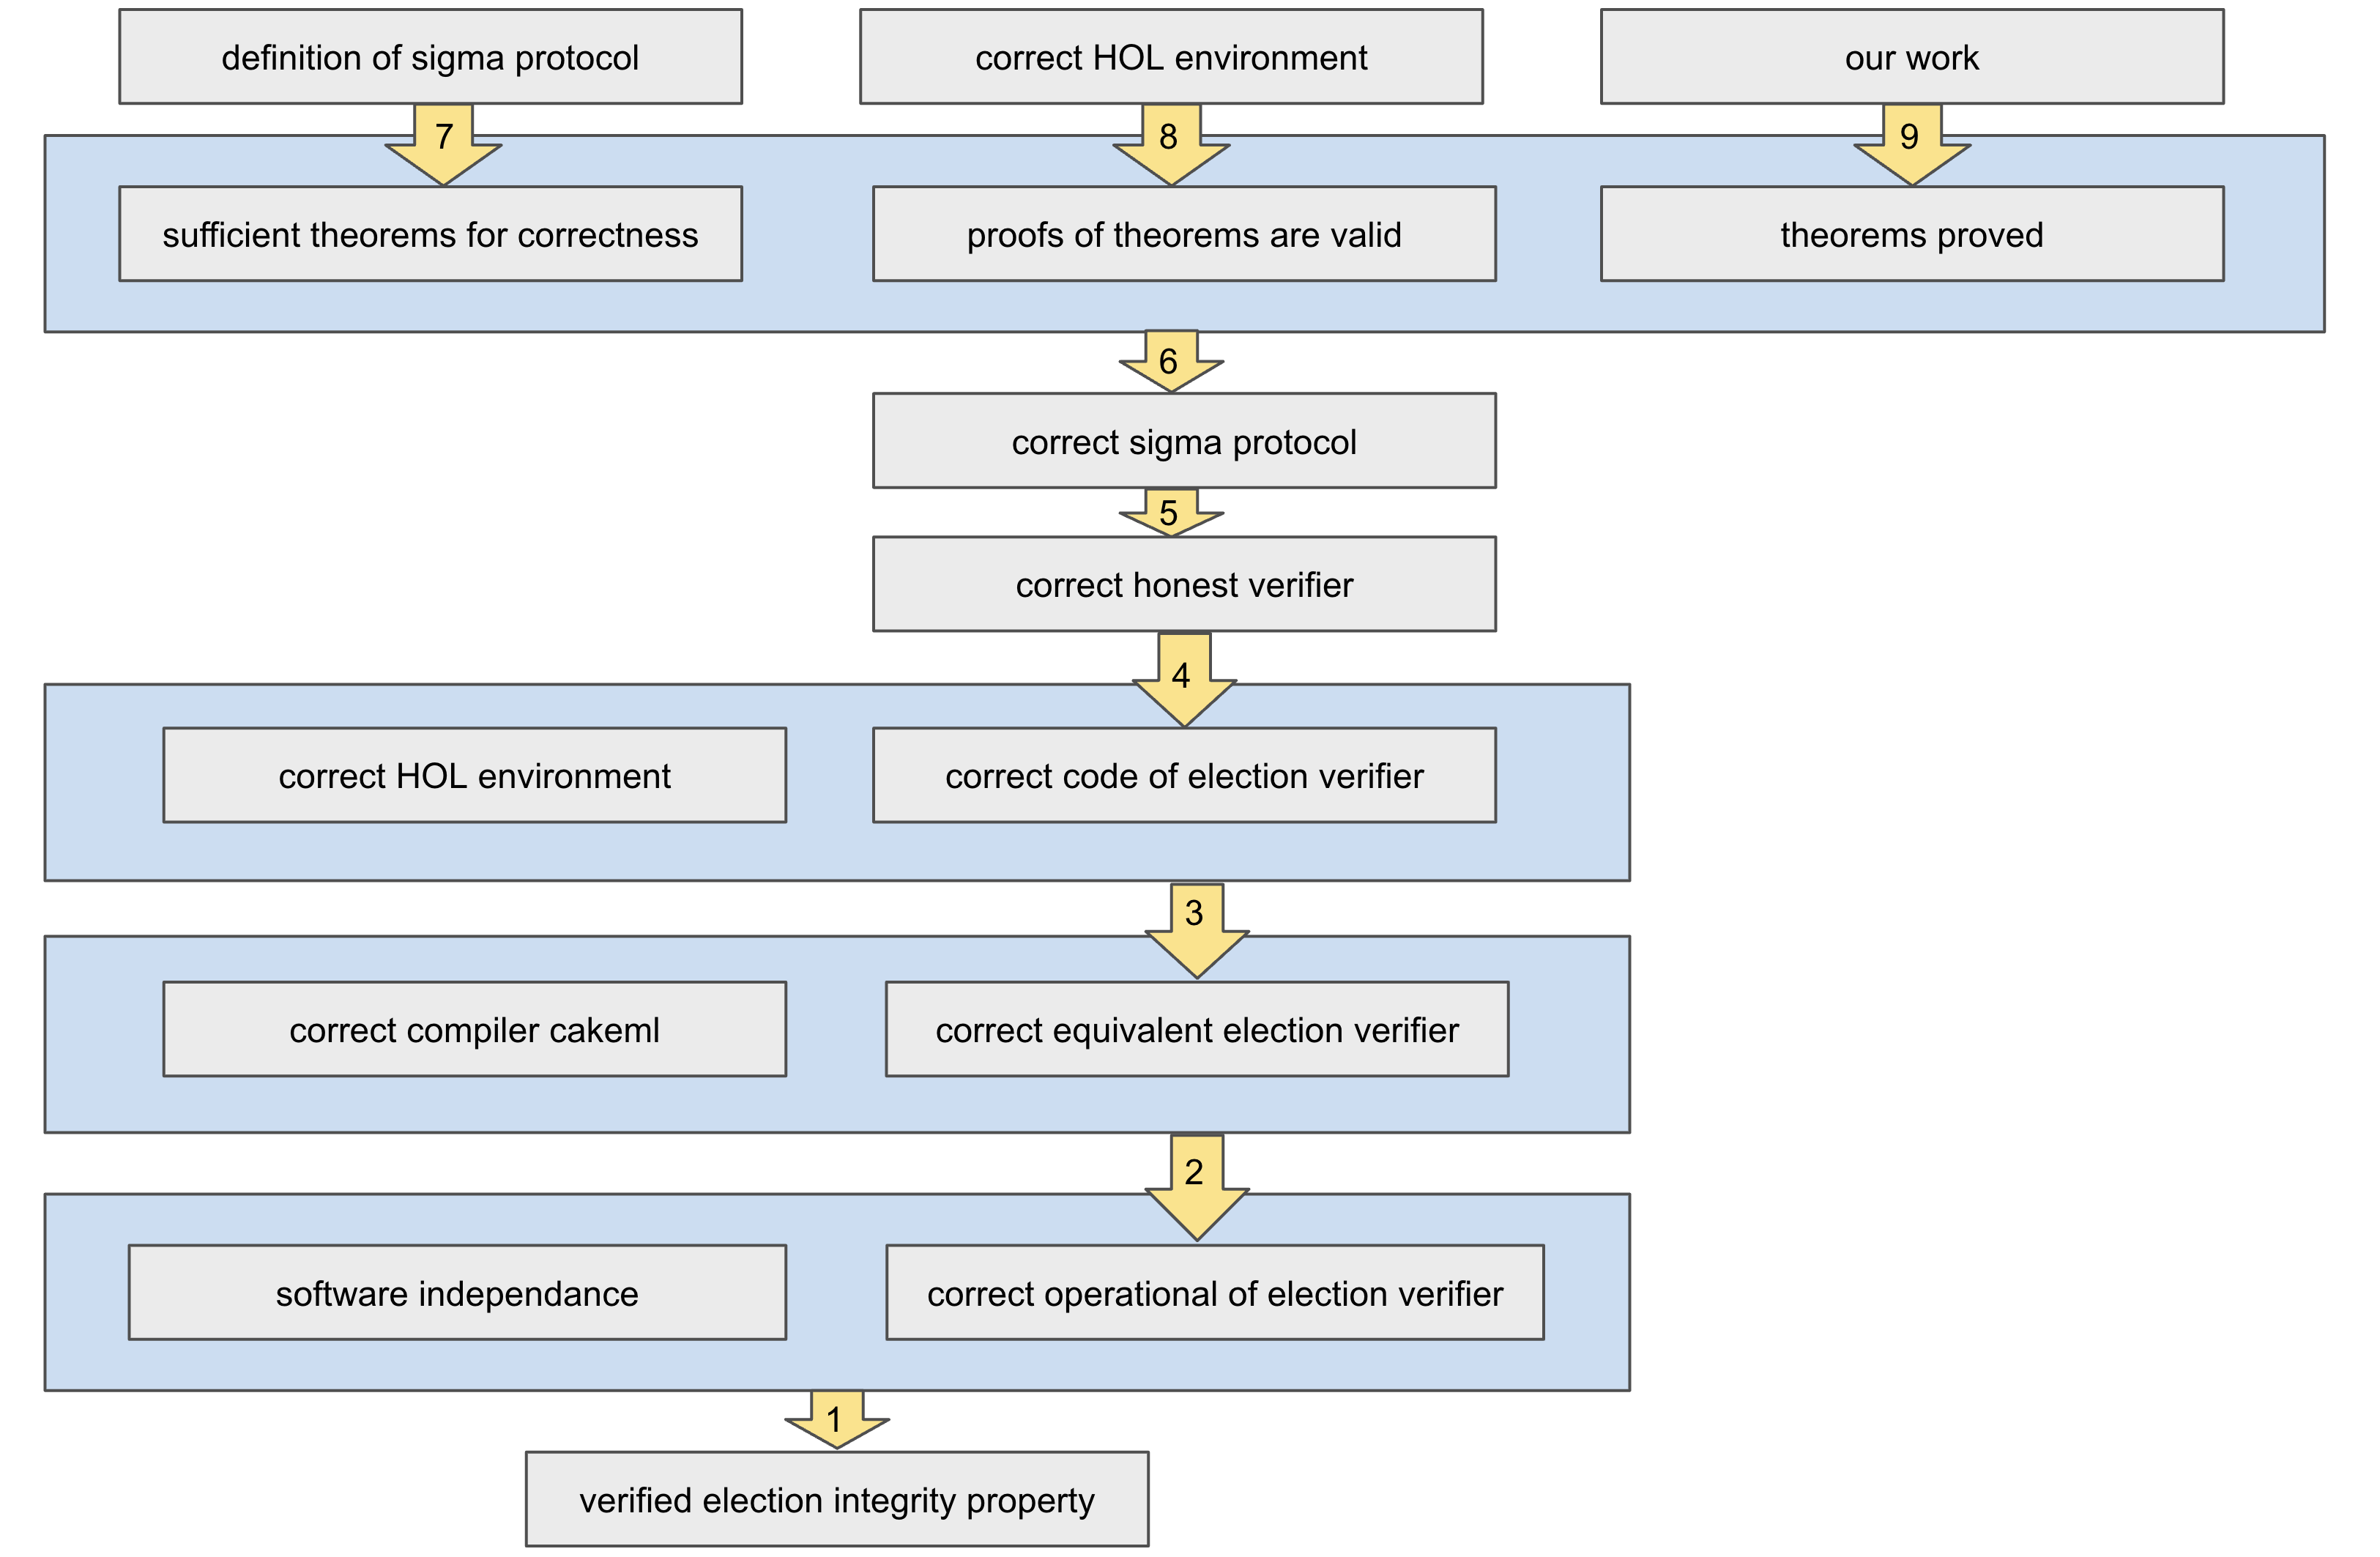
\includegraphics[width=15cm]{figures/proof_graph.png}
  \caption{Logical flow that demonstrates how the guarantee of election integrity is obtained}
\end{figure}%


    The figure demonstrates logical steps that lead to election integrity property being verified. At the bottom is the final goal, at the top is what we have to start, arrows show the implication. We trace from the goal backward and explain how every step is justified:
\begin{enumerate}
    \item Election integrity property holds because the correct election verifier accepts the transcript, supported by the ``Software Independence" concept \cite{Rivest2008OnTN}.
  \item The operational verifier program behaves correctly because the implementation of the equivalent election verifier is correct and it is compiled with verified compiler CakeML.
  \item Implementation of equivalent election verifier is correct because we prove that it is equivalent to original verifier. This proof is valid because HOL4 is verified. 
  \item The implementation of original election verifier is correct because it is calling Honest Verifier.
  \item Honest Verifier is correct because it is contained within proven correct Sigma Protocol.
  \item The Sigma Protocol is correct because
  \begin{enumerate}
      \item We proved theorems
      \item Proofs are valid
      \item Theorems are sufficient
  \end{enumerate}
  \item Theorems are sufficient because of the definition of sigma protocol \cite{damgaard2010sigma}.
  \item Proofs are valid because HOL has been proven to be able to accept only correct proofs.
  \item We proved theorems by developing the code of the proofs.
\end{enumerate}


Therefore, we have demonstrated that the verifier we constructed guarantees election correctness when compiled with the CakeML compiler. Let us now examine the important steps from the above argument in more detail.

\subsection{Sigma protocol correctness}
The correctness of the election verifier is dependent upon the correctness of the Sigma Protocol to which it belongs. In this section, we will explain how the correctness of the composed Sigma Protocol is achieved.

The correctness of the composed Sigma Protocol is dependent on the correctness of its elementary components. We utilized the Schnorr protocol and Protocol Combiners to construct the required Sigma Protocols. The correctness of the composite Sigma Protocol is a consequence of two main proven properties:
\begin{enumerate}
    \item Schnorr Sigma Protocol is correct,
    \item Correctness of the Sigma Protocol is invariant under combinations.
\end{enumerate}
In other words, we demonstrated that if the correct Sigma Protocols are combined by any of our combiners, then the resulting Sigma Protocol is also correct. Therefore, the Schnorr Protocol combined by the Equality (or any other) combiner is correct. Additionally, the Disjoint combination of the Equality Combination of the Schnorr protocol also preserves correctness.

The proofs are valid because the HOL environment guarantees that false proofs cannot be accepted. 
Moreover, the correctness property is given by the thorems which are the definition of the Sigma Protocol, so they suffice for Sigma Protocol Correctness. 
to. We believe that this strategy is sound and that it will allow us to prove the correctness of the election verifier.

We will now provide further details on how we prove the correctness of the Sigma Protocol using its definition. In order to correctly formulate our theorems, we need to clarify certain details. Since Helios uses a Zero Knowledge Proof of Knowledge, we need our Sigma Protocol to satisfy the Zero Knowledge Proof of Knowledge Definition \cite{damgaard2010sigma} discussed in the Background chapter. Namely, the three properties of Completeness, Soundness, and Zero-Knowledge must be satisfied.

\begin{itemize}
\item \textbf{Completeness:} This property can be directly defined by translating English language to mathematics or adopted from Haines et. al. \cite{Haines2019VerifiedVF}. This property states that if the Prover's statement is true, the Verifier always accepts.

\item \textbf{Soundness:} This property is defined probabilistically, which can be challenging to prove using a Proof Assistant. Thankfully, it was shown by Damgard et al. \cite{damgaard2010sigma}, that there is a stronger property Special Soundness, that does not involve probability and implies Soundness. Haines et al. \cite{Haines2021DidYM} adopted the definition of Special Soundness precisely from Damgard et al. \cite{damgaard2010sigma} and formulated in Coq theorem prover, and we will adopt it from Haines. Thus, by proving Special Soundness with this definition, we achieve Soundness. Specifically, this property states:

``For any statement $x$ and any pair of accepting conversations on $x$, $(a,e,z)$, $(a,e',z')$ where $e \neq e'$, one can efficiently compute $w$ such that $(x, w) \in R$"\cite{Haines2021DidYM}.

\item \textbf{Honest-verifier Zero-knowledge:} Honest-Verifier Zero-Knowledge is also defined using probability by Damgard \cite{damgaard2010sigma} as follows 

    ``There exists a polynomial-time simulator M, which on input x and a random e outputs an accepting conversation of the form (a, e, z), with the same probability distribution as conversations between the honest P, V on input x" 
    
    Haines in \cite{Haines2021DidYM} updated the formulation of this property, arguing that it ``suffices to show a bijection between the set of randomness and set of responses such that the output of the respective functions are equal".  We adopt the definition of Honest-verifier zero-knowledge from \cite{Haines2021DidYM} precisely.
\end{itemize}
    By proving the above three theorems we can verify that Sigma protocol is correct by definition.

\section{Summary}
We have developed an election verifier that is proven correct and able to be compiled to verify election integrity. We used Honest Verifier from Sigma Protocol, which is equivalent to the Sigma Protocol of the Election under consideration. To achieve this, we constructed a Sigma Protocol whose Honest Verifier's type signature matched the transcript that needed to be verified. We used elementary components to construct this matching Sigma Protocol.

To prove the correctness of our election verifier, we demonstrated that the Sigma Protocol that contains an equivalent verifier satisfies its definition. This proof relies on the correctness of the components and the invariance of correctness properties under the combinations of Sigma Protocols. We reused the definitions of components and formulations of theorems from \cite{Haines2019VerifiedVF, Haines2021DidYM}.

Our entire development process took place in HOL environment, ensuring that the proofs of our theorems are valid. Additionally, we developed an implementation of the verifier that can be compiled with the CakeML compiler, preserving correctness and producing a proven correct operational election verifier.




                           % related work
\chapter{Implementation}
%%%%%%%%%%%%%%%%%%%%%%%%%%%%%%%%%%%%%%%%%%%%%%%%%%%%%%%%%%%%%%%%%%%%%%%%%%%%%%%%%%%%%%%%%%%%%%%%%%%%%%%%%%%%%%%%%%%%%%%%%%%%%%%%%%%%%%%%%%%%%%%%%%%%%%%%%%%%%%%%%%%%%%%%%%%%%%%%%%%%%%%%
\section{Overview}
%%%%%%%%%%%%%%%%%%%%%%%%%%%%%%%%%%%%%%%%%%%%%%%%%%%%%%%%%%%%%%%%%%%%%%%%%%%%%%%%%%%%%%%%%%%%%%%%%%%%%%%%%%%%%%%%%%%%%%%%%%%%%%%%%%%%%%%%%%%%%%%%%%%%%%%%%%%%%%%%%%%%%%%%%%%%%%%%%%%%%%%%
This chapter provides technical details on the development process, which was previously described at a 
higher level in the Methodology Chapter. Here, we provide definitions of the data types and theorems we 
used, as well as motivation for particular formulations. We do not include proofs, as they are lengthy 
and deserve a separate document. The full proofs and code can be found on 
Git\footnote{https://github.com/Ra6666/crypto_cake}.

We present the definitions of elementary components that we used, definitions 
of the composed Sigma Protocols, and formulations of the theorems to ensure their correctness. 
Additionally, we provide definitions for the data types we utilise and the Verifiers for the election 
transcript.

Recall that our goal is to compose a Sigma Protocol, such that the type signature of its HonestVerifier matches 
the Transcript of our election of interest, the IACR2022 director election. In order to do so, we define the 
following elementary components, which are used as building blocks:
\begin{itemize}
    \item Abstract Sigma Protocol
    \item Disjunctive Combiner
    \item Conjunctive Combiner
    \item Equivalence Combiner
    \item Schnorr Sigma Protocol
\end{itemize}
To verify the IACR2022 director election, we need to verify three types of transcripts: Encryption, Collection, 
and Tallying. To accomplish this, we will compose three Sigma Protocols, each of which matches one of the three 
transcript types. In the following sections, we provide definitions of these composed Sigma Protocols and their 
elementary components.
\begin{itemize}
    \item Schnorr Sigma Protocol
    \item Equivalence Combination of Schnorr Sigma Protocol
    \item Disjunctive Combination of Equivalence Combination of Schnorr Sigma Protocol
\end{itemize}
We will present the formulation of the theorems corresponding to each Sigma Protocol that we utilize:
\begin{itemize}
    \item Completeness
    \item Special Soundness
    \item Honest Verifier Zero-Knowledge
    \item Simulator Correctness
\end{itemize}
We provide definitions for the data types we utilize and the Verifiers for the election transcript:
\begin{itemize}
    \item Result Verifier
    \item Collection Verifier
    \item Enctypion Verifier
\end{itemize}

The mathematical notation in this document may appear unfamiliar at 
first glance, as it reflects the representation of mathematical entities in the HOL logic system, which may 
differ from what we are accustomed to. For example, a Set is a function that takes an element and returns 
either true or false depending on whether it is a member of the set.
\newpage
%%%%%%%%%%%%%%%%%%%%%%%%%%%%%%%%%%%%%%%%%%%%%%%%%%%%%%%%%%%%%%%%%%%%%%%%%%%%%%%%%%%%%%%%%%%%%%%%%%%%%%%%%%%%%%%%%%%%%%%%%%%%%%%%%%%%%%%%%%%%%%%%%%%%%%%%%%%%%%%%%%%%%%%%%%%%%%%%%%%%%%%%
\section{Abstract Components}
%%%%%%%%%%%%%%%%%%%%%%%%%%%%%%%%%%%%%%%%%%%%%%%%%%%%%%%%%%%%%%%%%%%%%%%%%%%%%%%%%%%%%%%%%%%%%%%%%%%%%%%%%%%%%%%%%%%%%%%%%%%%%%%%%%%%%%%%%%%%%%%%%%%%%%%%%%%%%%%%%%%%%%%%%%%%%%%%%%%%%%%%
%------------------------------------------------------------------------------------------------------------------------------------------------------------------------------
\subsubsection{Sigma Protocol Definition}
%------------------------------------------------------------------------------------------------------------------------------------------------------------------------------
We use the following definition for abstract Sigma Protocol. 
\begin{holmath}
    (\ensuremath{\gamma},\,\ensuremath{\epsilon},\,\ensuremath{\varsigma},\,\ensuremath{\sigma},\,\ensuremath{\tau},\,\ensuremath{\chi})\,\HOLTyOp{SigmaProtocol} = \HOLTokenLeftrec{}\\
\,\,\,\HOLFieldName{Statements}\,:\,\ensuremath{\sigma}\,->\,\HOLTyOp{bool};\\
\,\,\,\HOLFieldName{Witnesses}\,:\,\ensuremath{\chi}\,->\,\HOLTyOp{bool};\\
\,\,\,\HOLFieldName{Relation}\,:\,\ensuremath{\sigma}\,->\,\ensuremath{\chi}\,->\,\HOLTyOp{bool};\\
\,\,\,\HOLFieldName{RandomCoins}\,:\,\ensuremath{\varsigma}\,->\,\HOLTyOp{bool};\\
\,\,\,\HOLFieldName{Commitments}\,:\,\ensuremath{\gamma}\,->\,\HOLTyOp{bool};\\
\,\,\,\HOLFieldName{Challenges}\,:\,\ensuremath{\epsilon}\,\HOLTyOp{monoid};\\
\,\,\,\HOLFieldName{Disjoint}\,:\,\ensuremath{\epsilon}\,->\,\ensuremath{\epsilon}\,->\,\HOLTyOp{bool};\\
\,\,\,\HOLFieldName{Responses}\,:\,\ensuremath{\tau}\,->\,\HOLTyOp{bool};\\
\,\,\,\HOLFieldName{Prover_0}\,:\,\ensuremath{\sigma}\,->\,\ensuremath{\chi}\,->\,\ensuremath{\varsigma}\,->\,\ensuremath{\gamma};\\
\,\,\,\HOLFieldName{Prover_1}\,:\,\ensuremath{\sigma}\,->\,\ensuremath{\chi}\,->\,\ensuremath{\varsigma}\,->\,\ensuremath{\gamma}\,->\,\ensuremath{\epsilon}\,->\,\ensuremath{\tau};\\
\,\,\,\HOLFieldName{HonestVerifier}\,:\,\ensuremath{\sigma}\,\HOLTokenProd{}\,\ensuremath{\gamma}\,\HOLTokenProd{}\,\ensuremath{\epsilon}\,\HOLTokenProd{}\,\ensuremath{\tau}\,->\,\HOLTyOp{bool};\\
\,\,\,\HOLFieldName{Extractor}\,:\,\ensuremath{\tau}\,->\,\ensuremath{\tau}\,->\,\ensuremath{\epsilon}\,->\,\ensuremath{\epsilon}\,->\,\ensuremath{\chi};\\
\,\,\,\HOLFieldName{Simulator}\,:\,\ensuremath{\sigma}\,->\,\ensuremath{\tau}\,->\,\ensuremath{\epsilon}\,->\,\ensuremath{\sigma}\,\HOLTokenProd{}\,\ensuremath{\gamma}\,\HOLTokenProd{}\,\ensuremath{\epsilon}\,\HOLTokenProd{}\,\ensuremath{\tau};\\
\,\,\,\HOLFieldName{SimulatorMap}\,:\,\ensuremath{\sigma}\,->\,\ensuremath{\chi}\,->\,\ensuremath{\epsilon}\,->\,\ensuremath{\varsigma}\,->\,\ensuremath{\tau};\\
\,\,\,\HOLFieldName{SimulatorMapInverse}\,:\,\ensuremath{\sigma}\,->\,\ensuremath{\chi}\,->\,\ensuremath{\epsilon}\,->\,\ensuremath{\tau}\,->\,\ensuremath{\varsigma}\\
\HOLTokenRightrec{} 
\end{holmath} 
% It is important to note that in HOL type system, set is a function that takes an element and returns either true 
% if it is a member of the set or false if it is not. Hence, $F: \sigma -> \bool$ denotes a set $F$ of elements of type $\sigma$
This definition captures the functionality required for operation as well as auxiliary functionality to be able to show correctness. 
The type signatures of the components are designed to match each other in the flow of interaction; for example, HonestVerifier input matches the output of Prover\_0 and Simulator.
The protocol allows a Prover to demonstrate to Verifier a possession of the secret witness, such that it is in Relation to a public statement. 
We show how our definition of the protocol relates to its operation:
\begin{enumerate}
\item The Prover picks a random coin and computes a commitment using its function Prover\_0. The Prover sends this commitment to the Verifier.
\item The Verifier picks a challenge and sends it to the Prover.
\item The Prover computes a response using its function Prover\_1 and sends it back to the Verifier, along with the rest of the Transcript.
\item The Verifier checks the Transcript using HonestVerifier. If the Transcript is valid, the Verifier accepts the proof.
\end{enumerate}
To ensure the properties of the Sigma Protocol and for the combiners functionalities, the following functions are required:
\begin{itemize}
\item Extractor: It takes two transcripts and outputs the witness. Required for the proof of Special Soundness property.
\item Simulator: It takes a public transcript and produces a valid commitment for this Transcript without knowing a witness.
\item SimulatorMap and SimulatorMapInverse: These functions are required to prove the Zero-Knowledge property via establishing a 
bijection between Responses and RandomCoins, as described in the Related Work chapter and in \cite{Haines2019VerifiedVF}.
\item Disjoint: The Extractor requires this property to ensure that two challenges are different.
\end{itemize}
A set of Challenges is required to be a Group to ensure that the Extractor can efficiently compute witness given two challenges and, 
therefore, satisfy Special Soundness Property. Note that cross product of Groups also forms a Group; this fact makes a tuple of 
challenges satisfy the abstract definition of Sigma Protocol. \\
%------------------------------------------------------------------------------------------------------------------------------------------------------------------------------
\subsubsection{Disjunctive Sigma Protocol Combiner}
%------------------------------------------------------------------------------------------------------------------------------------------------------------------------------
We use the following definition for the Disjunctive of Sigma Protocols.\\
\\
\HOLConst{SP_or}\,(\HOLFreeVar{sp} :(\ensuremath{\alpha},\,\ensuremath{\beta},\,\ensuremath{\gamma},\,\ensuremath{\epsilon},\,\ensuremath{\delta},\,\ensuremath{\zeta})\,\HOLTyOp{SigmaProtocol})\,\HOLSymConst{=}\\
\HOLTokenLeftrec{}\HOLFieldName{Statements}\,:=\,\HOLFreeVar{sp}.\HOLFieldName{Statements}\,\HOLSymConst{\ensuremath{\times}}\,\HOLFreeVar{sp}.\HOLFieldName{Statements};\,\HOLFieldName{Witnesses}\,:=\,\HOLFreeVar{sp}.\HOLFieldName{Witnesses};\\
\,\,\HOLFieldName{Relation}\,:=\,(\HOLTokenLambda{}((\ensuremath{\HOLBoundVar{s}\sb{\mathrm{1}}} :\ensuremath{\epsilon})\HOLSymConst{,}(\ensuremath{\HOLBoundVar{s}\sb{\mathrm{2}}} :\ensuremath{\epsilon}))\,(\HOLBoundVar{w} :\ensuremath{\zeta}).\,\HOLFreeVar{sp}.\HOLFieldName{Relation}\,\ensuremath{\HOLBoundVar{s}\sb{\mathrm{1}}}\,\HOLBoundVar{w}\,\HOLSymConst{\HOLTokenDisj{}}\,\HOLFreeVar{sp}.\HOLFieldName{Relation}\,\ensuremath{\HOLBoundVar{s}\sb{\mathrm{2}}}\,\HOLBoundVar{w});\\
\,\,\HOLFieldName{RandomCoins}\,:=\,(\HOLFreeVar{sp}.\HOLFieldName{RandomCoins}\,\HOLSymConst{\ensuremath{\times}}\,\HOLFreeVar{sp}.\HOLFieldName{Responses})\,\HOLSymConst{\ensuremath{\times}}\,\HOLFreeVar{sp}.\HOLFieldName{Challenges}.\HOLFieldName{carrier};\\
\,\,\HOLFieldName{Commitments}\,:=\,\HOLFreeVar{sp}.\HOLFieldName{Commitments}\,\HOLSymConst{\ensuremath{\times}}\,\HOLFreeVar{sp}.\HOLFieldName{Commitments};\,\HOLFieldName{Challenges}\,:=\,\HOLFreeVar{sp}.\HOLFieldName{Challenges};\\
\,\,\HOLFieldName{Disjoint}\,:=\,(\HOLTokenLambda{}(\ensuremath{\HOLBoundVar{e}\sb{\mathrm{1}}} :\ensuremath{\beta})\,(\ensuremath{\HOLBoundVar{e}\sb{\mathrm{2}}} :\ensuremath{\beta}).\,\ensuremath{\HOLBoundVar{e}\sb{\mathrm{1}}}\,\HOLSymConst{\HOLTokenNotEqual{}}\,\ensuremath{\HOLBoundVar{e}\sb{\mathrm{2}}});\\
\,\,\HOLFieldName{Responses}\,:=\,(\HOLFreeVar{sp}.\HOLFieldName{Responses}\,\HOLSymConst{\ensuremath{\times}}\,\HOLFreeVar{sp}.\HOLFieldName{Challenges}.\HOLFieldName{carrier})\,\HOLSymConst{\ensuremath{\times}}\,\HOLFreeVar{sp}.\HOLFieldName{Responses};\\
\,\,\HOLFieldName{Prover_0}\,:=\\
\,\,\,\,(\HOLTokenLambda{}((\ensuremath{\HOLBoundVar{s}\sb{\mathrm{1}}} :\ensuremath{\epsilon})\HOLSymConst{,}(\ensuremath{\HOLBoundVar{s}\sb{\mathrm{2}}} :\ensuremath{\epsilon}))\,(\HOLBoundVar{w} :\ensuremath{\zeta})\,(((\HOLBoundVar{r} :\ensuremath{\gamma})\HOLSymConst{,}(\HOLBoundVar{t} :\ensuremath{\delta}))\HOLSymConst{,}(\HOLBoundVar{e} :\ensuremath{\beta})).\\
\,\,\,\,\,\,\,\,\,\HOLKeyword{if}\,\HOLFreeVar{sp}.\HOLFieldName{Relation}\,\ensuremath{\HOLBoundVar{s}\sb{\mathrm{1}}}\,\HOLBoundVar{w}\,\HOLKeyword{then}\\
\,\,\,\,\,\,\,\,\,\,\,(\HOLKeyword{let}\\
\,\,\,\,\,\,\,\,\,\,\,\,\,\,(\ensuremath{\HOLBoundVar{c}\sb{\mathrm{1}}} :\ensuremath{\alpha})\,=\,\HOLFreeVar{sp}.\HOLFieldName{Prover_0}\,\ensuremath{\HOLBoundVar{s}\sb{\mathrm{1}}}\,\HOLBoundVar{w}\,\HOLBoundVar{r};\\
\,\,\,\,\,\,\,\,\,\,\,\,\,\,((\ensuremath{\HOLBoundVar{s}\sb{\mathrm{2}}\sp{\prime{}}} :\ensuremath{\epsilon})\HOLSymConst{,}(\ensuremath{\HOLBoundVar{c}\sb{\mathrm{2}}\sp{\prime{}}} :\ensuremath{\alpha})\HOLSymConst{,}(\ensuremath{\HOLBoundVar{e}\sb{\mathrm{2}}\sp{\prime{}}} :\ensuremath{\beta})\HOLSymConst{,}(\ensuremath{\HOLBoundVar{t}\sb{\mathrm{2}}\sp{\prime{}}} :\ensuremath{\delta}))\,=\,\HOLFreeVar{sp}.\HOLFieldName{Simulator}\,\ensuremath{\HOLBoundVar{s}\sb{\mathrm{2}}}\,\HOLBoundVar{t}\,\HOLBoundVar{e}\\
\,\,\,\,\,\,\,\,\,\,\,\,\HOLKeyword{in}\\
\,\,\,\,\,\,\,\,\,\,\,\,\,\,(\ensuremath{\HOLBoundVar{c}\sb{\mathrm{1}}}\HOLSymConst{,}\ensuremath{\HOLBoundVar{c}\sb{\mathrm{2}}\sp{\prime{}}}))\\
\,\,\,\,\,\,\,\,\,\HOLKeyword{else}\\
\,\,\,\,\,\,\,\,\,\,\,(\HOLKeyword{let}\\
\,\,\,\,\,\,\,\,\,\,\,\,\,\,((\ensuremath{\HOLBoundVar{s}\sb{\mathrm{1}}\sp{\prime{}}} :\ensuremath{\epsilon})\HOLSymConst{,}(\ensuremath{\HOLBoundVar{c}\sb{\mathrm{1}}\sp{\prime{}}} :\ensuremath{\alpha})\HOLSymConst{,}(\ensuremath{\HOLBoundVar{e}\sb{\mathrm{1}}\sp{\prime{}}} :\ensuremath{\beta})\HOLSymConst{,}(\ensuremath{\HOLBoundVar{t}\sb{\mathrm{1}}\sp{\prime{}}} :\ensuremath{\delta}))\,=\,\HOLFreeVar{sp}.\HOLFieldName{Simulator}\,\ensuremath{\HOLBoundVar{s}\sb{\mathrm{1}}}\,\HOLBoundVar{t}\,\HOLBoundVar{e};\\
\,\,\,\,\,\,\,\,\,\,\,\,\,\,(\ensuremath{\HOLBoundVar{c}\sb{\mathrm{2}}} :\ensuremath{\alpha})\,=\,\HOLFreeVar{sp}.\HOLFieldName{Prover_0}\,\ensuremath{\HOLBoundVar{s}\sb{\mathrm{2}}}\,\HOLBoundVar{w}\,\HOLBoundVar{r}\\
\,\,\,\,\,\,\,\,\,\,\,\,\HOLKeyword{in}\\
\,\,\,\,\,\,\,\,\,\,\,\,\,\,(\ensuremath{\HOLBoundVar{c}\sb{\mathrm{1}}\sp{\prime{}}}\HOLSymConst{,}\ensuremath{\HOLBoundVar{c}\sb{\mathrm{2}}})));\\
\,\,\HOLFieldName{Prover_1}\,:=\\
\,\,\,\,(\HOLTokenLambda{}((\ensuremath{\HOLBoundVar{s}\sb{\mathrm{1}}} :\ensuremath{\epsilon})\HOLSymConst{,}(\ensuremath{\HOLBoundVar{s}\sb{\mathrm{2}}} :\ensuremath{\epsilon}))\,(\HOLBoundVar{w} :\ensuremath{\zeta})\,(((\HOLBoundVar{r} :\ensuremath{\gamma})\HOLSymConst{,}(\ensuremath{\HOLBoundVar{t}\sb{\mathrm{1}}} :\ensuremath{\delta}))\HOLSymConst{,}(\ensuremath{\HOLBoundVar{e}\sb{\mathrm{2}}} :\ensuremath{\beta}))\,((\ensuremath{\HOLBoundVar{c}\sb{\mathrm{1}}} :\ensuremath{\alpha})\HOLSymConst{,}(\ensuremath{\HOLBoundVar{c}\sb{\mathrm{2}}} :\ensuremath{\alpha}))\,(\ensuremath{\HOLBoundVar{e}\sb{\mathrm{1}}} :\ensuremath{\beta}).\\
\,\,\,\,\,\,\,\,\,(\HOLKeyword{let}\\
\,\,\,\,\,\,\,\,\,\,\,\,(\ensuremath{\HOLBoundVar{e}\sb{\mathrm{3}}} :\ensuremath{\beta})\,=\,\HOLConst{SP_csub}\,\HOLFreeVar{sp}\,\ensuremath{\HOLBoundVar{e}\sb{\mathrm{1}}}\,\ensuremath{\HOLBoundVar{e}\sb{\mathrm{2}}}\\
\,\,\,\,\,\,\,\,\,\,\HOLKeyword{in}\\
\,\,\,\,\,\,\,\,\,\,\,\,\HOLKeyword{if}\,\HOLFreeVar{sp}.\HOLFieldName{Relation}\,\ensuremath{\HOLBoundVar{s}\sb{\mathrm{1}}}\,\HOLBoundVar{w}\,\HOLKeyword{then}\\
\,\,\,\,\,\,\,\,\,\,\,\,\,\,(\HOLKeyword{let}\\
\,\,\,\,\,\,\,\,\,\,\,\,\,\,\,\,\,((\ensuremath{\HOLBoundVar{s}\sb{\mathrm{2}}\sp{\prime{}}} :\ensuremath{\epsilon})\HOLSymConst{,}(\ensuremath{\HOLBoundVar{c}\sb{\mathrm{2}}\sp{\prime{}}} :\ensuremath{\alpha})\HOLSymConst{,}(\ensuremath{\HOLBoundVar{e}\sb{\mathrm{2}}\sp{\prime{}}} :\ensuremath{\beta})\HOLSymConst{,}(\ensuremath{\HOLBoundVar{t}\sb{\mathrm{2}}\sp{\prime{}}} :\ensuremath{\delta}))\,=\,\HOLFreeVar{sp}.\HOLFieldName{Simulator}\,\ensuremath{\HOLBoundVar{s}\sb{\mathrm{2}}}\,\ensuremath{\HOLBoundVar{t}\sb{\mathrm{1}}}\,\ensuremath{\HOLBoundVar{e}\sb{\mathrm{2}}};\\
\,\,\,\,\,\,\,\,\,\,\,\,\,\,\,\,\,(\ensuremath{\HOLBoundVar{t}\sb{\mathrm{2}}} :\ensuremath{\delta})\,=\,\HOLFreeVar{sp}.\HOLFieldName{Prover_1}\,\ensuremath{\HOLBoundVar{s}\sb{\mathrm{1}}}\,\HOLBoundVar{w}\,\HOLBoundVar{r}\,\ensuremath{\HOLBoundVar{c}\sb{\mathrm{1}}}\,\ensuremath{\HOLBoundVar{e}\sb{\mathrm{3}}}\\
\,\,\,\,\,\,\,\,\,\,\,\,\,\,\,\HOLKeyword{in}\\
\,\,\,\,\,\,\,\,\,\,\,\,\,\,\,\,\,((\ensuremath{\HOLBoundVar{t}\sb{\mathrm{2}}}\HOLSymConst{,}\ensuremath{\HOLBoundVar{e}\sb{\mathrm{3}}})\HOLSymConst{,}\ensuremath{\HOLBoundVar{t}\sb{\mathrm{2}}\sp{\prime{}}}))\\
\,\,\,\,\,\,\,\,\,\,\,\,\HOLKeyword{else}\\
\,\,\,\,\,\,\,\,\,\,\,\,\,\,(\HOLKeyword{let}\\
\,\,\,\,\,\,\,\,\,\,\,\,\,\,\,\,\,((\ensuremath{\HOLBoundVar{s}\sb{\mathrm{1}}\sp{\prime{}}} :\ensuremath{\epsilon})\HOLSymConst{,}(\ensuremath{\HOLBoundVar{c}\sb{\mathrm{1}}\sp{\prime{}}} :\ensuremath{\alpha})\HOLSymConst{,}(\ensuremath{\HOLBoundVar{e}\sb{\mathrm{1}}\sp{\prime{}}} :\ensuremath{\beta})\HOLSymConst{,}(\ensuremath{\HOLBoundVar{t}\sb{\mathrm{1}}\sp{\prime{}}} :\ensuremath{\delta}))\,=\,\HOLFreeVar{sp}.\HOLFieldName{Simulator}\,\ensuremath{\HOLBoundVar{s}\sb{\mathrm{1}}}\,\ensuremath{\HOLBoundVar{t}\sb{\mathrm{1}}}\,\ensuremath{\HOLBoundVar{e}\sb{\mathrm{2}}};\\
\,\,\,\,\,\,\,\,\,\,\,\,\,\,\,\,\,(\ensuremath{\HOLBoundVar{t}\sb{\mathrm{2}}} :\ensuremath{\delta})\,=\,\HOLFreeVar{sp}.\HOLFieldName{Prover_1}\,\ensuremath{\HOLBoundVar{s}\sb{\mathrm{2}}}\,\HOLBoundVar{w}\,\HOLBoundVar{r}\,\ensuremath{\HOLBoundVar{c}\sb{\mathrm{2}}}\,\ensuremath{\HOLBoundVar{e}\sb{\mathrm{3}}}\\
\,\,\,\,\,\,\,\,\,\,\,\,\,\,\,\HOLKeyword{in}\\
\,\,\,\,\,\,\,\,\,\,\,\,\,\,\,\,\,((\ensuremath{\HOLBoundVar{t}\sb{\mathrm{1}}\sp{\prime{}}}\HOLSymConst{,}\ensuremath{\HOLBoundVar{e}\sb{\mathrm{2}}})\HOLSymConst{,}\ensuremath{\HOLBoundVar{t}\sb{\mathrm{2}}}))));\\
\,\,\HOLFieldName{HonestVerifier}\,:=\\
\,\,\,\,(\HOLTokenLambda{}(((\ensuremath{\HOLBoundVar{s}\sb{\mathrm{1}}} :\ensuremath{\epsilon})\HOLSymConst{,}(\ensuremath{\HOLBoundVar{s}\sb{\mathrm{2}}} :\ensuremath{\epsilon}))\HOLSymConst{,}((\ensuremath{\HOLBoundVar{c}\sb{\mathrm{1}}} :\ensuremath{\alpha})\HOLSymConst{,}(\ensuremath{\HOLBoundVar{c}\sb{\mathrm{2}}} :\ensuremath{\alpha}))\HOLSymConst{,}(\ensuremath{\HOLBoundVar{e}\sb{\mathrm{1}}} :\ensuremath{\beta})\HOLSymConst{,}((\ensuremath{\HOLBoundVar{t}\sb{\mathrm{1}}} :\ensuremath{\delta})\HOLSymConst{,}(\ensuremath{\HOLBoundVar{e}\sb{\mathrm{2}}} :\ensuremath{\beta}))\HOLSymConst{,}(\ensuremath{\HOLBoundVar{t}\sb{\mathrm{2}}} :\ensuremath{\delta})).\\
\,\,\,\,\,\,\,\,\,(\HOLKeyword{let}\\
\,\,\,\,\,\,\,\,\,\,\,\,(\ensuremath{\HOLBoundVar{e}\sb{\mathrm{3}}} :\ensuremath{\beta})\,=\,\HOLConst{SP_csub}\,\HOLFreeVar{sp}\,\ensuremath{\HOLBoundVar{e}\sb{\mathrm{1}}}\,\ensuremath{\HOLBoundVar{e}\sb{\mathrm{2}}}\\
\,\,\,\,\,\,\,\,\,\,\HOLKeyword{in}\\
\,\,\,\,\,\,\,\,\,\,\,\,\HOLFreeVar{sp}.\HOLFieldName{HonestVerifier}\,(\ensuremath{\HOLBoundVar{s}\sb{\mathrm{1}}}\HOLSymConst{,}\ensuremath{\HOLBoundVar{c}\sb{\mathrm{1}}}\HOLSymConst{,}\ensuremath{\HOLBoundVar{e}\sb{\mathrm{2}}}\HOLSymConst{,}\ensuremath{\HOLBoundVar{t}\sb{\mathrm{1}}})\,\HOLSymConst{\HOLTokenConj{}}\,\HOLFreeVar{sp}.\HOLFieldName{HonestVerifier}\,(\ensuremath{\HOLBoundVar{s}\sb{\mathrm{2}}}\HOLSymConst{,}\ensuremath{\HOLBoundVar{c}\sb{\mathrm{2}}}\HOLSymConst{,}\ensuremath{\HOLBoundVar{e}\sb{\mathrm{3}}}\HOLSymConst{,}\ensuremath{\HOLBoundVar{t}\sb{\mathrm{2}}})));\\
\,\,\HOLFieldName{Extractor}\,:=\\
\,\,\,\,(\HOLTokenLambda{}(((\ensuremath{\HOLBoundVar{t}\sb{\mathrm{1}}} :\ensuremath{\delta})\HOLSymConst{,}(\ensuremath{\HOLBoundVar{e}\sb{\mathrm{1}}} :\ensuremath{\beta}))\HOLSymConst{,}(\ensuremath{\HOLBoundVar{t}\sb{\mathrm{2}}} :\ensuremath{\delta}))\,(((\ensuremath{\HOLBoundVar{t}\sb{\mathrm{3}}} :\ensuremath{\delta})\HOLSymConst{,}(\ensuremath{\HOLBoundVar{e}\sb{\mathrm{3}}} :\ensuremath{\beta}))\HOLSymConst{,}(\ensuremath{\HOLBoundVar{t}\sb{\mathrm{4}}} :\ensuremath{\delta}))\,(\ensuremath{\HOLBoundVar{e}\sb{\mathrm{5}}} :\ensuremath{\beta})\,(\ensuremath{\HOLBoundVar{e}\sb{\mathrm{6}}} :\ensuremath{\beta}).\\
\,\,\,\,\,\,\,\,\,\HOLKeyword{if}\,\ensuremath{\HOLBoundVar{e}\sb{\mathrm{1}}}\,\HOLSymConst{\HOLTokenNotEqual{}}\,\ensuremath{\HOLBoundVar{e}\sb{\mathrm{3}}}\,\HOLKeyword{then}\,\HOLFreeVar{sp}.\HOLFieldName{Extractor}\,\ensuremath{\HOLBoundVar{t}\sb{\mathrm{1}}}\,\ensuremath{\HOLBoundVar{t}\sb{\mathrm{3}}}\,\ensuremath{\HOLBoundVar{e}\sb{\mathrm{1}}}\,\ensuremath{\HOLBoundVar{e}\sb{\mathrm{3}}}\\
\,\,\,\,\,\,\,\,\,\HOLKeyword{else}\\
\,\,\,\,\,\,\,\,\,\,\,(\HOLKeyword{let}\\
\,\,\,\,\,\,\,\,\,\,\,\,\,\,(\ensuremath{\HOLBoundVar{e}\sb{\mathrm{2}}} :\ensuremath{\beta})\,=\,\HOLConst{SP_csub}\,\HOLFreeVar{sp}\,\ensuremath{\HOLBoundVar{e}\sb{\mathrm{5}}}\,\ensuremath{\HOLBoundVar{e}\sb{\mathrm{1}}};\\
\,\,\,\,\,\,\,\,\,\,\,\,\,\,(\ensuremath{\HOLBoundVar{e}\sb{\mathrm{4}}} :\ensuremath{\beta})\,=\,\HOLConst{SP_csub}\,\HOLFreeVar{sp}\,\ensuremath{\HOLBoundVar{e}\sb{\mathrm{6}}}\,\ensuremath{\HOLBoundVar{e}\sb{\mathrm{3}}}\\
\,\,\,\,\,\,\,\,\,\,\,\,\HOLKeyword{in}\\
\,\,\,\,\,\,\,\,\,\,\,\,\,\,\HOLFreeVar{sp}.\HOLFieldName{Extractor}\,\ensuremath{\HOLBoundVar{t}\sb{\mathrm{2}}}\,\ensuremath{\HOLBoundVar{t}\sb{\mathrm{4}}}\,\ensuremath{\HOLBoundVar{e}\sb{\mathrm{2}}}\,\ensuremath{\HOLBoundVar{e}\sb{\mathrm{4}}}));\\
\,\,\HOLFieldName{Simulator}\,:=\\
\,\,\,\,(\HOLTokenLambda{}((\ensuremath{\HOLBoundVar{s}\sb{\mathrm{1}}} :\ensuremath{\epsilon})\HOLSymConst{,}(\ensuremath{\HOLBoundVar{s}\sb{\mathrm{2}}} :\ensuremath{\epsilon}))\,(((\ensuremath{\HOLBoundVar{t}\sb{\mathrm{1}}} :\ensuremath{\delta})\HOLSymConst{,}(\ensuremath{\HOLBoundVar{e}\sb{\mathrm{1}}} :\ensuremath{\beta}))\HOLSymConst{,}(\ensuremath{\HOLBoundVar{t}\sb{\mathrm{2}}} :\ensuremath{\delta}))\,(\ensuremath{\HOLBoundVar{e}\sb{\mathrm{2}}} :\ensuremath{\beta}).\\
\,\,\,\,\,\,\,\,\,(\HOLKeyword{let}\\
\,\,\,\,\,\,\,\,\,\,\,\,((\ensuremath{\HOLBoundVar{s}\sb{\mathrm{1}}\sp{\prime{}}} :\ensuremath{\epsilon})\HOLSymConst{,}(\ensuremath{\HOLBoundVar{c}\sb{\mathrm{1}}\sp{\prime{}}} :\ensuremath{\alpha})\HOLSymConst{,}(\ensuremath{\HOLBoundVar{e}\sb{\mathrm{1}}\sp{\prime{}}} :\ensuremath{\beta})\HOLSymConst{,}(\ensuremath{\HOLBoundVar{t}\sb{\mathrm{1}}\sp{\prime{}}} :\ensuremath{\delta}))\,=\,\HOLFreeVar{sp}.\HOLFieldName{Simulator}\,\ensuremath{\HOLBoundVar{s}\sb{\mathrm{1}}}\,\ensuremath{\HOLBoundVar{t}\sb{\mathrm{1}}}\,\ensuremath{\HOLBoundVar{e}\sb{\mathrm{1}}};\\
\,\,\,\,\,\,\,\,\,\,\,\,(\ensuremath{\HOLBoundVar{e}\sb{\mathrm{3}}} :\ensuremath{\beta})\,=\,\HOLConst{SP_csub}\,\HOLFreeVar{sp}\,\ensuremath{\HOLBoundVar{e}\sb{\mathrm{2}}}\,\ensuremath{\HOLBoundVar{e}\sb{\mathrm{1}}};\\
\,\,\,\,\,\,\,\,\,\,\,\,((\ensuremath{\HOLBoundVar{s}\sb{\mathrm{2}}\sp{\prime{}}} :\ensuremath{\epsilon})\HOLSymConst{,}(\ensuremath{\HOLBoundVar{c}\sb{\mathrm{2}}\sp{\prime{}}} :\ensuremath{\alpha})\HOLSymConst{,}(\ensuremath{\HOLBoundVar{e}\sb{\mathrm{2}}\sp{\prime{}}} :\ensuremath{\beta})\HOLSymConst{,}(\ensuremath{\HOLBoundVar{t}\sb{\mathrm{2}}\sp{\prime{}}} :\ensuremath{\delta}))\,=\,\HOLFreeVar{sp}.\HOLFieldName{Simulator}\,\ensuremath{\HOLBoundVar{s}\sb{\mathrm{2}}}\,\ensuremath{\HOLBoundVar{t}\sb{\mathrm{2}}}\,\ensuremath{\HOLBoundVar{e}\sb{\mathrm{3}}}\\
\,\,\,\,\,\,\,\,\,\,\HOLKeyword{in}\\
\,\,\,\,\,\,\,\,\,\,\,\,((\ensuremath{\HOLBoundVar{s}\sb{\mathrm{1}}}\HOLSymConst{,}\ensuremath{\HOLBoundVar{s}\sb{\mathrm{2}}})\HOLSymConst{,}(\ensuremath{\HOLBoundVar{c}\sb{\mathrm{1}}\sp{\prime{}}}\HOLSymConst{,}\ensuremath{\HOLBoundVar{c}\sb{\mathrm{2}}\sp{\prime{}}})\HOLSymConst{,}\ensuremath{\HOLBoundVar{e}\sb{\mathrm{2}}}\HOLSymConst{,}(\ensuremath{\HOLBoundVar{t}\sb{\mathrm{1}}\sp{\prime{}}}\HOLSymConst{,}\ensuremath{\HOLBoundVar{e}\sb{\mathrm{1}}})\HOLSymConst{,}\ensuremath{\HOLBoundVar{t}\sb{\mathrm{2}}\sp{\prime{}}})));\\
\,\,\HOLFieldName{SimulatorMap}\,:=\\
\,\,\,\,(\HOLTokenLambda{}((\ensuremath{\HOLBoundVar{s}\sb{\mathrm{1}}} :\ensuremath{\epsilon})\HOLSymConst{,}(\ensuremath{\HOLBoundVar{s}\sb{\mathrm{2}}} :\ensuremath{\epsilon}))\,(\HOLBoundVar{w} :\ensuremath{\zeta})\,(\ensuremath{\HOLBoundVar{e}\sb{\mathrm{1}}} :\ensuremath{\beta})\,(((\HOLBoundVar{r} :\ensuremath{\gamma})\HOLSymConst{,}(\HOLBoundVar{t} :\ensuremath{\delta}))\HOLSymConst{,}(\ensuremath{\HOLBoundVar{e}\sb{\mathrm{2}}} :\ensuremath{\beta})).\\
\,\,\,\,\,\,\,\,\,(\HOLKeyword{let}\\
\,\,\,\,\,\,\,\,\,\,\,\,(\ensuremath{\HOLBoundVar{e}\sb{\mathrm{3}}} :\ensuremath{\beta})\,=\,\HOLConst{SP_csub}\,\HOLFreeVar{sp}\,\ensuremath{\HOLBoundVar{e}\sb{\mathrm{1}}}\,\ensuremath{\HOLBoundVar{e}\sb{\mathrm{2}}}\\
\,\,\,\,\,\,\,\,\,\,\HOLKeyword{in}\\
\,\,\,\,\,\,\,\,\,\,\,\,\HOLKeyword{if}\,\HOLFreeVar{sp}.\HOLFieldName{Relation}\,\ensuremath{\HOLBoundVar{s}\sb{\mathrm{1}}}\,\HOLBoundVar{w}\,\HOLKeyword{then}\,(\HOLKeyword{let}\,(\ensuremath{\HOLBoundVar{t}\sb{\mathrm{1}}} :\ensuremath{\delta})\,=\,\HOLFreeVar{sp}.\HOLFieldName{SimulatorMap}\,\ensuremath{\HOLBoundVar{s}\sb{\mathrm{1}}}\,\HOLBoundVar{w}\,\ensuremath{\HOLBoundVar{e}\sb{\mathrm{3}}}\,\HOLBoundVar{r}\,\HOLKeyword{in}\,((\ensuremath{\HOLBoundVar{t}\sb{\mathrm{1}}}\HOLSymConst{,}\ensuremath{\HOLBoundVar{e}\sb{\mathrm{3}}})\HOLSymConst{,}\HOLBoundVar{t}))\\
\,\,\,\,\,\,\,\,\,\,\,\,\HOLKeyword{else}\,(\HOLKeyword{let}\,(\ensuremath{\HOLBoundVar{t}\sb{\mathrm{2}}} :\ensuremath{\delta})\,=\,\HOLFreeVar{sp}.\HOLFieldName{SimulatorMap}\,\ensuremath{\HOLBoundVar{s}\sb{\mathrm{2}}}\,\HOLBoundVar{w}\,\ensuremath{\HOLBoundVar{e}\sb{\mathrm{3}}}\,\HOLBoundVar{r}\,\HOLKeyword{in}\,((\HOLBoundVar{t}\HOLSymConst{,}\ensuremath{\HOLBoundVar{e}\sb{\mathrm{2}}})\HOLSymConst{,}\ensuremath{\HOLBoundVar{t}\sb{\mathrm{2}}}))));\\
\,\,\HOLFieldName{SimulatorMapInverse}\,:=\\
\,\,\,\,(\HOLTokenLambda{}((\ensuremath{\HOLBoundVar{s}\sb{\mathrm{1}}} :\ensuremath{\epsilon})\HOLSymConst{,}(\ensuremath{\HOLBoundVar{s}\sb{\mathrm{2}}} :\ensuremath{\epsilon}))\,(\HOLBoundVar{w} :\ensuremath{\zeta})\,(\ensuremath{\HOLBoundVar{e}\sb{\mathrm{1}}} :\ensuremath{\beta})\,(((\ensuremath{\HOLBoundVar{t}\sb{\mathrm{1}}} :\ensuremath{\delta})\HOLSymConst{,}(\ensuremath{\HOLBoundVar{e}\sb{\mathrm{2}}} :\ensuremath{\beta}))\HOLSymConst{,}(\ensuremath{\HOLBoundVar{t}\sb{\mathrm{2}}} :\ensuremath{\delta})).\\
\,\,\,\,\,\,\,\,\,(\HOLKeyword{let}\\
\,\,\,\,\,\,\,\,\,\,\,\,(\ensuremath{\HOLBoundVar{e}\sb{\mathrm{3}}} :\ensuremath{\beta})\,=\,\HOLConst{SP_csub}\,\HOLFreeVar{sp}\,\ensuremath{\HOLBoundVar{e}\sb{\mathrm{1}}}\,\ensuremath{\HOLBoundVar{e}\sb{\mathrm{2}}}\\
\,\,\,\,\,\,\,\,\,\,\HOLKeyword{in}\\
\,\,\,\,\,\,\,\,\,\,\,\,\HOLKeyword{if}\,\HOLFreeVar{sp}.\HOLFieldName{Relation}\,\ensuremath{\HOLBoundVar{s}\sb{\mathrm{1}}}\,\HOLBoundVar{w}\,\HOLKeyword{then}\\
\,\,\,\,\,\,\,\,\,\,\,\,\,\,(\HOLKeyword{let}\,(\HOLBoundVar{r} :\ensuremath{\gamma})\,=\,\HOLFreeVar{sp}.\HOLFieldName{SimulatorMapInverse}\,\ensuremath{\HOLBoundVar{s}\sb{\mathrm{1}}}\,\HOLBoundVar{w}\,\ensuremath{\HOLBoundVar{e}\sb{\mathrm{2}}}\,\ensuremath{\HOLBoundVar{t}\sb{\mathrm{1}}}\,\HOLKeyword{in}\,((\HOLBoundVar{r}\HOLSymConst{,}\ensuremath{\HOLBoundVar{t}\sb{\mathrm{2}}})\HOLSymConst{,}\ensuremath{\HOLBoundVar{e}\sb{\mathrm{3}}}))\\
\,\,\,\,\,\,\,\,\,\,\,\,\HOLKeyword{else}\,(\HOLKeyword{let}\,(\HOLBoundVar{r} :\ensuremath{\gamma})\,=\,\HOLFreeVar{sp}.\HOLFieldName{SimulatorMapInverse}\,\ensuremath{\HOLBoundVar{s}\sb{\mathrm{2}}}\,\HOLBoundVar{w}\,\ensuremath{\HOLBoundVar{e}\sb{\mathrm{3}}}\,\ensuremath{\HOLBoundVar{t}\sb{\mathrm{2}}}\,\HOLKeyword{in}\,((\HOLBoundVar{r}\HOLSymConst{,}\ensuremath{\HOLBoundVar{t}\sb{\mathrm{1}}})\HOLSymConst{,}\ensuremath{\HOLBoundVar{e}\sb{\mathrm{2}}}))))\HOLTokenRightrec{}
The Disjunctive Combiner allows us to build more complicated Sigma Protocols out of simpler
ones. The statement of Disjunctive Combination consists of two values, at least one of which is in Relation to the witness. 
The Prover wants to demonstrate that they know the witness. The operation is similar to the
abstract Sigma Protocol, and the following shows how our definition relates to the operation.
\begin{enumerate}
\item The Prover picks two random coins and computes a commitment using function Prover\_0. 
Function Prover\_0 returns two values, one is simulated without knowledge of the secret witness, and another is real and computed by 
Prover\_0 function of underlying sigma protocol, using knowledge of the witness. Then Prover sends this commitment to the Verifier.
\item The Verifier picks a challenge and sends it to the Prover. 
\item The Prover computes a response using function Prover\_1; this response contains one real value and one simulated without knowledge of the secret. 
Then The Prover sends it back to the Verifier along with the rest of the Transcript.
\item The Verifier checks the Transcript using HonestVerifier. If the Transcript is valid, the Verifier accepts the proof. The HonestVerifier calls 
HonestVerifier of underlying Sigma Protocol twice, and both calls have to accept. Even though one Transcript is simulated, it must be accepted because 
the Simulator function produces the correct Transcript. 
\end{enumerate}
The Disjoint property in the Disjunctive Combination of Sigma protocols refers to the requirement that the challenge must be distinct for the 
Extractor to compute the secret. This is crucial for the Special Soundness property, which asserts that the secret can be computed if a prover 
can answer two different challenges for the same initial commitment.
Since the challenge is a single value, Disjoint becomes inequality for Disjunctive Combination.

In the context of a disjunctive combination, the Prover is providing a proof for at least one of two statements. The Verifier then challenges the 
Prover, who must respond correctly to maintain the validity of the proof. If the challenges were not distinct (i.e., if they were equal), the 
Prover could respond correctly to one challenge and incorrectly to the other yet still have the overall proof be accepted. This would violate the 
Special Soundness property and allow a dishonest prover to convince a verifier of a false statement.

Extractor of Disjunctive Combination is designed to take two responses, two challenges and compute the witness. 
The function first checks if the challenges belonging to responses are not equal. If they are not equal, it calls the Extractor function of the 
underlying Sigma Protocol because, in the case of unequal challenges, the Extractor can directly compute the witness. Otherwise, if the challenges 
are equal, then it means that the same challenge was used in both transcripts. In this case, the Extractor cannot directly compute the witness. 
Therefore, it computes two new challenges for itself. 

Simulator of Disjunctive Combination computes two commitments and returns an accepting transcript without knowledge of the secret. 

SimulatorMap and SimulatorMapInverse are designed to match each other and be able still to 
provide a bijection using a more complicated transcript.\\
%------------------------------------------------------------------------------------------------------------------------------------------------------------------------------
\subsubsection{Conjunctive Sigma Protocol Combiner}
%------------------------------------------------------------------------------------------------------------------------------------------------------------------------------
We use the following definition for the Conjunctive Combiner of Sigma Protocol. \\
\HOLTokenTurnstile{}\HOLConst{SP_and}\,(\ensuremath{\HOLFreeVar{S}\sb{\mathrm{1}}} :(\ensuremath{\alpha},\,\ensuremath{\gamma},\,\ensuremath{\epsilon},\,\ensuremath{\eta},\,\ensuremath{\iota},\,'k)\,\HOLTyOp{SigmaProtocol})\\
\,\,\,\,\,\,\,\,\,(\ensuremath{\HOLFreeVar{S}\sb{\mathrm{2}}} :(\ensuremath{\beta},\,\ensuremath{\delta},\,\ensuremath{\zeta},\,\ensuremath{\theta},\,\ensuremath{\kappa},\,\ensuremath{\mu})\,\HOLTyOp{SigmaProtocol})\,\HOLSymConst{=}\\
\,\,\,\,\,\,\,\HOLTokenLeftrec{}\HOLFieldName{Statements}\,:=\,\ensuremath{\HOLFreeVar{S}\sb{\mathrm{1}}}.\HOLFieldName{Statements}\,\HOLSymConst{\ensuremath{\times}}\,\ensuremath{\HOLFreeVar{S}\sb{\mathrm{2}}}.\HOLFieldName{Statements};\\
\,\,\,\,\,\,\,\,\,\HOLFieldName{Witnesses}\,:=\,\ensuremath{\HOLFreeVar{S}\sb{\mathrm{1}}}.\HOLFieldName{Witnesses}\,\HOLSymConst{\ensuremath{\times}}\,\ensuremath{\HOLFreeVar{S}\sb{\mathrm{2}}}.\HOLFieldName{Witnesses};\\
\,\,\,\,\,\,\,\,\,\HOLFieldName{Relation}\,:=\\
\,\,\,\,\,\,\,\,\,\,\,(\HOLTokenLambda{}((\ensuremath{\HOLBoundVar{s}\sb{\mathrm{1}}} :\ensuremath{\eta})\HOLSymConst{,}(\ensuremath{\HOLBoundVar{s}\sb{\mathrm{2}}} :\ensuremath{\theta}))\,((\ensuremath{\HOLBoundVar{w}\sb{\mathrm{1}}} :'k)\HOLSymConst{,}(\ensuremath{\HOLBoundVar{w}\sb{\mathrm{2}}} :\ensuremath{\mu})).\\
\,\,\,\,\,\,\,\,\,\,\,\,\,\,\,\,\ensuremath{\HOLFreeVar{S}\sb{\mathrm{1}}}.\HOLFieldName{Relation}\,\ensuremath{\HOLBoundVar{s}\sb{\mathrm{1}}}\,\ensuremath{\HOLBoundVar{w}\sb{\mathrm{1}}}\,\HOLSymConst{\HOLTokenConj{}}\,\ensuremath{\HOLFreeVar{S}\sb{\mathrm{2}}}.\HOLFieldName{Relation}\,\ensuremath{\HOLBoundVar{s}\sb{\mathrm{2}}}\,\ensuremath{\HOLBoundVar{w}\sb{\mathrm{2}}});\\
\,\,\,\,\,\,\,\,\,\HOLFieldName{RandomCoins}\,:=\,\ensuremath{\HOLFreeVar{S}\sb{\mathrm{1}}}.\HOLFieldName{RandomCoins}\,\HOLSymConst{\ensuremath{\times}}\,\ensuremath{\HOLFreeVar{S}\sb{\mathrm{2}}}.\HOLFieldName{RandomCoins};\\
\,\,\,\,\,\,\,\,\,\HOLFieldName{Commitments}\,:=\,\ensuremath{\HOLFreeVar{S}\sb{\mathrm{1}}}.\HOLFieldName{Commitments}\,\HOLSymConst{\ensuremath{\times}}\,\ensuremath{\HOLFreeVar{S}\sb{\mathrm{2}}}.\HOLFieldName{Commitments};\\
\,\,\,\,\,\,\,\,\,\HOLFieldName{Challenges}\,:=\,\HOLConst{Gcross}\,\ensuremath{\HOLFreeVar{S}\sb{\mathrm{1}}}.\HOLFieldName{Challenges}\,\ensuremath{\HOLFreeVar{S}\sb{\mathrm{2}}}.\HOLFieldName{Challenges};\\
\,\,\,\,\,\,\,\,\,\HOLFieldName{Disjoint}\,:=\\
\,\,\,\,\,\,\,\,\,\,\,(\HOLTokenLambda{}((\HOLBoundVar{a} :\ensuremath{\gamma})\HOLSymConst{,}(\HOLBoundVar{b} :\ensuremath{\delta}))\,((\HOLBoundVar{c} :\ensuremath{\gamma})\HOLSymConst{,}(\HOLBoundVar{d} :\ensuremath{\delta})).\\
\,\,\,\,\,\,\,\,\,\,\,\,\,\,\,\,\ensuremath{\HOLFreeVar{S}\sb{\mathrm{1}}}.\HOLFieldName{Disjoint}\,\HOLBoundVar{a}\,\HOLBoundVar{c}\,\HOLSymConst{\HOLTokenConj{}}\,\ensuremath{\HOLFreeVar{S}\sb{\mathrm{2}}}.\HOLFieldName{Disjoint}\,\HOLBoundVar{b}\,\HOLBoundVar{d});\\
\,\,\,\,\,\,\,\,\,\HOLFieldName{Responses}\,:=\,\ensuremath{\HOLFreeVar{S}\sb{\mathrm{1}}}.\HOLFieldName{Responses}\,\HOLSymConst{\ensuremath{\times}}\,\ensuremath{\HOLFreeVar{S}\sb{\mathrm{2}}}.\HOLFieldName{Responses};\\
\,\,\,\,\,\,\,\,\,\HOLFieldName{Prover_0}\,:=\\
\,\,\,\,\,\,\,\,\,\,\,(\HOLTokenLambda{}((\ensuremath{\HOLBoundVar{s}\sb{\mathrm{1}}} :\ensuremath{\eta})\HOLSymConst{,}(\ensuremath{\HOLBoundVar{s}\sb{\mathrm{2}}} :\ensuremath{\theta}))\,((\ensuremath{\HOLBoundVar{w}\sb{\mathrm{1}}} :'k)\HOLSymConst{,}(\ensuremath{\HOLBoundVar{w}\sb{\mathrm{2}}} :\ensuremath{\mu}))\\
\,\,\,\,\,\,\,\,\,\,\,\,\,\,\,\,((\ensuremath{\HOLBoundVar{r}\sb{\mathrm{1}}} :\ensuremath{\epsilon})\HOLSymConst{,}(\ensuremath{\HOLBoundVar{r}\sb{\mathrm{2}}} :\ensuremath{\zeta})).\\
\,\,\,\,\,\,\,\,\,\,\,\,\,\,\,\,(\ensuremath{\HOLFreeVar{S}\sb{\mathrm{1}}}.\HOLFieldName{Prover_0}\,\ensuremath{\HOLBoundVar{s}\sb{\mathrm{1}}}\,\ensuremath{\HOLBoundVar{w}\sb{\mathrm{1}}}\,\ensuremath{\HOLBoundVar{r}\sb{\mathrm{1}}}\HOLSymConst{,}\ensuremath{\HOLFreeVar{S}\sb{\mathrm{2}}}.\HOLFieldName{Prover_0}\,\ensuremath{\HOLBoundVar{s}\sb{\mathrm{2}}}\,\ensuremath{\HOLBoundVar{w}\sb{\mathrm{2}}}\,\ensuremath{\HOLBoundVar{r}\sb{\mathrm{2}}}));\\
\,\,\,\,\,\,\,\,\,\HOLFieldName{Prover_1}\,:=\\
\,\,\,\,\,\,\,\,\,\,\,(\HOLTokenLambda{}((\ensuremath{\HOLBoundVar{s}\sb{\mathrm{1}}} :\ensuremath{\eta})\HOLSymConst{,}(\ensuremath{\HOLBoundVar{s}\sb{\mathrm{2}}} :\ensuremath{\theta}))\,((\ensuremath{\HOLBoundVar{w}\sb{\mathrm{1}}} :'k)\HOLSymConst{,}(\ensuremath{\HOLBoundVar{w}\sb{\mathrm{2}}} :\ensuremath{\mu}))\\
\,\,\,\,\,\,\,\,\,\,\,\,\,\,\,\,((\ensuremath{\HOLBoundVar{r}\sb{\mathrm{1}}} :\ensuremath{\epsilon})\HOLSymConst{,}(\ensuremath{\HOLBoundVar{r}\sb{\mathrm{2}}} :\ensuremath{\zeta}))\,((\ensuremath{\HOLBoundVar{c}\sb{\mathrm{1}}} :\ensuremath{\alpha})\HOLSymConst{,}(\ensuremath{\HOLBoundVar{c}\sb{\mathrm{2}}} :\ensuremath{\beta}))\\
\,\,\,\,\,\,\,\,\,\,\,\,\,\,\,\,((\ensuremath{\HOLBoundVar{e}\sb{\mathrm{1}}} :\ensuremath{\gamma})\HOLSymConst{,}(\ensuremath{\HOLBoundVar{e}\sb{\mathrm{2}}} :\ensuremath{\delta})).\\
\,\,\,\,\,\,\,\,\,\,\,\,\,\,\,\,(\ensuremath{\HOLFreeVar{S}\sb{\mathrm{1}}}.\HOLFieldName{Prover_1}\,\ensuremath{\HOLBoundVar{s}\sb{\mathrm{1}}}\,\ensuremath{\HOLBoundVar{w}\sb{\mathrm{1}}}\,\ensuremath{\HOLBoundVar{r}\sb{\mathrm{1}}}\,\ensuremath{\HOLBoundVar{c}\sb{\mathrm{1}}}\,\ensuremath{\HOLBoundVar{e}\sb{\mathrm{1}}}\HOLSymConst{,}\ensuremath{\HOLFreeVar{S}\sb{\mathrm{2}}}.\HOLFieldName{Prover_1}\,\ensuremath{\HOLBoundVar{s}\sb{\mathrm{2}}}\,\ensuremath{\HOLBoundVar{w}\sb{\mathrm{2}}}\,\ensuremath{\HOLBoundVar{r}\sb{\mathrm{2}}}\,\ensuremath{\HOLBoundVar{c}\sb{\mathrm{2}}}\,\ensuremath{\HOLBoundVar{e}\sb{\mathrm{2}}}));\\
\,\,\,\,\,\,\,\,\,\HOLFieldName{HonestVerifier}\,:=\\
\,\,\,\,\,\,\,\,\,\,\,(\HOLTokenLambda{}(((\ensuremath{\HOLBoundVar{s}\sb{\mathrm{1}}} :\ensuremath{\eta})\HOLSymConst{,}(\ensuremath{\HOLBoundVar{s}\sb{\mathrm{2}}} :\ensuremath{\theta}))\HOLSymConst{,}((\ensuremath{\HOLBoundVar{c}\sb{\mathrm{1}}} :\ensuremath{\alpha})\HOLSymConst{,}(\ensuremath{\HOLBoundVar{c}\sb{\mathrm{2}}} :\ensuremath{\beta}))\HOLSymConst{,}\\
\,\,\,\,\,\,\,\,\,\,\,\,\,\,\,\,\,((\ensuremath{\HOLBoundVar{e}\sb{\mathrm{1}}} :\ensuremath{\gamma})\HOLSymConst{,}(\ensuremath{\HOLBoundVar{e}\sb{\mathrm{2}}} :\ensuremath{\delta}))\HOLSymConst{,}(\ensuremath{\HOLBoundVar{t}\sb{\mathrm{1}}} :\ensuremath{\iota})\HOLSymConst{,}(\ensuremath{\HOLBoundVar{t}\sb{\mathrm{2}}} :\ensuremath{\kappa})).\\
\,\,\,\,\,\,\,\,\,\,\,\,\,\,\,\,\ensuremath{\HOLFreeVar{S}\sb{\mathrm{1}}}.\HOLFieldName{HonestVerifier}\,(\ensuremath{\HOLBoundVar{s}\sb{\mathrm{1}}}\HOLSymConst{,}\ensuremath{\HOLBoundVar{c}\sb{\mathrm{1}}}\HOLSymConst{,}\ensuremath{\HOLBoundVar{e}\sb{\mathrm{1}}}\HOLSymConst{,}\ensuremath{\HOLBoundVar{t}\sb{\mathrm{1}}})\,\HOLSymConst{\HOLTokenConj{}}\\
\,\,\,\,\,\,\,\,\,\,\,\,\,\,\,\,\ensuremath{\HOLFreeVar{S}\sb{\mathrm{2}}}.\HOLFieldName{HonestVerifier}\,(\ensuremath{\HOLBoundVar{s}\sb{\mathrm{2}}}\HOLSymConst{,}\ensuremath{\HOLBoundVar{c}\sb{\mathrm{2}}}\HOLSymConst{,}\ensuremath{\HOLBoundVar{e}\sb{\mathrm{2}}}\HOLSymConst{,}\ensuremath{\HOLBoundVar{t}\sb{\mathrm{2}}}));\\
\,\,\,\,\,\,\,\,\,\HOLFieldName{Extractor}\,:=\\
\,\,\,\,\,\,\,\,\,\,\,(\HOLTokenLambda{}((\HOLBoundVar{t1a} :\ensuremath{\iota})\HOLSymConst{,}(\HOLBoundVar{t1b} :\ensuremath{\kappa}))\,((\HOLBoundVar{t2a} :\ensuremath{\iota})\HOLSymConst{,}(\HOLBoundVar{t2b} :\ensuremath{\kappa}))\\
\,\,\,\,\,\,\,\,\,\,\,\,\,\,\,\,((\HOLBoundVar{e1a} :\ensuremath{\gamma})\HOLSymConst{,}(\HOLBoundVar{e1b} :\ensuremath{\delta}))\,((\HOLBoundVar{e2a} :\ensuremath{\gamma})\HOLSymConst{,}(\HOLBoundVar{e2b} :\ensuremath{\delta})).\\
\,\,\,\,\,\,\,\,\,\,\,\,\,\,\,\,(\ensuremath{\HOLFreeVar{S}\sb{\mathrm{1}}}.\HOLFieldName{Extractor}\,\HOLBoundVar{t1a}\,\HOLBoundVar{t2a}\,\HOLBoundVar{e1a}\,\HOLBoundVar{e2a}\HOLSymConst{,}\\
\,\,\,\,\,\,\,\,\,\,\,\,\,\,\,\,\,\ensuremath{\HOLFreeVar{S}\sb{\mathrm{2}}}.\HOLFieldName{Extractor}\,\HOLBoundVar{t1b}\,\HOLBoundVar{t2b}\,\HOLBoundVar{e1b}\,\HOLBoundVar{e2b}));\\
\,\,\,\,\,\,\,\,\,\HOLFieldName{Simulator}\,:=\\
\,\,\,\,\,\,\,\,\,\,\,(\HOLTokenLambda{}((\ensuremath{\HOLBoundVar{s}\sb{\mathrm{1}}} :\ensuremath{\eta})\HOLSymConst{,}(\ensuremath{\HOLBoundVar{s}\sb{\mathrm{2}}} :\ensuremath{\theta}))\,((\ensuremath{\HOLBoundVar{t}\sb{\mathrm{1}}} :\ensuremath{\iota})\HOLSymConst{,}(\ensuremath{\HOLBoundVar{t}\sb{\mathrm{2}}} :\ensuremath{\kappa}))\\
\,\,\,\,\,\,\,\,\,\,\,\,\,\,\,\,((\ensuremath{\HOLBoundVar{e}\sb{\mathrm{1}}} :\ensuremath{\gamma})\HOLSymConst{,}(\ensuremath{\HOLBoundVar{e}\sb{\mathrm{2}}} :\ensuremath{\delta})).\\
\,\,\,\,\,\,\,\,\,\,\,\,\,\,\,\,(\HOLKeyword{let}\\
\,\,\,\,\,\,\,\,\,\,\,\,\,\,\,\,\,\,\,((\ensuremath{\HOLBoundVar{s}\sb{\mathrm{1}}\sp{\prime{}}} :\ensuremath{\eta})\HOLSymConst{,}(\ensuremath{\HOLBoundVar{c}\sb{\mathrm{1}}\sp{\prime{}}} :\ensuremath{\alpha})\HOLSymConst{,}(\ensuremath{\HOLBoundVar{e}\sb{\mathrm{1}}\sp{\prime{}}} :\ensuremath{\gamma})\HOLSymConst{,}(\ensuremath{\HOLBoundVar{t}\sb{\mathrm{1}}\sp{\prime{}}} :\ensuremath{\iota}))\,=\\
\,\,\,\,\,\,\,\,\,\,\,\,\,\,\,\,\,\,\,\,\,\ensuremath{\HOLFreeVar{S}\sb{\mathrm{1}}}.\HOLFieldName{Simulator}\,\ensuremath{\HOLBoundVar{s}\sb{\mathrm{1}}}\,\ensuremath{\HOLBoundVar{t}\sb{\mathrm{1}}}\,\ensuremath{\HOLBoundVar{e}\sb{\mathrm{1}}};\\
\,\,\,\,\,\,\,\,\,\,\,\,\,\,\,\,\,\,\,((\ensuremath{\HOLBoundVar{s}\sb{\mathrm{2}}\sp{\prime{}}} :\ensuremath{\theta})\HOLSymConst{,}(\ensuremath{\HOLBoundVar{c}\sb{\mathrm{2}}\sp{\prime{}}} :\ensuremath{\beta})\HOLSymConst{,}(\ensuremath{\HOLBoundVar{e}\sb{\mathrm{2}}\sp{\prime{}}} :\ensuremath{\delta})\HOLSymConst{,}(\ensuremath{\HOLBoundVar{t}\sb{\mathrm{2}}\sp{\prime{}}} :\ensuremath{\kappa}))\,=\\
\,\,\,\,\,\,\,\,\,\,\,\,\,\,\,\,\,\,\,\,\,\ensuremath{\HOLFreeVar{S}\sb{\mathrm{2}}}.\HOLFieldName{Simulator}\,\ensuremath{\HOLBoundVar{s}\sb{\mathrm{2}}}\,\ensuremath{\HOLBoundVar{t}\sb{\mathrm{2}}}\,\ensuremath{\HOLBoundVar{e}\sb{\mathrm{2}}}\\
\,\,\,\,\,\,\,\,\,\,\,\,\,\,\,\,\,\HOLKeyword{in}\\
\,\,\,\,\,\,\,\,\,\,\,\,\,\,\,\,\,\,\,((\ensuremath{\HOLBoundVar{s}\sb{\mathrm{1}}\sp{\prime{}}}\HOLSymConst{,}\ensuremath{\HOLBoundVar{s}\sb{\mathrm{2}}\sp{\prime{}}})\HOLSymConst{,}(\ensuremath{\HOLBoundVar{c}\sb{\mathrm{1}}\sp{\prime{}}}\HOLSymConst{,}\ensuremath{\HOLBoundVar{c}\sb{\mathrm{2}}\sp{\prime{}}})\HOLSymConst{,}(\ensuremath{\HOLBoundVar{e}\sb{\mathrm{1}}\sp{\prime{}}}\HOLSymConst{,}\ensuremath{\HOLBoundVar{e}\sb{\mathrm{2}}\sp{\prime{}}})\HOLSymConst{,}\ensuremath{\HOLBoundVar{t}\sb{\mathrm{1}}\sp{\prime{}}}\HOLSymConst{,}\ensuremath{\HOLBoundVar{t}\sb{\mathrm{2}}\sp{\prime{}}})));\\
\,\,\,\,\,\,\,\,\,\HOLFieldName{SimulatorMap}\,:=\\
\,\,\,\,\,\,\,\,\,\,\,(\HOLTokenLambda{}((\ensuremath{\HOLBoundVar{s}\sb{\mathrm{1}}} :\ensuremath{\eta})\HOLSymConst{,}(\ensuremath{\HOLBoundVar{s}\sb{\mathrm{2}}} :\ensuremath{\theta}))\,((\ensuremath{\HOLBoundVar{w}\sb{\mathrm{1}}} :'k)\HOLSymConst{,}(\ensuremath{\HOLBoundVar{w}\sb{\mathrm{2}}} :\ensuremath{\mu}))\\
\,\,\,\,\,\,\,\,\,\,\,\,\,\,\,\,((\ensuremath{\HOLBoundVar{e}\sb{\mathrm{1}}} :\ensuremath{\gamma})\HOLSymConst{,}(\ensuremath{\HOLBoundVar{e}\sb{\mathrm{2}}} :\ensuremath{\delta}))\,((\ensuremath{\HOLBoundVar{r}\sb{\mathrm{1}}} :\ensuremath{\epsilon})\HOLSymConst{,}(\ensuremath{\HOLBoundVar{r}\sb{\mathrm{2}}} :\ensuremath{\zeta})).\\
\,\,\,\,\,\,\,\,\,\,\,\,\,\,\,\,(\ensuremath{\HOLFreeVar{S}\sb{\mathrm{1}}}.\HOLFieldName{SimulatorMap}\,\ensuremath{\HOLBoundVar{s}\sb{\mathrm{1}}}\,\ensuremath{\HOLBoundVar{w}\sb{\mathrm{1}}}\,\ensuremath{\HOLBoundVar{e}\sb{\mathrm{1}}}\,\ensuremath{\HOLBoundVar{r}\sb{\mathrm{1}}}\HOLSymConst{,}\\
\,\,\,\,\,\,\,\,\,\,\,\,\,\,\,\,\,\ensuremath{\HOLFreeVar{S}\sb{\mathrm{2}}}.\HOLFieldName{SimulatorMap}\,\ensuremath{\HOLBoundVar{s}\sb{\mathrm{2}}}\,\ensuremath{\HOLBoundVar{w}\sb{\mathrm{2}}}\,\ensuremath{\HOLBoundVar{e}\sb{\mathrm{2}}}\,\ensuremath{\HOLBoundVar{r}\sb{\mathrm{2}}}));\\
\,\,\,\,\,\,\,\,\,\HOLFieldName{SimulatorMapInverse}\,:=\\
\,\,\,\,\,\,\,\,\,\,\,(\HOLTokenLambda{}((\ensuremath{\HOLBoundVar{s}\sb{\mathrm{1}}} :\ensuremath{\eta})\HOLSymConst{,}(\ensuremath{\HOLBoundVar{s}\sb{\mathrm{2}}} :\ensuremath{\theta}))\,((\ensuremath{\HOLBoundVar{w}\sb{\mathrm{1}}} :'k)\HOLSymConst{,}(\ensuremath{\HOLBoundVar{w}\sb{\mathrm{2}}} :\ensuremath{\mu}))\\
\,\,\,\,\,\,\,\,\,\,\,\,\,\,\,\,((\ensuremath{\HOLBoundVar{e}\sb{\mathrm{1}}} :\ensuremath{\gamma})\HOLSymConst{,}(\ensuremath{\HOLBoundVar{e}\sb{\mathrm{2}}} :\ensuremath{\delta}))\,((\ensuremath{\HOLBoundVar{t}\sb{\mathrm{1}}} :\ensuremath{\iota})\HOLSymConst{,}(\ensuremath{\HOLBoundVar{t}\sb{\mathrm{2}}} :\ensuremath{\kappa})).\\
\,\,\,\,\,\,\,\,\,\,\,\,\,\,\,\,(\ensuremath{\HOLFreeVar{S}\sb{\mathrm{1}}}.\HOLFieldName{SimulatorMapInverse}\,\ensuremath{\HOLBoundVar{s}\sb{\mathrm{1}}}\,\ensuremath{\HOLBoundVar{w}\sb{\mathrm{1}}}\,\ensuremath{\HOLBoundVar{e}\sb{\mathrm{1}}}\,\ensuremath{\HOLBoundVar{t}\sb{\mathrm{1}}}\HOLSymConst{,}\\
\,\,\,\,\,\,\,\,\,\,\,\,\,\,\,\,\,\ensuremath{\HOLFreeVar{S}\sb{\mathrm{2}}}.\HOLFieldName{SimulatorMapInverse}\,\ensuremath{\HOLBoundVar{s}\sb{\mathrm{2}}}\,\ensuremath{\HOLBoundVar{w}\sb{\mathrm{2}}}\,\ensuremath{\HOLBoundVar{e}\sb{\mathrm{2}}}\,\ensuremath{\HOLBoundVar{t}\sb{\mathrm{2}}}))\HOLTokenRightrec{}

Thie Conjunction of Sigma Protocols is essentially running two instances of underlying Sigma Protocol in parallel. 
All the functionalities directly call the underlying Sigma Protocols. 
The Extractor, Simulator, SimulatorMap, and SimulatorMapInverse functions are all derived directly from the underlying Sigma Protocol. 

Similarly to Disjunctive Combination, the statement of Conjunctive Combination consists of two values, both of which are in Relation to its own witness. 
The Prover aims to demonstrate that they know such a pair of witnesses. The operation is akin to the vectorised operation of abstract Sigma Protocol, 
and the following illustrates how our definition relates to the operation.

\begin{enumerate}
\item The Prover selects two values of random coin and computes two values of commitment using the Prover\_0 function. This function returns two values, 
both of which are valid (not simulated) and computed by the Prover\_0 function of the underlying sigma protocol, using the knowledge of the witness. 
The Prover then sends this commitment to the Verifier.
\item The Verifier selects a challenge and sends it to the Prover. The challenge here is a cross-product of the challenges of the underlying Sigma Protocol. 
The cross-product of Groups also forms a Group; this fact makes a tuple of challenges satisfy the abstract definition of Sigma Protocol.
\item The Prover computes a response using the Prover\_1 function; this response contains two valid transcripts. The Prover then sends it back to the 
Verifier along with the rest of the Transcript.
\item The Verifier checks the Transcript using HonestVerifier. If the Transcript is valid, the Verifier accepts the proof. The HonestVerifier calls the 
HonestVerifier of the underlying Sigma Protocol twice, and both calls must be accepted. 
\end{enumerate}

The Disjoint property in the Conjunctive Combination of Sigma protocols refers to the requirement that the challenge must be distinct for the 
Extractor to compute the secret. This is crucial for the Special Soundness property, which asserts that the secret can be computed if a prover 
can answer two different challenges for the same initial commitment.
Since the challenge is a tuple, Disjoint becomes elementwise disjoint of the underlying protocols.

In the context of a Conjunctive Combination, the Prover is providing a proof for both statements. The Verifier then challenges the Prover, 
who must respond correctly to maintain the validity of the proof. If the challenges were not distinct, the Prover could respond correctly 
to one challenge and incorrectly to the other yet still have the overall proof accepted. This would violate the Special Soundness property 
and allow a dishonest prover to convince a verifier of a false statement.

The Extractor of the Conjunctive Combination is designed to take four responses and four challenges and then compute the two witnesses. 
The function duct delegates the calculation of each witness to the Extractor of the underlying Sigma Protocol.

The Simulator of the Conjunctive Combination computes two commitments and returns a pair of accepting transcripts without knowledge of any secret. 

SimulatorMap and SimulatorMapInverse, similarly to the Disjunctive Combiner, are designed to match each other and be able to provide a 
bijection using a more complicated transcript. In this case, they combine the 
corresponding functions of underlying Sigma protocols.\\
%------------------------------------------------------------------------------------------------------------------------------------------------------------------------------
\subsubsection{Equivalence Sigma Protocol Combiner}
%------------------------------------------------------------------------------------------------------------------------------------------------------------------------------
We use the following definition for the Equivalence of Sigma Protocols.\\
\begin{holmath}
\HOLConst{SP_eq}\,(\ensuremath{\HOLFreeVar{S}\sb{\mathrm{1}}} :(\ensuremath{\alpha},\,\ensuremath{\beta},\,\ensuremath{\gamma},\,\ensuremath{\delta},\,\ensuremath{\epsilon},\,\ensuremath{\zeta})\,\HOLTyOp{SigmaProtocol})\,\HOLSymConst{=}\\
\HOLTokenLeftrec{}\HOLFieldName{Statements}\,:=\,\ensuremath{\HOLFreeVar{S}\sb{\mathrm{1}}}.\HOLFieldName{Statements}\,\HOLSymConst{\ensuremath{\times}}\,\ensuremath{\HOLFreeVar{S}\sb{\mathrm{1}}}.\HOLFieldName{Statements};\,\HOLFieldName{Witnesses}\,:=\,\ensuremath{\HOLFreeVar{S}\sb{\mathrm{1}}}.\HOLFieldName{Witnesses};\\
\,\,\HOLFieldName{Relation}\,:=\,(\HOLTokenLambda{}((\ensuremath{\HOLBoundVar{s}\sb{\mathrm{1}}} :\ensuremath{\delta})\HOLSymConst{,}(\ensuremath{\HOLBoundVar{s}\sb{\mathrm{2}}} :\ensuremath{\delta}))\,(\HOLBoundVar{w} :\ensuremath{\zeta}).\,\ensuremath{\HOLFreeVar{S}\sb{\mathrm{1}}}.\HOLFieldName{Relation}\,\ensuremath{\HOLBoundVar{s}\sb{\mathrm{1}}}\,\HOLBoundVar{w}\,\HOLSymConst{\HOLTokenConj{}}\,\ensuremath{\HOLFreeVar{S}\sb{\mathrm{1}}}.\HOLFieldName{Relation}\,\ensuremath{\HOLBoundVar{s}\sb{\mathrm{2}}}\,\HOLBoundVar{w});\\
\,\,\HOLFieldName{RandomCoins}\,:=\,\ensuremath{\HOLFreeVar{S}\sb{\mathrm{1}}}.\HOLFieldName{RandomCoins};\,\HOLFieldName{Commitments}\,:=\,\ensuremath{\HOLFreeVar{S}\sb{\mathrm{1}}}.\HOLFieldName{Commitments}\,\HOLSymConst{\ensuremath{\times}}\,\ensuremath{\HOLFreeVar{S}\sb{\mathrm{1}}}.\HOLFieldName{Commitments};\\
\,\,\HOLFieldName{Challenges}\,:=\,\ensuremath{\HOLFreeVar{S}\sb{\mathrm{1}}}.\HOLFieldName{Challenges};\,\HOLFieldName{Disjoint}\,:=\,\ensuremath{\HOLFreeVar{S}\sb{\mathrm{1}}}.\HOLFieldName{Disjoint};\,\HOLFieldName{Responses}\,:=\,\ensuremath{\HOLFreeVar{S}\sb{\mathrm{1}}}.\HOLFieldName{Responses};\\
\,\,\HOLFieldName{Prover_0}\,:=\,(\HOLTokenLambda{}((\ensuremath{\HOLBoundVar{s}\sb{\mathrm{1}}} :\ensuremath{\delta})\HOLSymConst{,}(\ensuremath{\HOLBoundVar{s}\sb{\mathrm{2}}} :\ensuremath{\delta}))\,(\HOLBoundVar{w} :\ensuremath{\zeta})\,(\HOLBoundVar{r} :\ensuremath{\gamma}).\,(\ensuremath{\HOLFreeVar{S}\sb{\mathrm{1}}}.\HOLFieldName{Prover_0}\,\ensuremath{\HOLBoundVar{s}\sb{\mathrm{1}}}\,\HOLBoundVar{w}\,\HOLBoundVar{r}\HOLSymConst{,}\ensuremath{\HOLFreeVar{S}\sb{\mathrm{1}}}.\HOLFieldName{Prover_0}\,\ensuremath{\HOLBoundVar{s}\sb{\mathrm{2}}}\,\HOLBoundVar{w}\,\HOLBoundVar{r}));\\
\,\,\HOLFieldName{Prover_1}\,:=\\
\,\,\,\,(\HOLTokenLambda{}((\ensuremath{\HOLBoundVar{s}\sb{\mathrm{1}}} :\ensuremath{\delta})\HOLSymConst{,}(\ensuremath{\HOLBoundVar{s}\sb{\mathrm{2}}} :\ensuremath{\delta}))\,(\HOLBoundVar{w} :\ensuremath{\zeta})\,(\HOLBoundVar{r} :\ensuremath{\gamma})\,((\ensuremath{\HOLBoundVar{c}\sb{\mathrm{1}}} :\ensuremath{\alpha})\HOLSymConst{,}(\ensuremath{\HOLBoundVar{c}\sb{\mathrm{2}}} :\ensuremath{\alpha}))\,(\HOLBoundVar{e} :\ensuremath{\beta}).\,\ensuremath{\HOLFreeVar{S}\sb{\mathrm{1}}}.\HOLFieldName{Prover_1}\,\ensuremath{\HOLBoundVar{s}\sb{\mathrm{1}}}\,\HOLBoundVar{w}\,\HOLBoundVar{r}\,\ensuremath{\HOLBoundVar{c}\sb{\mathrm{1}}}\,\HOLBoundVar{e});\\
\,\,\HOLFieldName{HonestVerifier}\,:=\\
\,\,\,\,(\HOLTokenLambda{}(((\ensuremath{\HOLBoundVar{s}\sb{\mathrm{1}}} :\ensuremath{\delta})\HOLSymConst{,}(\ensuremath{\HOLBoundVar{s}\sb{\mathrm{2}}} :\ensuremath{\delta}))\HOLSymConst{,}((\ensuremath{\HOLBoundVar{c}\sb{\mathrm{1}}} :\ensuremath{\alpha})\HOLSymConst{,}(\ensuremath{\HOLBoundVar{c}\sb{\mathrm{2}}} :\ensuremath{\alpha}))\HOLSymConst{,}(\HOLBoundVar{e} :\ensuremath{\beta})\HOLSymConst{,}(\HOLBoundVar{t} :\ensuremath{\epsilon})).\\
\,\,\,\,\,\,\,\,\,\ensuremath{\HOLFreeVar{S}\sb{\mathrm{1}}}.\HOLFieldName{HonestVerifier}\,(\ensuremath{\HOLBoundVar{s}\sb{\mathrm{1}}}\HOLSymConst{,}\ensuremath{\HOLBoundVar{c}\sb{\mathrm{1}}}\HOLSymConst{,}\HOLBoundVar{e}\HOLSymConst{,}\HOLBoundVar{t})\,\HOLSymConst{\HOLTokenConj{}}\,\ensuremath{\HOLFreeVar{S}\sb{\mathrm{1}}}.\HOLFieldName{HonestVerifier}\,(\ensuremath{\HOLBoundVar{s}\sb{\mathrm{2}}}\HOLSymConst{,}\ensuremath{\HOLBoundVar{c}\sb{\mathrm{2}}}\HOLSymConst{,}\HOLBoundVar{e}\HOLSymConst{,}\HOLBoundVar{t}));\,\HOLFieldName{Extractor}\,:=\,\ensuremath{\HOLFreeVar{S}\sb{\mathrm{1}}}.\HOLFieldName{Extractor};\\
\,\,\HOLFieldName{Simulator}\,:=\\
\,\,\,\,(\HOLTokenLambda{}((\ensuremath{\HOLBoundVar{s}\sb{\mathrm{1}}} :\ensuremath{\delta})\HOLSymConst{,}(\ensuremath{\HOLBoundVar{s}\sb{\mathrm{2}}} :\ensuremath{\delta}))\,(\HOLBoundVar{t} :\ensuremath{\epsilon})\,(\HOLBoundVar{e} :\ensuremath{\beta}).\\
\,\,\,\,\,\,\,\,\,(\HOLKeyword{let}\\
\,\,\,\,\,\,\,\,\,\,\,\,((\ensuremath{\HOLBoundVar{s}\sb{\mathrm{1}}\sp{\prime{}}} :\ensuremath{\delta})\HOLSymConst{,}(\ensuremath{\HOLBoundVar{c}\sb{\mathrm{1}}\sp{\prime{}}} :\ensuremath{\alpha})\HOLSymConst{,}(\ensuremath{\HOLBoundVar{e}\sb{\mathrm{1}}\sp{\prime{}}} :\ensuremath{\beta})\HOLSymConst{,}(\ensuremath{\HOLBoundVar{t}\sb{\mathrm{1}}\sp{\prime{}}} :\ensuremath{\epsilon}))\,=\,\ensuremath{\HOLFreeVar{S}\sb{\mathrm{1}}}.\HOLFieldName{Simulator}\,\ensuremath{\HOLBoundVar{s}\sb{\mathrm{1}}}\,\HOLBoundVar{t}\,\HOLBoundVar{e};\\
\,\,\,\,\,\,\,\,\,\,\,\,((\ensuremath{\HOLBoundVar{s}\sb{\mathrm{2}}\sp{\prime{}}} :\ensuremath{\delta})\HOLSymConst{,}(\ensuremath{\HOLBoundVar{c}\sb{\mathrm{2}}\sp{\prime{}}} :\ensuremath{\alpha})\HOLSymConst{,}(\ensuremath{\HOLBoundVar{e}\sb{\mathrm{2}}\sp{\prime{}}} :\ensuremath{\beta})\HOLSymConst{,}(\ensuremath{\HOLBoundVar{t}\sb{\mathrm{2}}\sp{\prime{}}} :\ensuremath{\epsilon}))\,=\,\ensuremath{\HOLFreeVar{S}\sb{\mathrm{1}}}.\HOLFieldName{Simulator}\,\ensuremath{\HOLBoundVar{s}\sb{\mathrm{2}}}\,\HOLBoundVar{t}\,\HOLBoundVar{e}\\
\,\,\,\,\,\,\,\,\,\,\HOLKeyword{in}\\
\,\,\,\,\,\,\,\,\,\,\,\,((\ensuremath{\HOLBoundVar{s}\sb{\mathrm{1}}\sp{\prime{}}}\HOLSymConst{,}\ensuremath{\HOLBoundVar{s}\sb{\mathrm{2}}\sp{\prime{}}})\HOLSymConst{,}(\ensuremath{\HOLBoundVar{c}\sb{\mathrm{1}}\sp{\prime{}}}\HOLSymConst{,}\ensuremath{\HOLBoundVar{c}\sb{\mathrm{2}}\sp{\prime{}}})\HOLSymConst{,}\ensuremath{\HOLBoundVar{e}\sb{\mathrm{1}}\sp{\prime{}}}\HOLSymConst{,}\ensuremath{\HOLBoundVar{t}\sb{\mathrm{1}}\sp{\prime{}}})));\\
\,\,\HOLFieldName{SimulatorMap}\,:=\,(\HOLTokenLambda{}((\ensuremath{\HOLBoundVar{s}\sb{\mathrm{1}}} :\ensuremath{\delta})\HOLSymConst{,}(\ensuremath{\HOLBoundVar{s}\sb{\mathrm{2}}} :\ensuremath{\delta}))\,(\HOLBoundVar{w} :\ensuremath{\zeta})\,(\HOLBoundVar{e} :\ensuremath{\beta})\,(\HOLBoundVar{r} :\ensuremath{\gamma}).\,\ensuremath{\HOLFreeVar{S}\sb{\mathrm{1}}}.\HOLFieldName{SimulatorMap}\,\ensuremath{\HOLBoundVar{s}\sb{\mathrm{1}}}\,\HOLBoundVar{w}\,\HOLBoundVar{e}\,\HOLBoundVar{r});\\
\,\,\HOLFieldName{SimulatorMapInverse}\,:=\\
\,\,\,\,(\HOLTokenLambda{}((\ensuremath{\HOLBoundVar{s}\sb{\mathrm{1}}} :\ensuremath{\delta})\HOLSymConst{,}(\ensuremath{\HOLBoundVar{s}\sb{\mathrm{2}}} :\ensuremath{\delta}))\,(\HOLBoundVar{w} :\ensuremath{\zeta})\,(\HOLBoundVar{e} :\ensuremath{\beta})\,(\HOLBoundVar{t} :\ensuremath{\epsilon}).\,\ensuremath{\HOLFreeVar{S}\sb{\mathrm{1}}}.\HOLFieldName{SimulatorMapInverse}\,\ensuremath{\HOLBoundVar{s}\sb{\mathrm{1}}}\,\HOLBoundVar{w}\,\HOLBoundVar{e}\,\HOLBoundVar{t})\HOLTokenRightrec{}
\end{holmath}   

The Equality Combiner of a Sigma Protocol, as defined above, is a powerful tool that allows a Prover to demonstrate that they possess a single witness that is in Relation to a pair of statements simultaneously.

The Equality Combiner is constructed from a single Sigma Protocol. Statements and Commitments are pairs of values, while others are single values. The Relation of the Equality Combiner is defined as the conjunction of the Relations of two statements and the same witness. 

The Prover_0 function of the Equality Combiner computes two commitments, one for each statement, using the same witness and random coin. This is consistent with the goal of demonstrating that the same witness satisfies both statements.

The Prover_1 function computes a response for the first statement using the witness, random coin, and challenge. Note that the same challenge is used for both statements, which is crucial for maintaining the zero-knowledge property of the protocol.

The HonestVerifier function checks the validity of the transcripts for both statements. Both transcripts must be valid for the Equality Combiner HonestVerifier to accept the proof.

The Extractor, Simulator, SimulatorMap, and SimulatorMapInverse functions are all derived directly from the underlying Sigma Protocol. 
This is because the Equality Combiner is essentially running two instances of underlying Sigma Protocol in parallel, 
with the same witness and challenge for both instances.
\newpage
%%%%%%%%%%%%%%%%%%%%%%%%%%%%%%%%%%%%%%%%%%%%%%%%%%%%%%%%%%%%%%%%%%%%%%%%%%%%%%%%%%%%%%%%%%%%%%%%%%%%%%%%%%%%%%%%%%%%%%%%%%%%%%%%%%%%%%%%%%%%%%%%%%%%%%%%%%%%%%%%%%%%%%%%%%%%%%%%%%%%%%%%
\section{Properties of Sigma Protocol}
%%%%%%%%%%%%%%%%%%%%%%%%%%%%%%%%%%%%%%%%%%%%%%%%%%%%%%%%%%%%%%%%%%%%%%%%%%%%%%%%%%%%%%%%%%%%%%%%%%%%%%%%%%%%%%%%%%%%%%%%%%%%%%%%%%%%%%%%%%%%%%%%%%%%%%%%%%%%%%%%%%%%%%%%%%%%%%%%%%%%%%%%
%------------------------------------------------------------------------------------------------------------------------------------------------------------------------------
\textbf{Well Formed Sigma Protocol Definition}\\
%------------------------------------------------------------------------------------------------------------------------------------------------------------------------------
We introduced this theorem for Sigma Protocol and named it Well-formed Sigma Protocol Theorem. This property is essentially a part of the definition of Abstract Sigma Protocol. It is influenced by the requirements stated in the paper by \cite{Haines2019VerifiedVF}  where they state:
"In addition we require the challenge space to be an abelian group, the algorithms to output the transcript they receive without change, that algorithm V_0 outputs the challenge from its randomness tape without modification, and that the simulator produces accepting transcripts on all inputs"\cite{Haines2019VerifiedVF} .
We separated these requirements into a theorem, along with the other theorems required for the definition of Sigma Protocol. The mathematical formulation of the theorem, as defined in HOL, is as follows:
The mathematical formulation of the theorem is as follows.

\begin{holmath}
    \HOLConst{WellFormed_SP}\,(\HOLFreeVar{sp} :(\ensuremath{\alpha},\,\ensuremath{\beta},\,\ensuremath{\gamma},\,\ensuremath{\delta},\,\ensuremath{\epsilon},\,\ensuremath{\zeta})\,\HOLTyOp{SigmaProtocol})\,\HOLSymConst{\HOLTokenEquiv{}}\\
\HOLConst{AbelianGroup}\,\HOLFreeVar{sp}.\HOLFieldName{Challenges}\,\HOLSymConst{\HOLTokenConj{}}\\
(\HOLSymConst{\HOLTokenForall{}}(\ensuremath{\HOLBoundVar{e}\sb{\mathrm{1}}} :\ensuremath{\beta})\,(\ensuremath{\HOLBoundVar{e}\sb{\mathrm{2}}} :\ensuremath{\beta}).\\
\,\,\,\ensuremath{\HOLBoundVar{e}\sb{\mathrm{1}}}\,\HOLSymConst{\HOLTokenIn{}}\,\HOLFreeVar{sp}.\HOLFieldName{Challenges}.\HOLFieldName{carrier}\,\HOLSymConst{\HOLTokenConj{}}\,\ensuremath{\HOLBoundVar{e}\sb{\mathrm{2}}}\,\HOLSymConst{\HOLTokenIn{}}\,\HOLFreeVar{sp}.\HOLFieldName{Challenges}.\HOLFieldName{carrier}\,\HOLSymConst{\HOLTokenImp{}}\\
\,\,\,\HOLFreeVar{sp}.\HOLFieldName{Disjoint}\,\ensuremath{\HOLBoundVar{e}\sb{\mathrm{1}}}\,\ensuremath{\HOLBoundVar{e}\sb{\mathrm{2}}}\,\HOLSymConst{\HOLTokenImp{}}\\
\,\,\,\ensuremath{\HOLBoundVar{e}\sb{\mathrm{1}}}\,\HOLSymConst{\HOLTokenNotEqual{}}\,\ensuremath{\HOLBoundVar{e}\sb{\mathrm{2}}})\,\HOLSymConst{\HOLTokenConj{}}\\
(\HOLSymConst{\HOLTokenForall{}}(\HOLBoundVar{s} :\ensuremath{\delta})\,(\HOLBoundVar{w} :\ensuremath{\zeta})\,(\HOLBoundVar{r} :\ensuremath{\gamma}).\\
\,\,\,\HOLBoundVar{s}\,\HOLSymConst{\HOLTokenIn{}}\,\HOLFreeVar{sp}.\HOLFieldName{Statements}\,\HOLSymConst{\HOLTokenConj{}}\,\HOLBoundVar{w}\,\HOLSymConst{\HOLTokenIn{}}\,\HOLFreeVar{sp}.\HOLFieldName{Witnesses}\,\HOLSymConst{\HOLTokenConj{}}\,\HOLBoundVar{r}\,\HOLSymConst{\HOLTokenIn{}}\,\HOLFreeVar{sp}.\HOLFieldName{RandomCoins}\,\HOLSymConst{\HOLTokenImp{}}\\
\,\,\,\HOLFreeVar{sp}.\HOLFieldName{Prover_0}\,\HOLBoundVar{s}\,\HOLBoundVar{w}\,\HOLBoundVar{r}\,\HOLSymConst{\HOLTokenIn{}}\,\HOLFreeVar{sp}.\HOLFieldName{Commitments})\,\HOLSymConst{\HOLTokenConj{}}\\
(\HOLSymConst{\HOLTokenForall{}}(\HOLBoundVar{s} :\ensuremath{\delta})\,(\HOLBoundVar{w} :\ensuremath{\zeta})\,(\HOLBoundVar{r} :\ensuremath{\gamma})\,(\HOLBoundVar{c} :\ensuremath{\alpha})\,(\HOLBoundVar{e} :\ensuremath{\beta}).\\
\,\,\,\HOLBoundVar{s}\,\HOLSymConst{\HOLTokenIn{}}\,\HOLFreeVar{sp}.\HOLFieldName{Statements}\,\HOLSymConst{\HOLTokenConj{}}\,\HOLBoundVar{w}\,\HOLSymConst{\HOLTokenIn{}}\,\HOLFreeVar{sp}.\HOLFieldName{Witnesses}\,\HOLSymConst{\HOLTokenConj{}}\,\HOLBoundVar{r}\,\HOLSymConst{\HOLTokenIn{}}\,\HOLFreeVar{sp}.\HOLFieldName{RandomCoins}\,\HOLSymConst{\HOLTokenConj{}}\\
\,\,\,\HOLBoundVar{c}\,\HOLSymConst{\HOLTokenIn{}}\,\HOLFreeVar{sp}.\HOLFieldName{Commitments}\,\HOLSymConst{\HOLTokenConj{}}\,\HOLBoundVar{e}\,\HOLSymConst{\HOLTokenIn{}}\,\HOLFreeVar{sp}.\HOLFieldName{Challenges}.\HOLFieldName{carrier}\,\HOLSymConst{\HOLTokenImp{}}\\
\,\,\,\HOLFreeVar{sp}.\HOLFieldName{Prover_1}\,\HOLBoundVar{s}\,\HOLBoundVar{w}\,\HOLBoundVar{r}\,\HOLBoundVar{c}\,\HOLBoundVar{e}\,\HOLSymConst{\HOLTokenIn{}}\,\HOLFreeVar{sp}.\HOLFieldName{Responses})\,\HOLSymConst{\HOLTokenConj{}}\\
(\HOLSymConst{\HOLTokenForall{}}(\ensuremath{\HOLBoundVar{t}\sb{\mathrm{1}}} :\ensuremath{\epsilon})\,(\ensuremath{\HOLBoundVar{t}\sb{\mathrm{2}}} :\ensuremath{\epsilon})\,(\ensuremath{\HOLBoundVar{e}\sb{\mathrm{1}}} :\ensuremath{\beta})\,(\ensuremath{\HOLBoundVar{e}\sb{\mathrm{2}}} :\ensuremath{\beta}).\\
\,\,\,\ensuremath{\HOLBoundVar{t}\sb{\mathrm{1}}}\,\HOLSymConst{\HOLTokenIn{}}\,\HOLFreeVar{sp}.\HOLFieldName{Responses}\,\HOLSymConst{\HOLTokenConj{}}\,\ensuremath{\HOLBoundVar{t}\sb{\mathrm{2}}}\,\HOLSymConst{\HOLTokenIn{}}\,\HOLFreeVar{sp}.\HOLFieldName{Responses}\,\HOLSymConst{\HOLTokenConj{}}\\
\,\,\,\ensuremath{\HOLBoundVar{e}\sb{\mathrm{1}}}\,\HOLSymConst{\HOLTokenIn{}}\,\HOLFreeVar{sp}.\HOLFieldName{Challenges}.\HOLFieldName{carrier}\,\HOLSymConst{\HOLTokenConj{}}\,\ensuremath{\HOLBoundVar{e}\sb{\mathrm{2}}}\,\HOLSymConst{\HOLTokenIn{}}\,\HOLFreeVar{sp}.\HOLFieldName{Challenges}.\HOLFieldName{carrier}\,\HOLSymConst{\HOLTokenImp{}}\\
\,\,\,\HOLFreeVar{sp}.\HOLFieldName{Extractor}\,\ensuremath{\HOLBoundVar{t}\sb{\mathrm{1}}}\,\ensuremath{\HOLBoundVar{t}\sb{\mathrm{2}}}\,\ensuremath{\HOLBoundVar{e}\sb{\mathrm{1}}}\,\ensuremath{\HOLBoundVar{e}\sb{\mathrm{2}}}\,\HOLSymConst{\HOLTokenIn{}}\,\HOLFreeVar{sp}.\HOLFieldName{Witnesses})\,\HOLSymConst{\HOLTokenConj{}}\\
(\HOLSymConst{\HOLTokenForall{}}(\HOLBoundVar{s} :\ensuremath{\delta})\,(\HOLBoundVar{t} :\ensuremath{\epsilon})\,(\HOLBoundVar{e} :\ensuremath{\beta})\,(\ensuremath{\HOLBoundVar{s}\sp{\prime{}}} :\ensuremath{\delta})\,(\ensuremath{\HOLBoundVar{c}\sp{\prime{}}} :\ensuremath{\alpha})\,(\ensuremath{\HOLBoundVar{e}\sp{\prime{}}} :\ensuremath{\beta})\,(\ensuremath{\HOLBoundVar{t}\sp{\prime{}}} :\ensuremath{\epsilon}).\\
\,\,\,\HOLBoundVar{s}\,\HOLSymConst{\HOLTokenIn{}}\,\HOLFreeVar{sp}.\HOLFieldName{Statements}\,\HOLSymConst{\HOLTokenConj{}}\,\HOLBoundVar{t}\,\HOLSymConst{\HOLTokenIn{}}\,\HOLFreeVar{sp}.\HOLFieldName{Responses}\,\HOLSymConst{\HOLTokenConj{}}\,\HOLBoundVar{e}\,\HOLSymConst{\HOLTokenIn{}}\,\HOLFreeVar{sp}.\HOLFieldName{Challenges}.\HOLFieldName{carrier}\,\HOLSymConst{\HOLTokenConj{}}\\
\,\,\,\HOLFreeVar{sp}.\HOLFieldName{Simulator}\,\HOLBoundVar{s}\,\HOLBoundVar{t}\,\HOLBoundVar{e}\,\HOLSymConst{=}\,(\ensuremath{\HOLBoundVar{s}\sp{\prime{}}}\HOLSymConst{,}\ensuremath{\HOLBoundVar{c}\sp{\prime{}}}\HOLSymConst{,}\ensuremath{\HOLBoundVar{e}\sp{\prime{}}}\HOLSymConst{,}\ensuremath{\HOLBoundVar{t}\sp{\prime{}}})\,\HOLSymConst{\HOLTokenImp{}}\\
\,\,\,\ensuremath{\HOLBoundVar{s}\sp{\prime{}}}\,\HOLSymConst{=}\,\HOLBoundVar{s}\,\HOLSymConst{\HOLTokenConj{}}\,\ensuremath{\HOLBoundVar{e}\sp{\prime{}}}\,\HOLSymConst{=}\,\HOLBoundVar{e}\,\HOLSymConst{\HOLTokenConj{}}\,\ensuremath{\HOLBoundVar{t}\sp{\prime{}}}\,\HOLSymConst{=}\,\HOLBoundVar{t}\,\HOLSymConst{\HOLTokenConj{}}\,\ensuremath{\HOLBoundVar{c}\sp{\prime{}}}\,\HOLSymConst{\HOLTokenIn{}}\,\HOLFreeVar{sp}.\HOLFieldName{Commitments})\,\HOLSymConst{\HOLTokenConj{}}\\
(\HOLSymConst{\HOLTokenForall{}}(\HOLBoundVar{s} :\ensuremath{\delta})\,(\HOLBoundVar{w} :\ensuremath{\zeta})\,(\HOLBoundVar{r} :\ensuremath{\gamma})\,(\HOLBoundVar{e} :\ensuremath{\beta}).\\
\,\,\,\HOLBoundVar{s}\,\HOLSymConst{\HOLTokenIn{}}\,\HOLFreeVar{sp}.\HOLFieldName{Statements}\,\HOLSymConst{\HOLTokenConj{}}\,\HOLBoundVar{w}\,\HOLSymConst{\HOLTokenIn{}}\,\HOLFreeVar{sp}.\HOLFieldName{Witnesses}\,\HOLSymConst{\HOLTokenConj{}}\,\HOLBoundVar{r}\,\HOLSymConst{\HOLTokenIn{}}\,\HOLFreeVar{sp}.\HOLFieldName{RandomCoins}\,\HOLSymConst{\HOLTokenConj{}}\\
\,\,\,\HOLBoundVar{e}\,\HOLSymConst{\HOLTokenIn{}}\,\HOLFreeVar{sp}.\HOLFieldName{Challenges}.\HOLFieldName{carrier}\,\HOLSymConst{\HOLTokenImp{}}\\
\,\,\,\HOLFreeVar{sp}.\HOLFieldName{SimulatorMap}\,\HOLBoundVar{s}\,\HOLBoundVar{w}\,\HOLBoundVar{e}\,\HOLBoundVar{r}\,\HOLSymConst{\HOLTokenIn{}}\,\HOLFreeVar{sp}.\HOLFieldName{Responses})\,\HOLSymConst{\HOLTokenConj{}}\\
\HOLSymConst{\HOLTokenForall{}}(\HOLBoundVar{s} :\ensuremath{\delta})\,(\HOLBoundVar{w} :\ensuremath{\zeta})\,(\HOLBoundVar{t} :\ensuremath{\epsilon})\,(\HOLBoundVar{e} :\ensuremath{\beta}).\\
\,\,\HOLBoundVar{s}\,\HOLSymConst{\HOLTokenIn{}}\,\HOLFreeVar{sp}.\HOLFieldName{Statements}\,\HOLSymConst{\HOLTokenConj{}}\,\HOLBoundVar{w}\,\HOLSymConst{\HOLTokenIn{}}\,\HOLFreeVar{sp}.\HOLFieldName{Witnesses}\,\HOLSymConst{\HOLTokenConj{}}\,\HOLBoundVar{t}\,\HOLSymConst{\HOLTokenIn{}}\,\HOLFreeVar{sp}.\HOLFieldName{Responses}\,\HOLSymConst{\HOLTokenConj{}}\\
\,\,\HOLBoundVar{e}\,\HOLSymConst{\HOLTokenIn{}}\,\HOLFreeVar{sp}.\HOLFieldName{Challenges}.\HOLFieldName{carrier}\,\HOLSymConst{\HOLTokenImp{}}\\
\,\,\HOLFreeVar{sp}.\HOLFieldName{SimulatorMapInverse}\,\HOLBoundVar{s}\,\HOLBoundVar{w}\,\HOLBoundVar{e}\,\HOLBoundVar{t}\,\HOLSymConst{\HOLTokenIn{}}\,\HOLFreeVar{sp}.\HOLFieldName{RandomCoins}
\end{holmath}   

\newpage

The above theorem provides a definition of a Well-formed Sigma Protocol. The purpose of this theorem is to clearly define the Ranges and Domains of the functional components of Sigma Protocol. 
Although the Abstract Sigma Protocol defines the type signatures of its functions, it does not specify their domains. 
For instance, Prover_0 returns a value of type $\gamma$, but this does not necessarily mean that the output belongs to the set of 
Commitments. Rather, it denotes that the type of elements in Commitments and the output of Prover_0 are the same, which is insufficient.
To define the domains of the function variables, the definition of the Sigma Protocol requires the prescription of sets. However, the 
SigmaProtocol datatype does not include this information, and it must be augmented with the definition of the Well-formed property.\\
Now we will explain what each condition means in this definition.
First, Challenges have to be an Abelian (Commutative) Group. This condition was used by \cite{Haines2019VerifiedVF} 
to allow the arithmetic of the Group.

Next, we require Disjoint to imply inequality. Disjoint is a stronger property than inequality; 
tuples can be not equal but not disjoint. For the Conjunction Combiner, 
this is critical because if the challenge tuple is not disjoint in a way that one element of the tuple is shared, 
then one of the underlying Sigma Protocols is compromised, as Special Soundness does not hold.\\
The Well-formed theorem restricts the image of the functions to the dedicated sets. Specifically, 
Prover_0 must return a value that belongs to the Commitments set, Prover_1 must return a value that belongs to the 
Responses set, Extractor must return a value that belongs to the Witnesses set, and Simulator must return a cross 
product that is of the same type as Transcript, which HonestVerifier can accept. Additionally, SimulatorMap's 
output must belong to Responses, and SimulatorMapInverse's output must belong to RandomCoins.
Furthermore, we require that Simulator does not change the Transcript it is given but only adds a proper commitment value to it.\\
However, it is important to note that the Well-formed property is not just a technical requirement. Rather, it ensures that the 
functions used in the protocol operate as intended and are well-defined. Without this property, it would be difficult to reason 
about the protocol and its properties. Therefore, the Well-formed property is a crucial aspect of the protocol's 
design and should not be overlooked.
%------------------------------------------------------------------------------------------------------------------------------------------------------------------------------
\subsubsection{Well Formed Equality Sigma Protocol Definition}
%------------------------------------------------------------------------------------------------------------------------------------------------------------------------------
Equality Combiner requires additional properties in the Well-formed theorem apart from the previously mentioned Well-formed theorem.

\begin{holmath}
    \HOLConst{Eq_WellFormed_SP}\,(\HOLFreeVar{sp} :(\ensuremath{\alpha},\,\ensuremath{\beta},\,\ensuremath{\gamma},\,\ensuremath{\delta},\,\ensuremath{\epsilon},\,\ensuremath{\zeta})\,\HOLTyOp{SigmaProtocol})\,\HOLSymConst{\HOLTokenEquiv{}}\\
\HOLConst{WellFormed_SP}\,\HOLFreeVar{sp}\,\HOLSymConst{\HOLTokenConj{}}\\
(\HOLSymConst{\HOLTokenForall{}}(\ensuremath{\HOLBoundVar{s}\sb{\mathrm{1}}} :\ensuremath{\delta})\,(\ensuremath{\HOLBoundVar{s}\sb{\mathrm{2}}} :\ensuremath{\delta})\,(\HOLBoundVar{w} :\ensuremath{\zeta})\,(\HOLBoundVar{r} :\ensuremath{\gamma})\,(\ensuremath{\HOLBoundVar{c}\sb{\mathrm{1}}} :\ensuremath{\alpha})\,(\ensuremath{\HOLBoundVar{c}\sb{\mathrm{2}}} :\ensuremath{\alpha})\,(\HOLBoundVar{e} :\ensuremath{\beta}).\\
\,\,\,\ensuremath{\HOLBoundVar{s}\sb{\mathrm{1}}}\,\HOLSymConst{\HOLTokenIn{}}\,\HOLFreeVar{sp}.\HOLFieldName{Statements}\,\HOLSymConst{\HOLTokenConj{}}\,\ensuremath{\HOLBoundVar{s}\sb{\mathrm{2}}}\,\HOLSymConst{\HOLTokenIn{}}\,\HOLFreeVar{sp}.\HOLFieldName{Statements}\,\HOLSymConst{\HOLTokenConj{}}\,\HOLBoundVar{w}\,\HOLSymConst{\HOLTokenIn{}}\,\HOLFreeVar{sp}.\HOLFieldName{Witnesses}\,\HOLSymConst{\HOLTokenConj{}}\\
\,\,\,\HOLBoundVar{r}\,\HOLSymConst{\HOLTokenIn{}}\,\HOLFreeVar{sp}.\HOLFieldName{RandomCoins}\,\HOLSymConst{\HOLTokenConj{}}\,\ensuremath{\HOLBoundVar{c}\sb{\mathrm{1}}}\,\HOLSymConst{\HOLTokenIn{}}\,\HOLFreeVar{sp}.\HOLFieldName{Commitments}\,\HOLSymConst{\HOLTokenConj{}}\,\ensuremath{\HOLBoundVar{c}\sb{\mathrm{2}}}\,\HOLSymConst{\HOLTokenIn{}}\,\HOLFreeVar{sp}.\HOLFieldName{Commitments}\,\HOLSymConst{\HOLTokenConj{}}\\
\,\,\,\HOLBoundVar{e}\,\HOLSymConst{\HOLTokenIn{}}\,\HOLFreeVar{sp}.\HOLFieldName{Challenges}.\HOLFieldName{carrier}\,\HOLSymConst{\HOLTokenImp{}}\\
\,\,\,\HOLFreeVar{sp}.\HOLFieldName{Prover_1}\,\ensuremath{\HOLBoundVar{s}\sb{\mathrm{1}}}\,\HOLBoundVar{w}\,\HOLBoundVar{r}\,\ensuremath{\HOLBoundVar{c}\sb{\mathrm{1}}}\,\HOLBoundVar{e}\,\HOLSymConst{\HOLTokenIn{}}\,\HOLFreeVar{sp}.\HOLFieldName{Responses}\,\HOLSymConst{\HOLTokenConj{}}\\
\,\,\,\HOLFreeVar{sp}.\HOLFieldName{Prover_1}\,\ensuremath{\HOLBoundVar{s}\sb{\mathrm{1}}}\,\HOLBoundVar{w}\,\HOLBoundVar{r}\,\ensuremath{\HOLBoundVar{c}\sb{\mathrm{1}}}\,\HOLBoundVar{e}\,\HOLSymConst{=}\,\HOLFreeVar{sp}.\HOLFieldName{Prover_1}\,\ensuremath{\HOLBoundVar{s}\sb{\mathrm{2}}}\,\HOLBoundVar{w}\,\HOLBoundVar{r}\,\ensuremath{\HOLBoundVar{c}\sb{\mathrm{2}}}\,\HOLBoundVar{e})\,\HOLSymConst{\HOLTokenConj{}}\\
(\HOLSymConst{\HOLTokenForall{}}(\ensuremath{\HOLBoundVar{s}\sb{\mathrm{1}}} :\ensuremath{\delta})\,(\ensuremath{\HOLBoundVar{s}\sb{\mathrm{2}}} :\ensuremath{\delta})\,(\HOLBoundVar{w} :\ensuremath{\zeta})\,(\HOLBoundVar{r} :\ensuremath{\gamma})\,(\HOLBoundVar{e} :\ensuremath{\beta}).\\
\,\,\,\ensuremath{\HOLBoundVar{s}\sb{\mathrm{1}}}\,\HOLSymConst{\HOLTokenIn{}}\,\HOLFreeVar{sp}.\HOLFieldName{Statements}\,\HOLSymConst{\HOLTokenConj{}}\,\ensuremath{\HOLBoundVar{s}\sb{\mathrm{2}}}\,\HOLSymConst{\HOLTokenIn{}}\,\HOLFreeVar{sp}.\HOLFieldName{Statements}\,\HOLSymConst{\HOLTokenConj{}}\,\HOLBoundVar{w}\,\HOLSymConst{\HOLTokenIn{}}\,\HOLFreeVar{sp}.\HOLFieldName{Witnesses}\,\HOLSymConst{\HOLTokenConj{}}\\
\,\,\,\HOLBoundVar{r}\,\HOLSymConst{\HOLTokenIn{}}\,\HOLFreeVar{sp}.\HOLFieldName{RandomCoins}\,\HOLSymConst{\HOLTokenConj{}}\,\HOLBoundVar{e}\,\HOLSymConst{\HOLTokenIn{}}\,\HOLFreeVar{sp}.\HOLFieldName{Challenges}.\HOLFieldName{carrier}\,\HOLSymConst{\HOLTokenImp{}}\\
\,\,\,\HOLFreeVar{sp}.\HOLFieldName{SimulatorMap}\,\ensuremath{\HOLBoundVar{s}\sb{\mathrm{1}}}\,\HOLBoundVar{w}\,\HOLBoundVar{e}\,\HOLBoundVar{r}\,\HOLSymConst{\HOLTokenIn{}}\,\HOLFreeVar{sp}.\HOLFieldName{Responses}\,\HOLSymConst{\HOLTokenConj{}}\\
\,\,\,\HOLFreeVar{sp}.\HOLFieldName{SimulatorMap}\,\ensuremath{\HOLBoundVar{s}\sb{\mathrm{2}}}\,\HOLBoundVar{w}\,\HOLBoundVar{e}\,\HOLBoundVar{r}\,\HOLSymConst{\HOLTokenIn{}}\,\HOLFreeVar{sp}.\HOLFieldName{Responses}\,\HOLSymConst{\HOLTokenConj{}}\\
\,\,\,\HOLFreeVar{sp}.\HOLFieldName{SimulatorMap}\,\ensuremath{\HOLBoundVar{s}\sb{\mathrm{1}}}\,\HOLBoundVar{w}\,\HOLBoundVar{e}\,\HOLBoundVar{r}\,\HOLSymConst{=}\,\HOLFreeVar{sp}.\HOLFieldName{SimulatorMap}\,\ensuremath{\HOLBoundVar{s}\sb{\mathrm{2}}}\,\HOLBoundVar{w}\,\HOLBoundVar{e}\,\HOLBoundVar{r})\,\HOLSymConst{\HOLTokenConj{}}\\
\HOLSymConst{\HOLTokenForall{}}(\ensuremath{\HOLBoundVar{s}\sb{\mathrm{1}}} :\ensuremath{\delta})\,(\ensuremath{\HOLBoundVar{s}\sb{\mathrm{2}}} :\ensuremath{\delta})\,(\HOLBoundVar{w} :\ensuremath{\zeta})\,(\HOLBoundVar{t} :\ensuremath{\epsilon})\,(\HOLBoundVar{e} :\ensuremath{\beta}).\\
\,\,\ensuremath{\HOLBoundVar{s}\sb{\mathrm{1}}}\,\HOLSymConst{\HOLTokenIn{}}\,\HOLFreeVar{sp}.\HOLFieldName{Statements}\,\HOLSymConst{\HOLTokenConj{}}\,\ensuremath{\HOLBoundVar{s}\sb{\mathrm{2}}}\,\HOLSymConst{\HOLTokenIn{}}\,\HOLFreeVar{sp}.\HOLFieldName{Statements}\,\HOLSymConst{\HOLTokenConj{}}\,\HOLBoundVar{w}\,\HOLSymConst{\HOLTokenIn{}}\,\HOLFreeVar{sp}.\HOLFieldName{Witnesses}\,\HOLSymConst{\HOLTokenConj{}}\\
\,\,\HOLBoundVar{t}\,\HOLSymConst{\HOLTokenIn{}}\,\HOLFreeVar{sp}.\HOLFieldName{Responses}\,\HOLSymConst{\HOLTokenConj{}}\,\HOLBoundVar{e}\,\HOLSymConst{\HOLTokenIn{}}\,\HOLFreeVar{sp}.\HOLFieldName{Challenges}.\HOLFieldName{carrier}\,\HOLSymConst{\HOLTokenImp{}}\\
\,\,\HOLFreeVar{sp}.\HOLFieldName{SimulatorMapInverse}\,\ensuremath{\HOLBoundVar{s}\sb{\mathrm{1}}}\,\HOLBoundVar{w}\,\HOLBoundVar{e}\,\HOLBoundVar{t}\,\HOLSymConst{\HOLTokenIn{}}\,\HOLFreeVar{sp}.\HOLFieldName{RandomCoins}\,\HOLSymConst{\HOLTokenConj{}}\\
\,\,\HOLFreeVar{sp}.\HOLFieldName{SimulatorMapInverse}\,\ensuremath{\HOLBoundVar{s}\sb{\mathrm{2}}}\,\HOLBoundVar{w}\,\HOLBoundVar{e}\,\HOLBoundVar{t}\,\HOLSymConst{\HOLTokenIn{}}\,\HOLFreeVar{sp}.\HOLFieldName{RandomCoins}\,\HOLSymConst{\HOLTokenConj{}}\\
\,\,\HOLFreeVar{sp}.\HOLFieldName{SimulatorMapInverse}\,\ensuremath{\HOLBoundVar{s}\sb{\mathrm{1}}}\,\HOLBoundVar{w}\,\HOLBoundVar{e}\,\HOLBoundVar{t}\,\HOLSymConst{=}\,\HOLFreeVar{sp}.\HOLFieldName{SimulatorMapInverse}\,\ensuremath{\HOLBoundVar{s}\sb{\mathrm{2}}}\,\HOLBoundVar{w}\,\HOLBoundVar{e}\,\HOLBoundVar{t}
\end{holmath} 

In addition to the requirements listed previously, the Well-formed property has different specifications for the Equality Combiner. In this case, we require that the Sigma Protocol have Prover_1 not affect the statement and commitment and simply pass them through. This is because the commitment has already been computed at the commitment stage and must remain unchanged. The statement also should not change from the beginning to the end. The presence of these parameters that are not involved in computation may seem unnecessary, but it was a design choice made by \cite{Haines2019VerifiedVF} to ensure that the interfaces of the interacting components matched.
Similar requirements apply to SimulatorMap and SimulatorMapInverse. The output of these functions should belong to the appropriate set, and the statement should be a transit variable.
\newpage
%------------------------------------------------------------------------------------------------------------------------------------------------------------------------------
\subsubsection{Completeness Theorem}
%------------------------------------------------------------------------------------------------------------------------------------------------------------------------------
The completeness property is a necessary requirement for the Sigma Protocol, as defined by Cramer \cite{Cramer1997ModularDO}. 
This property was also utilised by Haines \cite{Haines2019VerifiedVF}. The completeness property specifies that the Honest Verifier will always accept a transcript that an Honest Prover generates. This definition has been directly taken from the work of Haines \cite{Haines2019VerifiedVF}.
This theorem is general and will be proven for all the instances of Sigma Protocols we construct.
\begin{holmath}
    \HOLConst{Complete_SP}\,(\HOLFreeVar{sp} :(\ensuremath{\alpha},\,\ensuremath{\beta},\,\ensuremath{\gamma},\,\ensuremath{\delta},\,\ensuremath{\epsilon},\,\ensuremath{\zeta})\,\HOLTyOp{SigmaProtocol})\,\HOLSymConst{\HOLTokenEquiv{}}\\
\HOLSymConst{\HOLTokenForall{}}(\HOLBoundVar{s} :\ensuremath{\delta})\,(\HOLBoundVar{w} :\ensuremath{\zeta})\,(\HOLBoundVar{r} :\ensuremath{\gamma})\,(\HOLBoundVar{e} :\ensuremath{\beta}).\\
\,\,\HOLBoundVar{s}\,\HOLSymConst{\HOLTokenIn{}}\,\HOLFreeVar{sp}.\HOLFieldName{Statements}\,\HOLSymConst{\HOLTokenConj{}}\,\HOLBoundVar{w}\,\HOLSymConst{\HOLTokenIn{}}\,\HOLFreeVar{sp}.\HOLFieldName{Witnesses}\,\HOLSymConst{\HOLTokenConj{}}\,\HOLBoundVar{r}\,\HOLSymConst{\HOLTokenIn{}}\,\HOLFreeVar{sp}.\HOLFieldName{RandomCoins}\,\HOLSymConst{\HOLTokenConj{}}\\
\,\,\HOLBoundVar{e}\,\HOLSymConst{\HOLTokenIn{}}\,\HOLFreeVar{sp}.\HOLFieldName{Challenges}.\HOLFieldName{carrier}\,\HOLSymConst{\HOLTokenConj{}}\,\HOLFreeVar{sp}.\HOLFieldName{Relation}\,\HOLBoundVar{s}\,\HOLBoundVar{w}\,\HOLSymConst{\HOLTokenImp{}}\\
\,\,(\HOLKeyword{let}\\
\,\,\,\,\,(\HOLBoundVar{c} :\ensuremath{\alpha})\,=\,\HOLFreeVar{sp}.\HOLFieldName{Prover_0}\,\HOLBoundVar{s}\,\HOLBoundVar{w}\,\HOLBoundVar{r}\\
\,\,\,\HOLKeyword{in}\\
\,\,\,\,\,\HOLFreeVar{sp}.\HOLFieldName{HonestVerifier}\,(\HOLBoundVar{s}\HOLSymConst{,}\HOLBoundVar{c}\HOLSymConst{,}\HOLBoundVar{e}\HOLSymConst{,}\HOLFreeVar{sp}.\HOLFieldName{Prover_1}\,\HOLBoundVar{s}\,\HOLBoundVar{w}\,\HOLBoundVar{r}\,\HOLBoundVar{c}\,\HOLBoundVar{e}))
\end{holmath} 

%------------------------------------------------------------------------------------------------------------------------------------------------------------------------------
\subsubsection{Special Soundness Theorem}
%------------------------------------------------------------------------------------------------------------------------------------------------------------------------------
The Special Soundness property is a crucial requirement for the Sigma Protocol, as defined by as well Cramer \cite{Cramer1997ModularDO}. This property was also employed by Haines \cite{Haines2019VerifiedVF}. Special Soundness asserts that if a Prover can answer two different challenges for the same initial commitment, then the secret (witness) can be computed. In Haines version, it states that: if a Prover can answer two different challenges for the same initial commitment, then there exists an Extractor that can compute secret (witness). 

This property is fundamental for the security of the Sigma Protocol, ensuring that any prover who can convince the Verifier in this way must indeed know the secret.

This theorem is general and will be proven for all instances of Sigma Protocols we construct. It's important to note that Special Soundness does not imply that the Prover cannot cheat but rather that any successful cheating strategy would reveal the secret, thus maintaining the integrity of the protocol.

\begin{holmath}
    \HOLConst{SpecialSoundness_SP}\,(\HOLFreeVar{sp} :(\ensuremath{\alpha},\,\ensuremath{\beta},\,\ensuremath{\gamma},\,\ensuremath{\delta},\,\ensuremath{\epsilon},\,\ensuremath{\zeta})\,\HOLTyOp{SigmaProtocol})\,\HOLSymConst{\HOLTokenEquiv{}}\\
\HOLSymConst{\HOLTokenForall{}}(\HOLBoundVar{s} :\ensuremath{\delta})\,(\HOLBoundVar{c} :\ensuremath{\alpha})\,(\ensuremath{\HOLBoundVar{e}\sb{\mathrm{1}}} :\ensuremath{\beta})\,(\ensuremath{\HOLBoundVar{e}\sb{\mathrm{2}}} :\ensuremath{\beta})\,(\ensuremath{\HOLBoundVar{t}\sb{\mathrm{1}}} :\ensuremath{\epsilon})\,(\ensuremath{\HOLBoundVar{t}\sb{\mathrm{2}}} :\ensuremath{\epsilon}).\\
\,\,\HOLBoundVar{s}\,\HOLSymConst{\HOLTokenIn{}}\,\HOLFreeVar{sp}.\HOLFieldName{Statements}\,\HOLSymConst{\HOLTokenConj{}}\,\HOLBoundVar{c}\,\HOLSymConst{\HOLTokenIn{}}\,\HOLFreeVar{sp}.\HOLFieldName{Commitments}\,\HOLSymConst{\HOLTokenConj{}}\,\ensuremath{\HOLBoundVar{t}\sb{\mathrm{1}}}\,\HOLSymConst{\HOLTokenIn{}}\,\HOLFreeVar{sp}.\HOLFieldName{Responses}\,\HOLSymConst{\HOLTokenConj{}}\\
\,\,\ensuremath{\HOLBoundVar{t}\sb{\mathrm{2}}}\,\HOLSymConst{\HOLTokenIn{}}\,\HOLFreeVar{sp}.\HOLFieldName{Responses}\,\HOLSymConst{\HOLTokenConj{}}\,\ensuremath{\HOLBoundVar{e}\sb{\mathrm{1}}}\,\HOLSymConst{\HOLTokenIn{}}\,\HOLFreeVar{sp}.\HOLFieldName{Challenges}.\HOLFieldName{carrier}\,\HOLSymConst{\HOLTokenConj{}}\\
\,\,\ensuremath{\HOLBoundVar{e}\sb{\mathrm{2}}}\,\HOLSymConst{\HOLTokenIn{}}\,\HOLFreeVar{sp}.\HOLFieldName{Challenges}.\HOLFieldName{carrier}\,\HOLSymConst{\HOLTokenConj{}}\,\HOLFreeVar{sp}.\HOLFieldName{Disjoint}\,\ensuremath{\HOLBoundVar{e}\sb{\mathrm{1}}}\,\ensuremath{\HOLBoundVar{e}\sb{\mathrm{2}}}\,\HOLSymConst{\HOLTokenConj{}}\\
\,\,\HOLFreeVar{sp}.\HOLFieldName{HonestVerifier}\,(\HOLBoundVar{s}\HOLSymConst{,}\HOLBoundVar{c}\HOLSymConst{,}\ensuremath{\HOLBoundVar{e}\sb{\mathrm{1}}}\HOLSymConst{,}\ensuremath{\HOLBoundVar{t}\sb{\mathrm{1}}})\,\HOLSymConst{\HOLTokenConj{}}\,\HOLFreeVar{sp}.\HOLFieldName{HonestVerifier}\,(\HOLBoundVar{s}\HOLSymConst{,}\HOLBoundVar{c}\HOLSymConst{,}\ensuremath{\HOLBoundVar{e}\sb{\mathrm{2}}}\HOLSymConst{,}\ensuremath{\HOLBoundVar{t}\sb{\mathrm{2}}})\,\HOLSymConst{\HOLTokenImp{}}\\
\,\,\HOLFreeVar{sp}.\HOLFieldName{Relation}\,\HOLBoundVar{s}\,(\HOLFreeVar{sp}.\HOLFieldName{Extractor}\,\ensuremath{\HOLBoundVar{t}\sb{\mathrm{1}}}\,\ensuremath{\HOLBoundVar{t}\sb{\mathrm{2}}}\,\ensuremath{\HOLBoundVar{e}\sb{\mathrm{1}}}\,\ensuremath{\HOLBoundVar{e}\sb{\mathrm{2}}})
\end{holmath}  
%------------------------------------------------------------------------------------------------------------------------------------------------------------------------------
\subsubsection{Honest Verifier Zero-Knowledge Theorem}
%------------------------------------------------------------------------------------------------------------------------------------------------------------------------------
The Sigma Protocol relies on the Zero-Knowledge property, which ensures that the Verifier learns nothing more than the validity of the statement being proven. This characteristic is outlined by Cramer \cite{Cramer1997ModularDO} and incorporated by Haines \cite{Haines2019VerifiedVF}. Specifically, Zero-Knowledge requires that for every possible Transcript that could be generated by an interaction between the Prover and the Verifier, there exists a simulation that can generate an indistinguishable transcript without knowledge of the secret (witness).
As Haines \cite{Haines2021DidYM} states, it suffices to "show that there exists a bijection between the transcripts generated by taking the random coin from the commit in P0 and by taking the response at random in the simulation." We take our formulation of this theorem directly from the work of Haines and restate it in HOL as follows. Then, we prove this theorem for every Sigma Protocol that we construct.

\begin{holmath}
    \HOLConst{HonestVerifierZeroKnowledge_SP}\\
\,\,(\HOLFreeVar{sp} :(\ensuremath{\alpha},\,\ensuremath{\beta},\,\ensuremath{\gamma},\,\ensuremath{\delta},\,\ensuremath{\epsilon},\,\ensuremath{\zeta})\,\HOLTyOp{SigmaProtocol})\,\HOLSymConst{\HOLTokenEquiv{}}\\
\HOLSymConst{\HOLTokenForall{}}(\HOLBoundVar{s} :\ensuremath{\delta})\,(\HOLBoundVar{w} :\ensuremath{\zeta})\,(\HOLBoundVar{r} :\ensuremath{\gamma})\,(\HOLBoundVar{e} :\ensuremath{\beta})\,(\HOLBoundVar{t} :\ensuremath{\epsilon}).\\
\,\,\HOLBoundVar{s}\,\HOLSymConst{\HOLTokenIn{}}\,\HOLFreeVar{sp}.\HOLFieldName{Statements}\,\HOLSymConst{\HOLTokenConj{}}\,\HOLBoundVar{w}\,\HOLSymConst{\HOLTokenIn{}}\,\HOLFreeVar{sp}.\HOLFieldName{Witnesses}\,\HOLSymConst{\HOLTokenConj{}}\,\HOLBoundVar{r}\,\HOLSymConst{\HOLTokenIn{}}\,\HOLFreeVar{sp}.\HOLFieldName{RandomCoins}\,\HOLSymConst{\HOLTokenConj{}}\\
\,\,\HOLBoundVar{e}\,\HOLSymConst{\HOLTokenIn{}}\,\HOLFreeVar{sp}.\HOLFieldName{Challenges}.\HOLFieldName{carrier}\,\HOLSymConst{\HOLTokenConj{}}\,\HOLBoundVar{t}\,\HOLSymConst{\HOLTokenIn{}}\,\HOLFreeVar{sp}.\HOLFieldName{Responses}\,\HOLSymConst{\HOLTokenConj{}}\,\HOLFreeVar{sp}.\HOLFieldName{Relation}\,\HOLBoundVar{s}\,\HOLBoundVar{w}\,\HOLSymConst{\HOLTokenImp{}}\\
\,\,(\HOLKeyword{let}\\
\,\,\,\,\,(\HOLBoundVar{c} :\ensuremath{\alpha})\,=\,\HOLFreeVar{sp}.\HOLFieldName{Prover_0}\,\HOLBoundVar{s}\,\HOLBoundVar{w}\,\HOLBoundVar{r};\\
\,\,\,\,\,(\HOLBoundVar{spm} :\ensuremath{\gamma}\,->\,\ensuremath{\epsilon})\,=\,\HOLFreeVar{sp}.\HOLFieldName{SimulatorMap}\,\HOLBoundVar{s}\,\HOLBoundVar{w}\,\HOLBoundVar{e};\\
\,\,\,\,\,(\HOLBoundVar{spmi} :\ensuremath{\epsilon}\,->\,\ensuremath{\gamma})\,=\,\HOLFreeVar{sp}.\HOLFieldName{SimulatorMapInverse}\,\HOLBoundVar{s}\,\HOLBoundVar{w}\,\HOLBoundVar{e}\\
\,\,\,\HOLKeyword{in}\\
\,\,\,\,\,\HOLFreeVar{sp}.\HOLFieldName{Simulator}\,\HOLBoundVar{s}\,(\HOLBoundVar{spm}\,\HOLBoundVar{r})\,\HOLBoundVar{e}\,\HOLSymConst{=}\,(\HOLBoundVar{s}\HOLSymConst{,}\HOLBoundVar{c}\HOLSymConst{,}\HOLBoundVar{e}\HOLSymConst{,}\HOLFreeVar{sp}.\HOLFieldName{Prover_1}\,\HOLBoundVar{s}\,\HOLBoundVar{w}\,\HOLBoundVar{r}\,\HOLBoundVar{c}\,\HOLBoundVar{e})\,\HOLSymConst{\HOLTokenConj{}}\\
\,\,\,\,\,\HOLBoundVar{spmi}\,(\HOLBoundVar{spm}\,\HOLBoundVar{r})\,\HOLSymConst{=}\,\HOLBoundVar{r}\,\HOLSymConst{\HOLTokenConj{}}\,\HOLBoundVar{spm}\,(\HOLBoundVar{spmi}\,\HOLBoundVar{t})\,\HOLSymConst{=}\,\HOLBoundVar{t})
\end{holmath}  

%------------------------------------------------------------------------------------------------------------------------------------------------------------------------------
\subsubsection{Simulator Correctness Theorem}
%------------------------------------------------------------------------------------------------------------------------------------------------------------------------------
The Simulator Correctness property is a vital characteristic of the Sigma Protocol, as outlined by Cramer \cite{Cramer1997ModularDO} and further utilised by Haines \cite{Haines2019VerifiedVF}. The Simulator Correctness property asserts that for every statement and challenge, the Simulator can generate a transcript that the Honest Verifier will accept, even without knowledge of the witness. 

This theorem is universal and will be validated for all instances of Sigma Protocols we construct. The Simulator Correctness property is essential to the Zero-Knowledge property of the Sigma Protocol, ensuring that a convincing transcript can be generated without revealing any secret information. 

\begin{holmath}
    \HOLConst{SimulatorCorrectness_SP}\,(\HOLFreeVar{sp} :(\ensuremath{\alpha},\,\ensuremath{\beta},\,\ensuremath{\gamma},\,\ensuremath{\delta},\,\ensuremath{\epsilon},\,\ensuremath{\zeta})\,\HOLTyOp{SigmaProtocol})\,\HOLSymConst{\HOLTokenEquiv{}}\\
\HOLSymConst{\HOLTokenForall{}}(\HOLBoundVar{s} :\ensuremath{\delta})\,(\HOLBoundVar{t} :\ensuremath{\epsilon})\,(\HOLBoundVar{e} :\ensuremath{\beta}).\\
\,\,\HOLBoundVar{s}\,\HOLSymConst{\HOLTokenIn{}}\,\HOLFreeVar{sp}.\HOLFieldName{Statements}\,\HOLSymConst{\HOLTokenConj{}}\,\HOLBoundVar{t}\,\HOLSymConst{\HOLTokenIn{}}\,\HOLFreeVar{sp}.\HOLFieldName{Responses}\,\HOLSymConst{\HOLTokenConj{}}\,\HOLBoundVar{e}\,\HOLSymConst{\HOLTokenIn{}}\,\HOLFreeVar{sp}.\HOLFieldName{Challenges}.\HOLFieldName{carrier}\,\HOLSymConst{\HOLTokenImp{}}\\
\,\,\HOLFreeVar{sp}.\HOLFieldName{HonestVerifier}\,(\HOLFreeVar{sp}.\HOLFieldName{Simulator}\,\HOLBoundVar{s}\,\HOLBoundVar{t}\,\HOLBoundVar{e})
\end{holmath}  

\newpage
%%%%%%%%%%%%%%%%%%%%%%%%%%%%%%%%%%%%%%%%%%%%%%%%%%%%%%%%%%%%%%%%%%%%%%%%%%%%%%%%%%%%%%%%%%%%%%%%%%%%%%%%%%%%%%%%%%%%%%%%%%%%%%%%%%%%%%%%%%%%%%%%%%%%%%%%%%%%%%%%%%%%%%%%%%%%%%%%%%%%%%%%
\section{Disjunctive Combiner Properties}
%%%%%%%%%%%%%%%%%%%%%%%%%%%%%%%%%%%%%%%%%%%%%%%%%%%%%%%%%%%%%%%%%%%%%%%%%%%%%%%%%%%%%%%%%%%%%%%%%%%%%%%%%%%%%%%%%%%%%%%%%%%%%%%%%%%%%%%%%%%%%%%%%%%%%%%%%%%%%%%%%%%%%%%%%%%%%%%%%%%%%%%
We have proven the invariance of Sigma Protocol properties under Disjunctive Combination. The properties of Sigma Protocol, such as: Well-formed, Completeness, Special Soundness, Honest Verifier Zero-Knowledge, and Simulator Correctness are preserved under Combination. In general, the theorem states: The underlying Sigma Protocol retains its properties even after Disjunctive Combination. These theorems hold for abstract Sigma Protocols, which means that they can be applied to any Sigma Protocol. We can use this invariance property to verify the correctness of our composition of Sigma Protocols.

We start with Well-formed theorem and then visit all the rest of the theorems. This theorem states that if the underlying Sigma protocol is correct, then the Combination is also correct.

\textbf{Wellformed Theorem}
\begin{holmath}
    \HOLConst{WellFormed_SP}\,(\ensuremath{\HOLFreeVar{sp}\sb{\mathrm{1}}} :(\ensuremath{\alpha},\,\ensuremath{\beta},\,\ensuremath{\gamma},\,\ensuremath{\delta},\,\ensuremath{\epsilon},\,\ensuremath{\zeta})\,\HOLTyOp{SigmaProtocol})\,\HOLSymConst{\HOLTokenImp{}}\\
\HOLConst{WellFormed_SP}\,(\HOLConst{SP_or}\,\ensuremath{\HOLFreeVar{sp}\sb{\mathrm{1}}})
\end{holmath}  

Similarly to the previous theorem, we proved that Simulator correctness is also preserved as long as the protocol is Well-Formed.

\textbf{Simulator Correctness Theorem}\\
\begin{holmath}
    \HOLConst{SimulatorCorrectness_SP}\,(\ensuremath{\HOLFreeVar{sp}\sb{\mathrm{1}}} :(\ensuremath{\alpha},\,\ensuremath{\beta},\,\ensuremath{\gamma},\,\ensuremath{\delta},\,\ensuremath{\epsilon},\,\ensuremath{\zeta})\,\HOLTyOp{SigmaProtocol})\,\HOLSymConst{\HOLTokenConj{}}\\
\HOLConst{WellFormed_SP}\,\ensuremath{\HOLFreeVar{sp}\sb{\mathrm{1}}}\,\HOLSymConst{\HOLTokenImp{}}\\
\HOLConst{SimulatorCorrectness_SP}\,(\HOLConst{SP_or}\,\ensuremath{\HOLFreeVar{sp}\sb{\mathrm{1}}})
\end{holmath}  

Next, we proved that Completeness is preserved inder Disjunctive Combination assuming Simulator Correctness and Well-formed of the underlying Sigma protocol. 

\textbf{Completeness Theorem}\\
\begin{holmath}
    \HOLConst{Complete_SP}\,(\ensuremath{\HOLFreeVar{sp}\sb{\mathrm{1}}} :(\ensuremath{\alpha},\,\ensuremath{\beta},\,\ensuremath{\gamma},\,\ensuremath{\delta},\,\ensuremath{\epsilon},\,\ensuremath{\zeta})\,\HOLTyOp{SigmaProtocol})\,\HOLSymConst{\HOLTokenConj{}}\\
\HOLConst{SimulatorCorrectness_SP}\,\ensuremath{\HOLFreeVar{sp}\sb{\mathrm{1}}}\,\HOLSymConst{\HOLTokenConj{}}\,\HOLConst{WellFormed_SP}\,\ensuremath{\HOLFreeVar{sp}\sb{\mathrm{1}}}\,\HOLSymConst{\HOLTokenImp{}}\\
\HOLConst{Complete_SP}\,(\HOLConst{SP_or}\,\ensuremath{\HOLFreeVar{sp}\sb{\mathrm{1}}})
\end{holmath}  

The Special Soundness property is preserved under Disjunctive Combination, provided that the Sigma protocol is Well-formed and that the Disjoint operation is equivalent to inequality. However, it should be noted that this formulation is not as general as the others. The condition that the Disjoint operation must be inequality appears somewhat artificial and was a specific design choice made by Haines, \cite{Haines2019VerifiedVF}, which is taken from their work.

\textbf{Special Soundness Theorem}
\begin{holmath}
    \HOLConst{WellFormed_SP}\,(\ensuremath{\HOLFreeVar{sp}\sb{\mathrm{1}}} :(\ensuremath{\beta},\,\ensuremath{\gamma},\,\ensuremath{\delta},\,\ensuremath{\epsilon},\,\ensuremath{\zeta},\,\ensuremath{\eta})\,\HOLTyOp{SigmaProtocol})\,\HOLSymConst{\HOLTokenConj{}}\\
\HOLConst{SpecialSoundness_SP}\,\ensuremath{\HOLFreeVar{sp}\sb{\mathrm{1}}}\,\HOLSymConst{\HOLTokenConj{}}\\
(\HOLSymConst{\HOLTokenForall{}}(\ensuremath{\HOLBoundVar{e}\sb{\mathrm{1}}} :\ensuremath{\gamma})\,(\ensuremath{\HOLBoundVar{e}\sb{\mathrm{2}}} :\ensuremath{\gamma}).\\
\,\,\,\ensuremath{\HOLBoundVar{e}\sb{\mathrm{1}}}\,\HOLSymConst{\HOLTokenIn{}}\,\ensuremath{\HOLFreeVar{sp}\sb{\mathrm{1}}}.\HOLFieldName{Challenges}.\HOLFieldName{carrier}\,\HOLSymConst{\HOLTokenConj{}}\,\ensuremath{\HOLBoundVar{e}\sb{\mathrm{2}}}\,\HOLSymConst{\HOLTokenIn{}}\,\ensuremath{\HOLFreeVar{sp}\sb{\mathrm{1}}}.\HOLFieldName{Challenges}.\HOLFieldName{carrier}\,\HOLSymConst{\HOLTokenImp{}}\\
\,\,\,(\ensuremath{\HOLFreeVar{sp}\sb{\mathrm{1}}}.\HOLFieldName{Disjoint}\,\ensuremath{\HOLBoundVar{e}\sb{\mathrm{1}}}\,\ensuremath{\HOLBoundVar{e}\sb{\mathrm{2}}}\,\HOLSymConst{\HOLTokenEquiv{}}\,\ensuremath{\HOLBoundVar{e}\sb{\mathrm{1}}}\,\HOLSymConst{\HOLTokenNotEqual{}}\,\ensuremath{\HOLBoundVar{e}\sb{\mathrm{2}}}))\,\HOLSymConst{\HOLTokenImp{}}\\
\HOLConst{SpecialSoundness_SP}\,(\HOLConst{SP_or}\,\ensuremath{\HOLFreeVar{sp}\sb{\mathrm{1}}})
\end{holmath}  

Honest Verifier Zero-Knowledge (HVZK) property is also invariant under Disjunctive Combination, and we have proven it assuming that the Sigma protocol is Well-formed.

\textbf{Honest Verifier Zero-Knowledge Theorem}
\begin{holmath}
    \HOLConst{HonestVerifierZeroKnowledge_SP}\\
\,\,(\HOLFreeVar{sp} :(\ensuremath{\alpha},\,\ensuremath{\beta},\,\ensuremath{\gamma},\,\ensuremath{\delta},\,\ensuremath{\epsilon},\,\ensuremath{\zeta})\,\HOLTyOp{SigmaProtocol})\,\HOLSymConst{\HOLTokenConj{}}\,\HOLConst{WellFormed_SP}\,\HOLFreeVar{sp}\,\HOLSymConst{\HOLTokenImp{}}\\
\HOLConst{HonestVerifierZeroKnowledge_SP}\,(\HOLConst{SP_or}\,\HOLFreeVar{sp})
\end{holmath}  

\newpage
%%%%%%%%%%%%%%%%%%%%%%%%%%%%%%%%%%%%%%%%%%%%%%
\section{Conjunctive Combiner Properties}
%%%%%%%%%%%%%%%%%%%%%%%%%%%%%%%%%%%%%%%%%%%%%%
Similarly, we have proven the invariance of the Sigma Protocol properties under Conjunctive Combination, assuming the Sigma protocol is Well-formed. We started in the same way with Well-formed property. 
The proofs are straight forward for this combiner: we assume that both of underlying sigma protocols have a property and conslude that this property is preserved after combination. 

We have demonstrated the invariance of Sigma Protocol properties under Conjunctive Combination, provided the underlying Sigma protocols are Well-formed. We begin with the Well-formed property and proceeded in a similar manner.
The proofs for this combiner are straightforward. We make the assumption that both underlying Sigma protocols possess property and conclude that combining them preserves this property.

\textbf{Wellformed Theorem}
\begin{holmath}
    \HOLConst{WellFormed_SP}\,(\ensuremath{\HOLFreeVar{sp}\sb{\mathrm{1}}} :(\ensuremath{\alpha},\,\ensuremath{\beta},\,\ensuremath{\gamma},\,\ensuremath{\delta},\,\ensuremath{\epsilon},\,\ensuremath{\zeta})\,\HOLTyOp{SigmaProtocol})\,\HOLSymConst{\HOLTokenConj{}}\\
\HOLConst{WellFormed_SP}\,(\ensuremath{\HOLFreeVar{sp}\sb{\mathrm{2}}} :(\ensuremath{\eta},\,\ensuremath{\theta},\,\ensuremath{\iota},\,\ensuremath{\kappa},\,'k,\,\ensuremath{\mu})\,\HOLTyOp{SigmaProtocol})\,\HOLSymConst{\HOLTokenImp{}}\\
\HOLConst{WellFormed_SP}\,(\HOLConst{SP_and}\,\ensuremath{\HOLFreeVar{sp}\sb{\mathrm{1}}}\,\ensuremath{\HOLFreeVar{sp}\sb{\mathrm{2}}})
\end{holmath}  


\textbf{Completeness Theorem}
\begin{holmath}
    \HOLConst{Complete_SP}\,(\ensuremath{\HOLFreeVar{sp}\sb{\mathrm{1}}} :(\ensuremath{\alpha},\,\ensuremath{\beta},\,\ensuremath{\gamma},\,\ensuremath{\delta},\,\ensuremath{\epsilon},\,\ensuremath{\zeta})\,\HOLTyOp{SigmaProtocol})\,\HOLSymConst{\HOLTokenConj{}}\\
\HOLConst{Complete_SP}\,(\ensuremath{\HOLFreeVar{sp}\sb{\mathrm{2}}} :(\ensuremath{\eta},\,\ensuremath{\theta},\,\ensuremath{\iota},\,\ensuremath{\kappa},\,'k,\,\ensuremath{\mu})\,\HOLTyOp{SigmaProtocol})\,\HOLSymConst{\HOLTokenImp{}}\\
\HOLConst{Complete_SP}\,(\HOLConst{SP_and}\,\ensuremath{\HOLFreeVar{sp}\sb{\mathrm{1}}}\,\ensuremath{\HOLFreeVar{sp}\sb{\mathrm{2}}})
\end{holmath}  


\textbf{Special Soundness Theorem}
\begin{holmath}
    \HOLConst{SpecialSoundness_SP}\,(\ensuremath{\HOLFreeVar{sp}\sb{\mathrm{1}}} :(\ensuremath{\alpha},\,\ensuremath{\beta},\,\ensuremath{\gamma},\,\ensuremath{\delta},\,\ensuremath{\epsilon},\,\ensuremath{\zeta})\,\HOLTyOp{SigmaProtocol})\,\HOLSymConst{\HOLTokenConj{}}\\
\HOLConst{SpecialSoundness_SP}\,(\ensuremath{\HOLFreeVar{sp}\sb{\mathrm{2}}} :(\ensuremath{\eta},\,\ensuremath{\theta},\,\ensuremath{\iota},\,\ensuremath{\kappa},\,'k,\,\ensuremath{\mu})\,\HOLTyOp{SigmaProtocol})\,\HOLSymConst{\HOLTokenImp{}}\\
\HOLConst{SpecialSoundness_SP}\,(\HOLConst{SP_and}\,\ensuremath{\HOLFreeVar{sp}\sb{\mathrm{1}}}\,\ensuremath{\HOLFreeVar{sp}\sb{\mathrm{2}}})
\end{holmath}  


\textbf{Simulator Correctness Theorem}
\begin{holmath}
    \HOLConst{SimulatorCorrectness_SP}\,(\ensuremath{\HOLFreeVar{sp}\sb{\mathrm{1}}} :(\ensuremath{\alpha},\,\ensuremath{\beta},\,\ensuremath{\gamma},\,\ensuremath{\delta},\,\ensuremath{\epsilon},\,\ensuremath{\zeta})\,\HOLTyOp{SigmaProtocol})\,\HOLSymConst{\HOLTokenConj{}}\\
\HOLConst{SimulatorCorrectness_SP}\,(\ensuremath{\HOLFreeVar{sp}\sb{\mathrm{2}}} :(\ensuremath{\eta},\,\ensuremath{\theta},\,\ensuremath{\iota},\,\ensuremath{\kappa},\,'k,\,\ensuremath{\mu})\,\HOLTyOp{SigmaProtocol})\,\HOLSymConst{\HOLTokenImp{}}\\
\HOLConst{SimulatorCorrectness_SP}\,(\HOLConst{SP_and}\,\ensuremath{\HOLFreeVar{sp}\sb{\mathrm{1}}}\,\ensuremath{\HOLFreeVar{sp}\sb{\mathrm{2}}})
\end{holmath}  


\textbf{Honest Verifier Zero-Knowledge Theorem}
\begin{holmath}
    \HOLConst{HonestVerifierZeroKnowledge_SP}\\
\,\,(\ensuremath{\HOLFreeVar{sp}\sb{\mathrm{1}}} :(\ensuremath{\alpha},\,\ensuremath{\beta},\,\ensuremath{\gamma},\,\ensuremath{\delta},\,\ensuremath{\epsilon},\,\ensuremath{\zeta})\,\HOLTyOp{SigmaProtocol})\,\HOLSymConst{\HOLTokenConj{}}\\
\HOLConst{HonestVerifierZeroKnowledge_SP}\\
\,\,(\ensuremath{\HOLFreeVar{sp}\sb{\mathrm{2}}} :(\ensuremath{\eta},\,\ensuremath{\theta},\,\ensuremath{\iota},\,\ensuremath{\kappa},\,'k,\,\ensuremath{\mu})\,\HOLTyOp{SigmaProtocol})\,\HOLSymConst{\HOLTokenConj{}}\,\HOLConst{WellFormed_SP}\,\ensuremath{\HOLFreeVar{sp}\sb{\mathrm{1}}}\,\HOLSymConst{\HOLTokenConj{}}\\
\HOLConst{WellFormed_SP}\,\ensuremath{\HOLFreeVar{sp}\sb{\mathrm{2}}}\,\HOLSymConst{\HOLTokenImp{}}\\
\HOLConst{HonestVerifierZeroKnowledge_SP}\,(\HOLConst{SP_and}\,\ensuremath{\HOLFreeVar{sp}\sb{\mathrm{1}}}\,\ensuremath{\HOLFreeVar{sp}\sb{\mathrm{2}}})
\end{holmath}  

\newpage
%%%%%%%%%%%%%%%%%%%%%%%%%%%%%%%%%%%%%%%%%%%%%%
\section{Equality Combiner Properties}
%%%%%%%%%%%%%%%%%%%%%%%%%%%%%%%%%%%%%%%%%%%%%%
We repeat the process for Equality Combiner. Well formed theorem for this combiner is an extended version of the standard Well-formed theorem. And since Well-formed theorem for Equality Combiner includes a Well-formed theorem, we can prove only one. We have proven the invariance of the Sigma Protocol properties inder Equality combiner.


\textbf{WellFormed Theorem}
\begin{holmath}
    \HOLConst{Eq_WellFormed_SP}\,(\HOLFreeVar{sp} :(\ensuremath{\alpha},\,\ensuremath{\beta},\,\ensuremath{\gamma},\,\ensuremath{\delta},\,\ensuremath{\epsilon},\,\ensuremath{\zeta})\,\HOLTyOp{SigmaProtocol})\,\HOLSymConst{\HOLTokenImp{}}\\
\HOLConst{Eq_WellFormed_SP}\,(\HOLConst{SP_eq}\,\HOLFreeVar{sp})
\end{holmath}  

\textbf{Simulator Correctness Theorem}
\begin{holmath}
    \HOLConst{SimulatorCorrectness_SP}\,(\HOLFreeVar{sp} :(\ensuremath{\alpha},\,\ensuremath{\beta},\,\ensuremath{\gamma},\,\ensuremath{\delta},\,\ensuremath{\epsilon},\,\ensuremath{\zeta})\,\HOLTyOp{SigmaProtocol})\,\HOLSymConst{\HOLTokenConj{}}\\
\HOLConst{Eq_WellFormed_SP}\,\HOLFreeVar{sp}\,\HOLSymConst{\HOLTokenImp{}}\\
\HOLConst{SimulatorCorrectness_SP}\,(\HOLConst{SP_eq}\,\HOLFreeVar{sp})
\end{holmath}  

\textbf{Completeness Theorem}
\begin{holmath}
    \HOLConst{Complete_SP}\,(\HOLFreeVar{sp} :(\ensuremath{\alpha},\,\ensuremath{\beta},\,\ensuremath{\gamma},\,\ensuremath{\delta},\,\ensuremath{\epsilon},\,\ensuremath{\zeta})\,\HOLTyOp{SigmaProtocol})\,\HOLSymConst{\HOLTokenConj{}}\\
\HOLConst{Eq_WellFormed_SP}\,\HOLFreeVar{sp}\,\HOLSymConst{\HOLTokenImp{}}\\
\HOLConst{Complete_SP}\,(\HOLConst{SP_eq}\,\HOLFreeVar{sp})
\end{holmath}  

\textbf{Special Soundness Theorem}
\begin{holmath}
    \HOLConst{SpecialSoundness_SP}\,(\HOLFreeVar{sp} :(\ensuremath{\alpha},\,\ensuremath{\beta},\,\ensuremath{\gamma},\,\ensuremath{\delta},\,\ensuremath{\epsilon},\,\ensuremath{\zeta})\,\HOLTyOp{SigmaProtocol})\,\HOLSymConst{\HOLTokenConj{}}\\
\HOLConst{Eq_WellFormed_SP}\,\HOLFreeVar{sp}\,\HOLSymConst{\HOLTokenImp{}}\\
\HOLConst{SpecialSoundness_SP}\,(\HOLConst{SP_eq}\,\HOLFreeVar{sp})
\end{holmath}  

\textbf{Honest Verifier Zero-Knowledge Theorem}
\begin{holmath}
    \HOLConst{HonestVerifierZeroKnowledge_SP}\\
\,\,(\HOLFreeVar{sp} :(\ensuremath{\alpha},\,\ensuremath{\beta},\,\ensuremath{\gamma},\,\ensuremath{\delta},\,\ensuremath{\epsilon},\,\ensuremath{\zeta})\,\HOLTyOp{SigmaProtocol})\,\HOLSymConst{\HOLTokenConj{}}\,\HOLConst{Eq_WellFormed_SP}\,\HOLFreeVar{sp}\,\HOLSymConst{\HOLTokenConj{}}\\
\HOLConst{Complete_SP}\,\HOLFreeVar{sp}\,\HOLSymConst{\HOLTokenImp{}}\\
\HOLConst{HonestVerifierZeroKnowledge_SP}\,(\HOLConst{SP_eq}\,\HOLFreeVar{sp})
\end{holmath}  

\newpage
%%%%%%%%%%%%%%%%%%%%%%%%%%%%%%%%%%%%%%%%%%%%%%
\section{Schnorr Sigma Protocol}
%%%%%%%%%%%%%%%%%%%%%%%%%%%%%%%%%%%%%%%%%%%%%%
\textbf{Protocol Definition}

The Schnorr Sigma Protocol is an interactive cryptographic protocol with an associated zero-knowledge proof system. 
We explained Schnorr protocol operation in Background Chapter.
We formulate Schnorr Sigma Protocol according to the definition used by \cite{Haines2019VerifiedVF}.  

\begin{align*}
    &\text{Schnorr\_SP } (Group \ G, \ q) =  \\
    &\{\\
    &\quad \text{Statements}:= G \times G, \\
    &\quad \text{Witnesses}:= \{1, 2, \ldots, q-1\} \\
    &\quad \text{Relation}:= \lambda (s_1, s_2) \ w. \ s_1^{w} = s_2 \\
    &\quad \text{RandomCoins}:= \{1, 2, \ldots, q-1\} \\
    &\quad \text{Commitments}:= G \\
    &\quad \text{Challenges}:= Z\text{add } q \\
    &\quad \text{Disjoint}:= \lambda a \ b. \ a \neq b \\
    &\quad \text{Responses}:= \{1, 2, \ldots, q-1\} \\
    &\quad \text{Prover\_0}:= \lambda (s_1, s_2) \ w \ r. \ s_1^{r} \\
    &\quad \text{Prover\_1}:= \lambda (s_1, s_2) \ w \ r \ c \ e. \ r \oplus e \otimes w \\
    &\quad \text{HonestVerifier}:= \lambda ((s_1, s_2), c, e, t). \ s_1^{t} = c \times s_2^{e} \\
    &\quad \text{Extractor}:= \lambda t_1 \ t_2 \ e_1 \ e_2. \ \text{if } e_1 = e_2 \ \text{then } 0 \ \text{else } ((t_1 \ominus t_2) \oslash (e_1 \ominus e_2)) \\
    &\quad \text{Simulator}:= \lambda (s_1, s_2) \ t \ e. \ ((s_1, s_2), s_1^{t} \times \frac{1}{s_2^{e}}, e ,t)) \\
    &\quad \text{SimulatorMap}:= \lambda (s_1, s_2) \ w \ e \ r. \ r \oplus e \otimes w \\
    &\quad \text{SimulatorMapInverse}:= \lambda (s_1, s_2) \ w \ e \ t. \ t \ominus e \otimes w \\
    &\}
\end{align*}

We give a brief explanation of the components and their relation to the operation of the Schnorr protocol here.

\begin{itemize}
\item \textbf{Group G} is a multiplicative group formed by modulo of a large prime \textbf{p}, such that the order of this group is \textbf{q}.
    \item \textbf{Statements} is a set of public values for which the Prover claims knowledge of the discrete logarithm. They are two elements and both are generators from the group~\textbf{G}.
    \item \textbf{Witnesses}  is a set of the secrets that the Prover knows and wants to convince the Verifier of, without revealing it. The witness is an element from the set of integers modulo \textbf{q}, where \textbf{q} is the order of the group~\textbf{G}.
    \item \textbf{Relation} defines the relationship between the Statements and Witnesses. Specifically, the relation is that raising \textbf{s}_1 to the power of \textbf{w} (the witness) equals \textbf{s}_2.
    \item \textbf{RandomCoins}  are the random values that the Prover uses to generate the initial commitment. It is also an element from the set of integers modulo \textbf{q}.
    \item \textbf{Commitments}  are the initial values that the Prover sends to the Verifier in the first step of the protocol. They are computed as \textbf{s1} raised to the power of \textbf{r} (the random coin).
    \item \textbf{Challenges}  are values that the Verifier sends to the Prover in the second step of the protocol. They are elements from the set of integers modulo \textbf{q}.
    \item \textbf{Disjoint} function checks that two challenges are not equal, ensuring they are distinct.
    \item \textbf{Responses}  are values that the Prover sends to the Verifier in the third step of the protocol. The response is calculated by adding the product of the challenge and witness to the power of random coin.
    \item \textbf{Prover\_0} and \textbf{Prover\_1}  define the actions of the Prover in the first and third steps of the protocol respectively.
    \item \textbf{HonestVerifier}  checks that the Prover's response is correct, by verifying that raising \textbf{s}_1 to the power of the response equals the product of \textbf{c} and \textbf{s}_2 raised to the power of \textbf{e}.
    \item \textbf{Extractor}  is a hypothetical entity used in the zero-knowledge proof, which would be able to compute the witness if it sees two transcripts of the protocol with the same commitment but different challenges.
    \item \textbf{Simulator}  is a hypothetical entity used in the zero-knowledge proof, which is able to produce a transcript of the protocol that looks indistinguishable from a real one, without knowing the witness.
    \item \textbf{SimulatorMap} and \textbf{SimulatorMapInverse}  form a bijection from Responces to Randomness that suffices to show for the Honest Verifier Zero Knowledge Property.
\end{itemize}

We prove all the required theorems for Schnorr protocol in order to be able to guarantee that our formulation of Schnorr protocol is correct.

\textbf{Wellformed Theorem}\\
We prove that Schnorr protocol is Well-formed, we use the extended definition (Well-formed for Equality Combiner) of the Well-formed theorem, which lets us preserve this property after applying Equality Combiner. And, since this extended definition of Well-formed theorem includes the original definition then the Well-formed property will be preserved after combination with other combiners. 
Schnorr protocol operates on a finite cyclic group of modulo prime of prime order q. In order to instantiate Schnorr protocol, we need to provide such group as input parameter, along with the value of prime order of this group. Shnorr protocol does not check if these parameters are correct, but the properties will not hold. We assume that the public settings such as group \textbf{G}and prime textbf{q} are correct, as we stated in the Methodology chapter. Based on above we state the assumption to the Well-formed theorem: prime \textbf{p}, finite cyclic group \textbf{G}.

Schnorr Sigma Protocol Well-formed Theorem:
\begin{holmath}
    \HOLConst{prime}\,(\HOLFreeVar{q} :\HOLTyOp{num})\,\HOLSymConst{\HOLTokenConj{}}\,\HOLConst{cyclic}\,(\HOLFreeVar{g} :\ensuremath{\alpha}\,\HOLTyOp{monoid})\,\HOLSymConst{\HOLTokenConj{}}\,\HOLConst{FINITE}\,\HOLConst{G}\,\HOLSymConst{\HOLTokenConj{}}\\
\HOLConst{ord}\,(\HOLConst{cyclic_gen}\,\HOLFreeVar{g})\,\HOLSymConst{=}\,\HOLFreeVar{q}\,\HOLSymConst{\HOLTokenImp{}}\\
\HOLConst{Eq_WellFormed_SP}\,(\HOLConst{Schnorr_SP}\,\HOLFreeVar{g}\,\HOLFreeVar{q})
\end{holmath}  

\textbf{Completeness Theorem}
We prove the Completeness theorem for Schnorr with the same assumptions of correct input parameters. We do not need to specify anything more than that because Schnorr protocol definition matches the definition of abstract sigma protocol, and the Completeness property can be applied directly to Schnorr protocol. The formulation of the Completeness theorem is very simple.
\begin{holmath}
    \HOLConst{prime}\,(\HOLFreeVar{q} :\HOLTyOp{num})\,\HOLSymConst{\HOLTokenConj{}}\,\HOLConst{cyclic}\,(\HOLFreeVar{g} :\ensuremath{\alpha}\,\HOLTyOp{monoid})\,\HOLSymConst{\HOLTokenConj{}}\,\HOLConst{FINITE}\,\HOLConst{G}\,\HOLSymConst{\HOLTokenConj{}}\\
\HOLConst{ord}\,(\HOLConst{cyclic_gen}\,\HOLFreeVar{g})\,\HOLSymConst{=}\,\HOLFreeVar{q}\,\HOLSymConst{\HOLTokenImp{}}\\
\HOLConst{Complete_SP}\,(\HOLConst{Schnorr_SP}\,\HOLFreeVar{g}\,\HOLFreeVar{q})
\end{holmath}  

\textbf{Special Soundness Theorem}
Similarly we state and prove Special Soundness of Schnorr Protocol

\begin{holmath}
    \HOLConst{prime}\,(\HOLFreeVar{q} :\HOLTyOp{num})\,\HOLSymConst{\HOLTokenConj{}}\,\HOLConst{cyclic}\,(\HOLFreeVar{g} :\ensuremath{\alpha}\,\HOLTyOp{monoid})\,\HOLSymConst{\HOLTokenConj{}}\,\HOLConst{FINITE}\,\HOLConst{G}\,\HOLSymConst{\HOLTokenConj{}}\\
\HOLConst{ord}\,(\HOLConst{cyclic_gen}\,\HOLFreeVar{g})\,\HOLSymConst{=}\,\HOLFreeVar{q}\,\HOLSymConst{\HOLTokenImp{}}\\
\HOLConst{SpecialSoundness_SP}\,(\HOLConst{Schnorr_SP}\,\HOLFreeVar{g}\,\HOLFreeVar{q})
\end{holmath}  

\textbf{Simulator Correctness Theorem}

\begin{holmath}
    \HOLConst{prime}\,(\HOLFreeVar{q} :\HOLTyOp{num})\,\HOLSymConst{\HOLTokenImp{}}\\
\HOLSymConst{\HOLTokenForall{}}(\HOLBoundVar{g} :\ensuremath{\alpha}\,\HOLTyOp{monoid}).\\
\,\,\HOLConst{cyclic}\,\HOLBoundVar{g}\,\HOLSymConst{\HOLTokenConj{}}\,\HOLConst{FINITE}\,\HOLConst{G}\,\HOLSymConst{\HOLTokenConj{}}\,\HOLConst{ord}\,(\HOLConst{cyclic_gen}\,\HOLBoundVar{g})\,\HOLSymConst{=}\,\HOLFreeVar{q}\,\HOLSymConst{\HOLTokenImp{}}\\
\,\,\HOLConst{SimulatorCorrectness_SP}\,(\HOLConst{Schnorr_SP}\,\HOLBoundVar{g}\,\HOLFreeVar{q})
\end{holmath}  

\textbf{Honest Verifier Zero-Knowledge Theorem}
\begin{holmath}
    \HOLConst{prime}\,(\HOLFreeVar{q} :\HOLTyOp{num})\,\HOLSymConst{\HOLTokenImp{}}\\
\HOLSymConst{\HOLTokenForall{}}(\HOLBoundVar{g} :\ensuremath{\alpha}\,\HOLTyOp{monoid}).\\
\,\,\HOLConst{cyclic}\,\HOLBoundVar{g}\,\HOLSymConst{\HOLTokenConj{}}\,\HOLConst{FINITE}\,\HOLConst{G}\,\HOLSymConst{\HOLTokenConj{}}\,\HOLConst{ord}\,(\HOLConst{cyclic_gen}\,\HOLBoundVar{g})\,\HOLSymConst{=}\,\HOLFreeVar{q}\,\HOLSymConst{\HOLTokenImp{}}\\
\,\,\HOLConst{HonestVerifierZeroKnowledge_SP}\,(\HOLConst{Schnorr_SP}\,\HOLBoundVar{g}\,\HOLFreeVar{q})
\end{holmath}  

\newpage
%%%%%%%%%%%%%%%%%%%%%%%%%%%%%%%%%%%%%%%%%%%%%%
\section{Equality Schnorr Sigma Protocol}
%%%%%%%%%%%%%%%%%%%%%%%%%%%%%%%%%%%%%%%%%%%%%%

We construct the Equality Schnorr Sigma Protocol by applying the Equality Combiner to Schnorr Sigma Protocol. 
We prove all the required theorems for this new sigma protocol in order to be able to guarantee that our formulation of 
Equality Schnorr Sigma Protocol is correct. The properties formulation is similar to the once we attenden earlier.
Lets look at the transcript type of this composit protocol.
By the definition it has 
Statemets of Schnorr has 2 values, after applying Equivalence Combiner we have 4 values,
Note that the statement of such protocol will contain 4 values, 

\textbf{Wellformed Theorem}
\begin{holmath}
    \HOLConst{prime}\,(\HOLFreeVar{q} :\HOLTyOp{num})\,\HOLSymConst{\HOLTokenConj{}}\,\HOLConst{cyclic}\,(\HOLFreeVar{g} :\ensuremath{\alpha}\,\HOLTyOp{monoid})\,\HOLSymConst{\HOLTokenConj{}}\,\HOLConst{FINITE}\,\HOLConst{G}\,\HOLSymConst{\HOLTokenConj{}}\\
\HOLConst{ord}\,(\HOLConst{cyclic_gen}\,\HOLFreeVar{g})\,\HOLSymConst{=}\,\HOLFreeVar{q}\,\HOLSymConst{\HOLTokenImp{}}\\
\HOLConst{Eq_WellFormed_SP}\,(\HOLConst{SP_eq}\,(\HOLConst{Schnorr_SP}\,\HOLFreeVar{g}\,\HOLFreeVar{q}))
\end{holmath}  

\textbf{Completeness Theorem}
\begin{holmath}
    \HOLConst{prime}\,(\HOLFreeVar{q} :\HOLTyOp{num})\,\HOLSymConst{\HOLTokenConj{}}\,\HOLConst{cyclic}\,(\HOLFreeVar{g} :\ensuremath{\alpha}\,\HOLTyOp{monoid})\,\HOLSymConst{\HOLTokenConj{}}\,\HOLConst{FINITE}\,\HOLConst{G}\,\HOLSymConst{\HOLTokenConj{}}\\
\HOLConst{ord}\,(\HOLConst{cyclic_gen}\,\HOLFreeVar{g})\,\HOLSymConst{=}\,\HOLFreeVar{q}\,\HOLSymConst{\HOLTokenImp{}}\\
\HOLConst{Complete_SP}\,(\HOLConst{SP_eq}\,(\HOLConst{Schnorr_SP}\,\HOLFreeVar{g}\,\HOLFreeVar{q}))
\end{holmath}  

\textbf{Simulator CorrectnessTheorem}
\begin{holmath}
    \HOLConst{prime}\,(\HOLFreeVar{q} :\HOLTyOp{num})\,\HOLSymConst{\HOLTokenConj{}}\,\HOLConst{cyclic}\,(\HOLFreeVar{g} :\ensuremath{\alpha}\,\HOLTyOp{monoid})\,\HOLSymConst{\HOLTokenConj{}}\,\HOLConst{FINITE}\,\HOLConst{G}\,\HOLSymConst{\HOLTokenConj{}}\\
\HOLConst{ord}\,(\HOLConst{cyclic_gen}\,\HOLFreeVar{g})\,\HOLSymConst{=}\,\HOLFreeVar{q}\,\HOLSymConst{\HOLTokenImp{}}\\
\HOLConst{SimulatorCorrectness_SP}\,(\HOLConst{SP_eq}\,(\HOLConst{Schnorr_SP}\,\HOLFreeVar{g}\,\HOLFreeVar{q}))
\end{holmath}  

\textbf{Special Soundness Theorem}
\begin{holmath}
    \HOLConst{prime}\,(\HOLFreeVar{q} :\HOLTyOp{num})\,\HOLSymConst{\HOLTokenConj{}}\,\HOLConst{cyclic}\,(\HOLFreeVar{g} :\ensuremath{\alpha}\,\HOLTyOp{monoid})\,\HOLSymConst{\HOLTokenConj{}}\,\HOLConst{FINITE}\,\HOLConst{G}\,\HOLSymConst{\HOLTokenConj{}}\\
\HOLConst{ord}\,(\HOLConst{cyclic_gen}\,\HOLFreeVar{g})\,\HOLSymConst{=}\,\HOLFreeVar{q}\,\HOLSymConst{\HOLTokenImp{}}\\
\HOLConst{SpecialSoundness_SP}\,(\HOLConst{SP_eq}\,(\HOLConst{Schnorr_SP}\,\HOLFreeVar{g}\,\HOLFreeVar{q}))
\end{holmath}  

\textbf{Honest Verifier Zero-Knowledge Theorem}
\begin{holmath}
    \HOLConst{prime}\,(\HOLFreeVar{q} :\HOLTyOp{num})\,\HOLSymConst{\HOLTokenImp{}}\\
\HOLSymConst{\HOLTokenForall{}}(\HOLBoundVar{g} :\ensuremath{\alpha}\,\HOLTyOp{monoid}).\\
\,\,\HOLConst{cyclic}\,\HOLBoundVar{g}\,\HOLSymConst{\HOLTokenConj{}}\,\HOLConst{FINITE}\,\HOLConst{G}\,\HOLSymConst{\HOLTokenConj{}}\,\HOLConst{ord}\,(\HOLConst{cyclic_gen}\,\HOLBoundVar{g})\,\HOLSymConst{=}\,\HOLFreeVar{q}\,\HOLSymConst{\HOLTokenImp{}}\\
\,\,\HOLConst{HonestVerifierZeroKnowledge_SP}\,(\HOLConst{SP_eq}\,(\HOLConst{Schnorr_SP}\,\HOLBoundVar{g}\,\HOLFreeVar{q}))
\end{holmath}  

\newpage
%%%%%%%%%%%%%%%%%%%%%%%%%%%%%%%%%%%%%%%%%%%%%%
\section{Disjunctive Equality Schnorr Sigma Protocol}
%%%%%%%%%%%%%%%%%%%%%%%%%%%%%%%%%%%%%%%%%%%%%%
This is a Disjunctive combination of Equivalence Combibation of Schnorr Sigma Prcotocol.
We compose this protocol because we need to match a transcript for every subquestion encryption 
and the type sigmnature of HonestVerifier of this combinatiion matches the 
transcript. We prove all the required theorems for this new sigma protocol in order to be 
able to guarantee that our formulation is correct. 
The formulation of the teorems as follows:

\textbf{Wellformed Theorem}
\begin{holmath}
    \HOLConst{prime}\,(\HOLFreeVar{q} :\HOLTyOp{num})\,\HOLSymConst{\HOLTokenConj{}}\,\HOLConst{cyclic}\,(\HOLFreeVar{g} :\ensuremath{\alpha}\,\HOLTyOp{monoid})\,\HOLSymConst{\HOLTokenConj{}}\,\HOLConst{FINITE}\,\HOLConst{G}\,\HOLSymConst{\HOLTokenConj{}}\\
\HOLConst{ord}\,(\HOLConst{cyclic_gen}\,\HOLFreeVar{g})\,\HOLSymConst{=}\,\HOLFreeVar{q}\,\HOLSymConst{\HOLTokenImp{}}\\
\HOLConst{WellFormed_SP}\,(\HOLConst{SP_or}\,(\HOLConst{SP_eq}\,(\HOLConst{Schnorr_SP}\,\HOLFreeVar{g}\,\HOLFreeVar{q})))
\end{holmath}  

\textbf{Completeness Theorem}
\begin{holmath}
    \HOLConst{prime}\,(\HOLFreeVar{q} :\HOLTyOp{num})\,\HOLSymConst{\HOLTokenConj{}}\,\HOLConst{cyclic}\,(\HOLFreeVar{g} :\ensuremath{\alpha}\,\HOLTyOp{monoid})\,\HOLSymConst{\HOLTokenConj{}}\,\HOLConst{FINITE}\,\HOLConst{G}\,\HOLSymConst{\HOLTokenConj{}}\\
\HOLConst{ord}\,(\HOLConst{cyclic_gen}\,\HOLFreeVar{g})\,\HOLSymConst{=}\,\HOLFreeVar{q}\,\HOLSymConst{\HOLTokenImp{}}\\
\HOLConst{Complete_SP}\,(\HOLConst{SP_or}\,(\HOLConst{SP_eq}\,(\HOLConst{Schnorr_SP}\,\HOLFreeVar{g}\,\HOLFreeVar{q})))
\end{holmath}  

\textbf{Simulator Correctness Theorem}
\begin{holmath}
    \HOLConst{prime}\,(\HOLFreeVar{q} :\HOLTyOp{num})\,\HOLSymConst{\HOLTokenConj{}}\,\HOLConst{cyclic}\,(\HOLFreeVar{g} :\ensuremath{\alpha}\,\HOLTyOp{monoid})\,\HOLSymConst{\HOLTokenConj{}}\,\HOLConst{FINITE}\,\HOLConst{G}\,\HOLSymConst{\HOLTokenConj{}}\\
\HOLConst{ord}\,(\HOLConst{cyclic_gen}\,\HOLFreeVar{g})\,\HOLSymConst{=}\,\HOLFreeVar{q}\,\HOLSymConst{\HOLTokenImp{}}\\
\HOLConst{SimulatorCorrectness_SP}\,(\HOLConst{SP_or}\,(\HOLConst{SP_eq}\,(\HOLConst{Schnorr_SP}\,\HOLFreeVar{g}\,\HOLFreeVar{q})))
\end{holmath}  

\textbf{Special Soundness Theorem}
\begin{holmath}
    \HOLConst{prime}\,(\HOLFreeVar{q} :\HOLTyOp{num})\,\HOLSymConst{\HOLTokenConj{}}\,\HOLConst{cyclic}\,(\HOLFreeVar{g} :\ensuremath{\alpha}\,\HOLTyOp{monoid})\,\HOLSymConst{\HOLTokenConj{}}\,\HOLConst{FINITE}\,\HOLConst{G}\,\HOLSymConst{\HOLTokenConj{}}\\
\HOLConst{ord}\,(\HOLConst{cyclic_gen}\,\HOLFreeVar{g})\,\HOLSymConst{=}\,\HOLFreeVar{q}\,\HOLSymConst{\HOLTokenImp{}}\\
\HOLConst{SpecialSoundness_SP}\,(\HOLConst{SP_or}\,(\HOLConst{SP_eq}\,(\HOLConst{Schnorr_SP}\,\HOLFreeVar{g}\,\HOLFreeVar{q})))
\end{holmath}  


\textbf{Honest Verifier Zero-Knowledge Disjunctive Theorem}
\begin{holmath}
    \HOLConst{prime}\,(\HOLFreeVar{q} :\HOLTyOp{num})\,\HOLSymConst{\HOLTokenImp{}}\\
\HOLSymConst{\HOLTokenForall{}}(\HOLBoundVar{g} :\ensuremath{\alpha}\,\HOLTyOp{monoid}).\\
\,\,\HOLConst{cyclic}\,\HOLBoundVar{g}\,\HOLSymConst{\HOLTokenConj{}}\,\HOLConst{FINITE}\,\HOLConst{G}\,\HOLSymConst{\HOLTokenConj{}}\,\HOLConst{ord}\,(\HOLConst{cyclic_gen}\,\HOLBoundVar{g})\,\HOLSymConst{=}\,\HOLFreeVar{q}\,\HOLSymConst{\HOLTokenImp{}}\\
\,\,\HOLConst{HonestVerifierZeroKnowledge_SP}\,(\HOLConst{SP_or}\,(\HOLConst{SP_eq}\,(\HOLConst{Schnorr_SP}\,\HOLBoundVar{g}\,\HOLFreeVar{q})))
\end{holmath}  
\newpage
%%%%%%%%%%%%%%%%%%%%%%%%%%%%%%%%%%%%%%%%%%%%%%
\section{Election Transcript}
%%%%%%%%%%%%%%%%%%%%%%%%%%%%%%%%%%%%%%%%%%%%%%
In this section we will look at election transcript and how we can construct a protocol that HonestVerifier is able to verify this trascript.
We downloadd the election transcript and analyse the transcript. We need to mtch it with type signature of the composition of sigma protocols.
The data has three transcript: Ballots, Trustee and Result. All the URL where to get it can be found online on our GIT repo. 
Election has 6 questions. Fiest question has 6 subquestions, and last qyestions has 2 ssubquestions, and all the rest questions 
did not have subquestions. In total we have 12 identical subquestions transcripts for each ballot. 
Ballot transcript has the following structure for each subquastion:
\begin{verbatim}
    {
        "choices": [
            {
                "alpha": "948965971676891550942079264498...",
                "beta": "190347408762624509980165044036..."
            }
        ],
        "individual_proofs": [
            [
                {
                    "challenge": "269141883152924208986717155676...",
                    "commitment": {
                        "A": "540808612535583433188607927199...",
                        "B": "107735550308610394135445784171..."
                    },
                    "response": "175821434649672982484478267392..."
                },
                {
                    "challenge": "344153779330504803938721572031...",
                    "commitment": {
                        "A": "146930799999365638968749825487...",
                        "B": "830181299909333181038386347504..."
                    },
                    "response": "209352406886248814735015770045..."
                }
            ]
        ],
        "overall_proof": [
            {
                "challenge": "493758243880435707864329081732...",
                "commitment": {
                    "A": "256593473450918295218100423318...",
                    "B": "138516722933639402683046797772..."
                },
                "response": "313157115925983601867016194545..."
            },
            {
                "challenge": "119537418602993305061109645970...",
                "commitment": {
                    "A": "144875023541852677150605318396...",
                    "B": "115761795062520930881123377056..."
                },
                "response": "178943451153184971790520872252..."
            }
        ]
    }
    
    \end{verbatim}
    
    We can interpret it as follows: alpha abd beta is a siphertext, each contains en encrypted vote, 
    sum of which is required to be 1 accordong to Helios Voting Specificartion \footnote{https://heliosvoting.org/}.
    Therefore choices is a statemets with actual vote being a witness. This structire resembles Disjunctive Combiner. 
    Then we have twho sets of proof with one challenge and one response with two commitments, 
    such structure resembles Euality Combiner. We used specification of Helios Voting to parse the meaning of the 
    values in transcript. Then we found the matching HonestVerifier. For verification of 
    ballot encryption transcript we use composition HonestVerifier of Sigma Ptotocol made as  
    Disjunctive Combiner of Equivalence Combiner of Schnorr Protocol.

    Similarly, we looked at the Trustee transcript. It has the following structure for every subquestion.

    \begin{verbatim}
        {
          "decryption_factor": "6617784029103468576029433103884365854...",
          "challenge": "242473482503002400626120662854658713209134456843",
          "commitment": {
            "A": "213147201145067147516028245305404487383687574619601...",
            "B": "354972499477033618824925557030012787458075288383339...",
          },
          "response": "23679669953028420274457202462052666498137769840839"
        }
        \end{verbatim}
        
    Using specification of Helios we can match this trancript to HonestVerifier type signature of Equivalence Combiner of Schnorr Protocol.
    
    The last transcript we want to match is Election result. It has the following structure fro each subquestion:
    Result is gust a single integer numbe rof every subquestion. Since the result is tallied homomorphically we need 
    to tally the ballots to verify teh results. 
    For each subquestion we have to homomorphically add encrypted votes and combine decryption keys from trustees.
    
    We match the the transcript for Verifier for resut with Schnorr protocol HonestVerifier.
    We build a transcript (s, c, e, t)
    where s is a statement (s_1, s_2)
    where s_1 is generator g, and s_2 is group inverse of decryption factors multiplied homomorphically.
    commitment c is the homomorphically tallied votes for one subquestion.
    challenge e is 1,
    and response t is a question result.
\newpage
%%%%%%%%%%%%%%%%%%%%%%%%%%%%%%%%%%%%%%%%%%%%%%
\section{Transcript Datatype}
%%%%%%%%%%%%%%%%%%%%%%%%%%%%%%%%%%%%%%%%%%%%%%
We parsed and rearrangesd the election public evidence data to make easier to ingest for the Verifier.
We defined the following data classes to represent the election data for the verifiers.

\textbf{PublicKey} is represented by four-tuple of natural numbers
Here g is a group generator, p and q are large primes, and y is a public key. \\

\begin{holmath}
    \HOLTyOp{PublicKey} = \HOLTokenLeftrec{}\,\HOLFieldName{g}\,:\,\HOLTyOp{num};\,\HOLFieldName{p}\,:\,\HOLTyOp{num};\,\HOLFieldName{q}\,:\,\HOLTyOp{num};\,\HOLFieldName{y}\,:\,\HOLTyOp{num}\,\HOLTokenRightrec{}
\end{holmath}  

\textbf{Choice} is an encripted vote to a subquestion is presented as a pair of ciphertexts, 
which are large natural numbers.
Values alpha and beta was explained in Background Chapter. \\
\begin{holmath}
    \HOLTyOp{Choice} = \HOLTokenLeftrec{}\,\HOLFieldName{alpha}\,:\,\HOLTyOp{num};\,\HOLFieldName{beta}\,:\,\HOLTyOp{num}\,\HOLTokenRightrec{}
\end{holmath}  

\textbf{Commitment} for our compose sigma protocol consists of two elements A and B, 
which are both large natural numbers. \\
\begin{holmath}
    \HOLTyOp{Commitment} = \HOLTokenLeftrec{}\,\HOLFieldName{A}\,:\,\HOLTyOp{num};\,\HOLFieldName{B}\,:\,\HOLTyOp{num}\,\HOLTokenRightrec{}
\end{holmath}  

\textbf{Proof} data consists of a challenge, commitment, and response. \\
\begin{holmath}
    \HOLTyOp{Proof} = \HOLTokenLeftrec{}\,\HOLFieldName{challenge}\,:\,\HOLTyOp{num};\,\HOLFieldName{commitment}\,:\,\HOLTyOp{Commitment};\,\HOLFieldName{response}\,:\,\HOLTyOp{num}\,\HOLTokenRightrec{}
\end{holmath}  

\textbf{TrusteesPublicKeys}. 
The election has multiple trustees, their public keys all have to be part fo decryption.
This data class contains the public keys of all trustees under the value \textbf{ys}.
The other values as described in \textbf{PublicKey} data class. \\
\begin{holmath}
    \HOLTyOp{TrusteesPublicKeys} = \HOLTokenLeftrec{}\,\HOLFieldName{g}\,:\,\HOLTyOp{num};\,\HOLFieldName{p}\,:\,\HOLTyOp{num};\,\HOLFieldName{q}\,:\,\HOLTyOp{num};\,\HOLFieldName{ys}\,:\,\HOLTyOp{num}\,\HOLTyOp{list}\,\HOLTokenRightrec{}
\end{holmath}  

\textbf{Answer} is a interface datatype for encryprtion verifier,
contains all necessary data for encryptopn vefirication one subquestion.\\
\begin{holmath}
    \HOLTyOp{Answer} = \HOLTokenLeftrec{}\\
\,\,\,\HOLFieldName{choice}\,:\,\HOLTyOp{Choice};\\
\,\,\,\HOLFieldName{proofs}\,:\,\HOLTyOp{Proof}\,\HOLTokenProd{}\,\HOLTyOp{Proof};\\
\,\,\,\HOLFieldName{trustees_public_keys}\,:\,\HOLTyOp{TrusteesPublicKeys}\\
\HOLTokenRightrec{}
\end{holmath}  

\textbf{TrusteeData} is an interface datatype for decryption verification for one subquestion\\
\begin{holmath}
    \HOLTyOp{TrusteeData} = \HOLTokenLeftrec{}\\
\,\,\,\HOLFieldName{public_key}\,:\,\HOLTyOp{PublicKey};\\
\,\,\,\HOLFieldName{decryption_proof}\,:\,\HOLTyOp{Proof};\\
\,\,\,\HOLFieldName{decryption_factor}\,:\,\HOLTyOp{num};\\
\,\,\,\HOLFieldName{alphas}\,:\,\HOLTyOp{num}\,\HOLTyOp{list}\\
\HOLTokenRightrec{}
\end{holmath}  

\textbf{ResultData} represents the data for election result verification for one subquestion\\
\begin{holmath}
    \HOLTyOp{ResultData} = \HOLTokenLeftrec{}\\
\,\,\,\HOLFieldName{betas}\,:\,\HOLTyOp{num}\,\HOLTyOp{list};\\
\,\,\,\HOLFieldName{trustees_public_keys}\,:\,\HOLTyOp{TrusteesPublicKeys};\\
\,\,\,\HOLFieldName{decryption_factors}\,:\,\HOLTyOp{num}\,\HOLTyOp{list};\\
\,\,\,\HOLFieldName{result}\,:\,\HOLTyOp{num}\\
\HOLTokenRightrec{}
\end{holmath}  

\textbf{Question} datatype collects in it all three peices of daya that is needed 
for verification of one subquestion by three verifiers\\
\begin{holmath}
    \HOLTyOp{Question} = \HOLTokenLeftrec{}\\
\,\,\,\HOLFieldName{answers_data}\,:\,\HOLTyOp{Answer}\,\HOLTyOp{list};\\
\,\,\,\HOLFieldName{trustees_data}\,:\,\HOLTyOp{TrusteeData};\\
\,\,\,\HOLFieldName{result_data}\,:\,\HOLTyOp{ResultData}\\
\HOLTokenRightrec{}
\end{holmath}  


\textbf{IACR2022Election} The whole election cam be represented as a list of 12 subquestions.
Where each of them should undergone three types of verification.\\
\begin{holmath}
    \HOLTyOp{IACR2022Election} = \HOLTokenLeftrec{}\,\HOLFieldName{Questions}\,:\,\HOLTyOp{Question}\,\HOLTyOp{list}\,\HOLTokenRightrec{}
\end{holmath} 
\newpage
%%%%%%%%%%%%%%%%%%%%%%%%%%%%%%%%%%%%%%%%%%%%%%
\section{Verifier for Ballot Tallying}
%%%%%%%%%%%%%%%%%%%%%%%%%%%%%%%%%%%%%%%%%%%%%%
In this section, we consider how to construct a verifier for the election result. The verifier function uses the 
Schnorr sigma protocol and calls its Honest Verifier on the transcript from the election public evidence data. 
In order to verify the election, we need to verify every subquestions, so we run Schnorr Honest Verifier on every subquestion.
Alternatively, we could have used another conjunctive combiner, but this would have caused more complicated code. 
Instead, we simply run the verifier on every question and take a conjunction of the results. 
It is also better to have every subquestion verified individually, because if there is something wrong, we can locate the issue.

\textbf{Verifier}
\begin{holmath}
    \HOLConst{verify_result}\,(\HOLFreeVar{r} :\HOLTyOp{ResultData})\,\HOLSymConst{\HOLTokenEquiv{}}\\
(\HOLKeyword{let}\\
\,\,\,(\HOLBoundVar{p} :\HOLTyOp{num})\,=\,\HOLFreeVar{r}.\HOLFieldName{trustees_public_keys}.\HOLFieldName{p};\\
\,\,\,(\HOLBoundVar{g} :\HOLTyOp{num})\,=\,\HOLFreeVar{r}.\HOLFieldName{trustees_public_keys}.\HOLFieldName{g};\\
\,\,\,(\HOLBoundVar{Gr} :\HOLTyOp{num}\,\HOLTyOp{monoid})\,=\,\HOLConst{Zstar}\,\HOLBoundVar{p};\\
\,\,\,(\HOLBoundVar{q} :\HOLTyOp{num})\,=\,\HOLFreeVar{r}.\HOLFieldName{trustees_public_keys}.\HOLFieldName{q};\\
\,\,\,(\HOLBoundVar{df} :\HOLTyOp{num}\,\HOLTyOp{list})\,=\,\HOLFreeVar{r}.\HOLFieldName{decryption_factors};\\
\,\,\,(\HOLBoundVar{sp} :(\HOLTyOp{num},\,\HOLTyOp{num},\,\HOLTyOp{num},\,\HOLTyOp{num}\,\HOLTokenProd{}\,\HOLTyOp{num},\,\HOLTyOp{num},\,\HOLTyOp{num})\,\HOLTyOp{SigmaProtocol})\,=\\
\,\,\,\,\,\HOLConst{Schnorr_SP}\,\HOLBoundVar{Gr}\,\HOLBoundVar{q};\\
\,\,\,(\ensuremath{\HOLBoundVar{s}\sb{\mathrm{2}}} :\HOLTyOp{num})\,=\,\HOLConst{FOLDR}\,\HOLBoundVar{Gr}.\HOLFieldName{op}\,\HOLBoundVar{Gr}.\HOLFieldName{id}\,\HOLBoundVar{df};\\
\,\,\,(\HOLBoundVar{c} :\HOLTyOp{num})\,=\,\HOLConst{FOLDR}\,\HOLBoundVar{Gr}.\HOLFieldName{op}\,\HOLBoundVar{Gr}.\HOLFieldName{id}\,\HOLFreeVar{r}.\HOLFieldName{betas}\\
\,\HOLKeyword{in}\\
\,\,\,\HOLKeyword{if}\,\HOLFreeVar{r}.\HOLFieldName{result}\,\HOLSymConst{\HOLTokenGeq{}}\,\HOLBoundVar{p}\,\HOLKeyword{then}\,\HOLConst{F}\\
\,\,\,\HOLKeyword{else}\,\HOLBoundVar{sp}.\HOLFieldName{HonestVerifier}\,((\HOLBoundVar{g}\HOLSymConst{,}\HOLBoundVar{Gr}.\HOLFieldName{inv}\,\ensuremath{\HOLBoundVar{s}\sb{\mathrm{2}}})\HOLSymConst{,}\HOLBoundVar{c}\HOLSymConst{,}(\HOLNumLit{1} :\HOLTyOp{num})\HOLSymConst{,}\HOLFreeVar{r}.\HOLFieldName{result}))
\end{holmath}  

We introduce definition of the theorem for Well-Formed result data. 
This theorem helps to ensure that the data makes sense. 
Well-Formed Result Theorem requires the result data to have prime \textbf{p} and \textbf{q}, and the generator to be in the Group. 
All the ciphertexts beta must also be in the group.

Note that in our work, we use the Algebra Library HOL written by Joseph 
Chan \cite{Chan2018ClassificationOF}. Group modulo p is defined as a set of 
elements from 0 to p-1 equipped with group operation. 
The elements of the group are not congruence classes but natural numbers.

In order to be able to use the Sigma Protocol, we want to make sure that 
all the values involved are in the required range. This is because we assume 
that we are given correct numbers from the election public evidence.
Well-Formed Result Theorem states as wollows:
\newpage

\textbf{Transcript Well-formed Definition}
\begin{holmath}
    \HOLConst{result_well_formed}\,(\HOLFreeVar{r} :\HOLTyOp{ResultData})\,\HOLSymConst{\HOLTokenEquiv{}}\\
\HOLConst{prime}\,\HOLFreeVar{r}.\HOLFieldName{trustees_public_keys}.\HOLFieldName{p}\,\HOLSymConst{\HOLTokenConj{}}\\
(\HOLSymConst{\HOLTokenForall{}}(\HOLBoundVar{d} :\HOLTyOp{num}).\\
\,\,\,\HOLConst{MEM}\,\HOLBoundVar{d}\,\HOLFreeVar{r}.\HOLFieldName{decryption_factors}\,\HOLSymConst{\HOLTokenImp{}}\\
\,\,\,(\HOLNumLit{0} :\HOLTyOp{num})\,\HOLSymConst{\HOLTokenLt{}}\,\HOLBoundVar{d}\,\HOLSymConst{\HOLTokenConj{}}\,\HOLBoundVar{d}\,\HOLSymConst{\HOLTokenLt{}}\,\HOLFreeVar{r}.\HOLFieldName{trustees_public_keys}.\HOLFieldName{p})\,\HOLSymConst{\HOLTokenConj{}}\\
(\HOLSymConst{\HOLTokenForall{}}(\HOLBoundVar{beta} :\HOLTyOp{num}).\\
\,\,\,\HOLConst{MEM}\,\HOLBoundVar{beta}\,\HOLFreeVar{r}.\HOLFieldName{betas}\,\HOLSymConst{\HOLTokenImp{}}\\
\,\,\,(\HOLNumLit{0} :\HOLTyOp{num})\,\HOLSymConst{\HOLTokenLt{}}\,\HOLBoundVar{beta}\,\HOLSymConst{\HOLTokenConj{}}\,\HOLBoundVar{beta}\,\HOLSymConst{\HOLTokenLt{}}\,\HOLFreeVar{r}.\HOLFieldName{trustees_public_keys}.\HOLFieldName{p})\,\HOLSymConst{\HOLTokenConj{}}\\
(\HOLNumLit{0} :\HOLTyOp{num})\,\HOLSymConst{\HOLTokenLt{}}\,\HOLFreeVar{r}.\HOLFieldName{trustees_public_keys}.\HOLFieldName{g}\,\HOLSymConst{\HOLTokenConj{}}\\
\HOLFreeVar{r}.\HOLFieldName{trustees_public_keys}.\HOLFieldName{g}\,\HOLSymConst{\HOLTokenLt{}}\,\HOLFreeVar{r}.\HOLFieldName{trustees_public_keys}.\HOLFieldName{p}
\end{holmath}  

\subsubsection{Realistic Verifier}
The HonestVerifier of the Sigma Protocol is not usable outside HOL and cannot be 
compiled as it is. This is because the CakeML compiler is verified, meaning that the compiled 
program will do exactly what the code states. However, the code of the Verifier uses group 
elements and group operations, which are not machine types and cannot be instantiated.

A common technique to address this issue is to create a duplicate equivalent function 
that uses machine types and efficient computation. This function can then be proved to 
be equivalent to the original function on the given input. This Realistic Verifier uses 
modular operations and machine types.\\

\textbf{Realistic Verifier}
\begin{holmath}
    \HOLConst{verify_result_real}\,(\HOLFreeVar{r} :\HOLTyOp{ResultData})\,\HOLSymConst{\HOLTokenEquiv{}}\\
(\HOLKeyword{let}\\
\,\,\,(\HOLBoundVar{p} :\HOLTyOp{num})\,=\,\HOLFreeVar{r}.\HOLFieldName{trustees_public_keys}.\HOLFieldName{p};\\
\,\,\,(\HOLBoundVar{g} :\HOLTyOp{num})\,=\,\HOLFreeVar{r}.\HOLFieldName{trustees_public_keys}.\HOLFieldName{g};\\
\,\,\,(\HOLBoundVar{df} :\HOLTyOp{num}\,\HOLTyOp{list})\,=\,\HOLFreeVar{r}.\HOLFieldName{decryption_factors};\\
\,\,\,(\HOLBoundVar{op} :\HOLTyOp{num}\,->\,\HOLTyOp{num}\,->\,\HOLTyOp{num})\,(\HOLBoundVar{x} :\HOLTyOp{num})\,(\HOLBoundVar{y} :\HOLTyOp{num})\,=\,((\HOLBoundVar{x}\,\HOLSymConst{\HOLTokenProd{}}\,\HOLBoundVar{y})\,:\HOLTyOp{num})\,\HOLConst{MOD}\,\HOLBoundVar{p};\\
\,\,\,(\ensuremath{\HOLBoundVar{s}\sb{\mathrm{2}}} :\HOLTyOp{num})\,=\,\HOLConst{FOLDR}\,\HOLBoundVar{op}\,(\HOLNumLit{1} :\HOLTyOp{num})\,\HOLBoundVar{df};\\
\,\,\,(\HOLBoundVar{c} :\HOLTyOp{num})\,=\,\HOLConst{FOLDR}\,\HOLBoundVar{op}\,(\HOLNumLit{1} :\HOLTyOp{num})\,\HOLFreeVar{r}.\HOLFieldName{betas};\\
\,\,\,(\HOLBoundVar{d\HOLTokenUnderscore{}inv} :\HOLTyOp{num})\,=\,\ensuremath{\HOLBoundVar{s}\sb{\mathrm{2}}}\,\HOLSymConst{\HOLTokenExp{}}\,(\HOLBoundVar{p}\,\HOLSymConst{\ensuremath{-}}\,(\HOLNumLit{2} :\HOLTyOp{num}))\,\HOLConst{MOD}\,\HOLBoundVar{p}\\
\,\HOLKeyword{in}\\
\,\,\,\HOLKeyword{if}\,\HOLFreeVar{r}.\HOLFieldName{result}\,\HOLSymConst{\HOLTokenGeq{}}\,\HOLBoundVar{p}\,\HOLKeyword{then}\,\HOLConst{F}\\
\,\,\,\HOLKeyword{else}\,((\HOLBoundVar{c}\,\HOLSymConst{\HOLTokenProd{}}\,\HOLBoundVar{d\HOLTokenUnderscore{}inv})\,:\HOLTyOp{num})\,\HOLConst{MOD}\,\HOLBoundVar{p}\,\HOLSymConst{=}\,\HOLConst{exp_mod_binary}\,\HOLBoundVar{g}\,\HOLFreeVar{r}.\HOLFieldName{result}\,\HOLBoundVar{p})
\end{holmath}  

We have to show that the Realistic Verifier is equivalent to the original one.
We show this by the following theorem \\
\textbf{Equivalence of Verifiers Theorem}
\begin{holmath}
    \HOLConst{result_well_formed}\,(\HOLFreeVar{r} :\HOLTyOp{ResultData})\,\HOLSymConst{\HOLTokenImp{}}\\
(\HOLConst{verify_result}\,\HOLFreeVar{r}\,\HOLSymConst{\HOLTokenEquiv{}}\,\HOLConst{verify_result_real}\,\HOLFreeVar{r})
\end{holmath}  
\newpage
%%%%%%%%%%%%%%%%%%%%%%%%%%%%%%%%%%%%%%%%%%%%%%
\section{Verifier for Ballot Collection}
%%%%%%%%%%%%%%%%%%%%%%%%%%%%%%%%%%%%%%%%%%%%%%
To construct a verifier for the collection transcript of an election, 
we use a similar approach. This verifier uses the Equivalence Combination of Schnorr Sigma Protocol. 
We instantiate the Composite Sigma Protocol inside the verifier and call its 
HonestVerifier on the collection transcript. This verification must be 
performed 36 times, once for each trustee and subquestion.

\textbf{Verifier Definition}
\begin{holmath}
    \HOLConst{verify_decryption}\,(\HOLFreeVar{trustee} :\HOLTyOp{TrusteeData})\,\HOLSymConst{\HOLTokenEquiv{}}\\
(\HOLKeyword{let}\\
\,\,\,(\HOLBoundVar{p} :\HOLTyOp{num})\,=\,\HOLFreeVar{trustee}.\HOLFieldName{public_key}.\HOLFieldName{p};\\
\,\,\,(\HOLBoundVar{g} :\HOLTyOp{num})\,=\,\HOLFreeVar{trustee}.\HOLFieldName{public_key}.\HOLFieldName{g};\\
\,\,\,(\HOLBoundVar{Gr} :\HOLTyOp{num}\,\HOLTyOp{monoid})\,=\,\HOLConst{Zstar}\,\HOLBoundVar{p};\\
\,\,\,(\HOLBoundVar{q} :\HOLTyOp{num})\,=\,\HOLFreeVar{trustee}.\HOLFieldName{public_key}.\HOLFieldName{q};\\
\,\,\,(\HOLBoundVar{d} :\HOLTyOp{num})\,=\,\HOLFreeVar{trustee}.\HOLFieldName{decryption_factor};\\
\,\,\,(\HOLBoundVar{y} :\HOLTyOp{num})\,=\,\HOLFreeVar{trustee}.\HOLFieldName{public_key}.\HOLFieldName{y};\\
\,\,\,(\HOLBoundVar{e} :\HOLTyOp{num})\,=\,\HOLFreeVar{trustee}.\HOLFieldName{decryption_proof}.\HOLFieldName{challenge};\\
\,\,\,(\HOLBoundVar{t} :\HOLTyOp{num})\,=\,\HOLFreeVar{trustee}.\HOLFieldName{decryption_proof}.\HOLFieldName{response};\\
\,\,\,(\HOLBoundVar{A} :\HOLTyOp{num})\,=\,\HOLFreeVar{trustee}.\HOLFieldName{decryption_proof}.\HOLFieldName{commitment}.\HOLFieldName{A};\\
\,\,\,(\HOLBoundVar{B} :\HOLTyOp{num})\,=\,\HOLFreeVar{trustee}.\HOLFieldName{decryption_proof}.\HOLFieldName{commitment}.\HOLFieldName{B};\\
\,\,\,(\HOLBoundVar{\ensuremath{\alpha}s} :\HOLTyOp{num}\,\HOLTyOp{list})\,=\,\HOLFreeVar{trustee}.\HOLFieldName{alphas};\\
\,\,\,(\HOLBoundVar{\ensuremath{\alpha}} :\HOLTyOp{num})\,=\,\HOLConst{FOLDR}\,\HOLBoundVar{Gr}.\HOLFieldName{op}\,\HOLBoundVar{Gr}.\HOLFieldName{id}\,\HOLBoundVar{\ensuremath{\alpha}s};\\
\,\,\,(\HOLBoundVar{sp} :(\HOLTyOp{num},\,\HOLTyOp{num},\,\HOLTyOp{num},\,\HOLTyOp{num}\,\HOLTokenProd{}\,\HOLTyOp{num},\,\HOLTyOp{num},\,\HOLTyOp{num})\,\HOLTyOp{SigmaProtocol})\,=\\
\,\,\,\,\,\HOLConst{Schnorr_SP}\,\HOLBoundVar{Gr}\,\HOLBoundVar{q};\\
\,\,\,(\HOLBoundVar{sp\HOLTokenUnderscore{}eq} :(\HOLTyOp{num}\,\HOLTokenProd{}\,\HOLTyOp{num},\,\HOLTyOp{num},\,\HOLTyOp{num},\,(\HOLTyOp{num}\,\HOLTokenProd{}\,\HOLTyOp{num})\,\HOLTokenProd{}\,\HOLTyOp{num}\,\HOLTokenProd{}\,\HOLTyOp{num},\,\HOLTyOp{num},\,\HOLTyOp{num})\\
\,\,\,\,\,\,\,\,\,\,\,\,\,\HOLTyOp{SigmaProtocol})\,=\,\HOLConst{SP_eq}\,\HOLBoundVar{sp};\\
\,\,\,(\HOLBoundVar{s} :(\HOLTyOp{num}\,\HOLTokenProd{}\,\HOLTyOp{num})\,\HOLTokenProd{}\,\HOLTyOp{num}\,\HOLTokenProd{}\,\HOLTyOp{num})\,=\,((\HOLBoundVar{g}\HOLSymConst{,}\HOLBoundVar{y})\HOLSymConst{,}\HOLBoundVar{\ensuremath{\alpha}}\HOLSymConst{,}\HOLBoundVar{d});\\
\,\,\,(\HOLBoundVar{c} :\HOLTyOp{num}\,\HOLTokenProd{}\,\HOLTyOp{num})\,=\,(\HOLBoundVar{A}\HOLSymConst{,}\HOLBoundVar{B})\\
\,\HOLKeyword{in}\\
\,\,\,\HOLBoundVar{sp\HOLTokenUnderscore{}eq}.\HOLFieldName{HonestVerifier}\,(\HOLBoundVar{s}\HOLSymConst{,}\HOLBoundVar{c}\HOLSymConst{,}\HOLBoundVar{e}\HOLSymConst{,}\HOLBoundVar{t}))
\end{holmath}  
We define what it means for the transcript numbers to be well-formed in 
order to satisfy the assumption of the following theorem. We expect the 
public key to be correctly formed and the numbers to be in the range from 1 to p-1.
\textbf{Transcript Wellformed Definition}
\begin{holmath}
    \HOLConst{trustee_well_formed}\,(\HOLFreeVar{trustee} :\HOLTyOp{TrusteeData})\,\HOLSymConst{\HOLTokenEquiv{}}\\
\HOLConst{prime}\,\HOLFreeVar{trustee}.\HOLFieldName{public_key}.\HOLFieldName{p}\,\HOLSymConst{\HOLTokenConj{}}\\
((\HOLNumLit{0} :\HOLTyOp{num})\,\HOLSymConst{\HOLTokenLt{}}\,\HOLFreeVar{trustee}.\HOLFieldName{decryption_factor}\,\HOLSymConst{\HOLTokenConj{}}\\
\,\HOLFreeVar{trustee}.\HOLFieldName{decryption_factor}\,\HOLSymConst{\HOLTokenLt{}}\,\HOLFreeVar{trustee}.\HOLFieldName{public_key}.\HOLFieldName{p})\,\HOLSymConst{\HOLTokenConj{}}\\
((\HOLNumLit{0} :\HOLTyOp{num})\,\HOLSymConst{\HOLTokenLt{}}\,\HOLFreeVar{trustee}.\HOLFieldName{public_key}.\HOLFieldName{y}\,\HOLSymConst{\HOLTokenConj{}}\\
\,\HOLFreeVar{trustee}.\HOLFieldName{public_key}.\HOLFieldName{y}\,\HOLSymConst{\HOLTokenLt{}}\,\HOLFreeVar{trustee}.\HOLFieldName{public_key}.\HOLFieldName{p})\,\HOLSymConst{\HOLTokenConj{}}\\
(\HOLSymConst{\HOLTokenForall{}}(\HOLBoundVar{alpha} :\HOLTyOp{num}).\\
\,\,\,\HOLConst{MEM}\,\HOLBoundVar{alpha}\,\HOLFreeVar{trustee}.\HOLFieldName{alphas}\,\HOLSymConst{\HOLTokenImp{}}\\
\,\,\,(\HOLNumLit{0} :\HOLTyOp{num})\,\HOLSymConst{\HOLTokenLt{}}\,\HOLBoundVar{alpha}\,\HOLSymConst{\HOLTokenConj{}}\,\HOLBoundVar{alpha}\,\HOLSymConst{\HOLTokenLt{}}\,\HOLFreeVar{trustee}.\HOLFieldName{public_key}.\HOLFieldName{p})\,\HOLSymConst{\HOLTokenConj{}}\\
((\HOLNumLit{0} :\HOLTyOp{num})\,\HOLSymConst{\HOLTokenLt{}}\,\HOLFreeVar{trustee}.\HOLFieldName{public_key}.\HOLFieldName{g}\,\HOLSymConst{\HOLTokenConj{}}\\
\,\HOLFreeVar{trustee}.\HOLFieldName{public_key}.\HOLFieldName{g}\,\HOLSymConst{\HOLTokenLt{}}\,\HOLFreeVar{trustee}.\HOLFieldName{public_key}.\HOLFieldName{p})\,\HOLSymConst{\HOLTokenConj{}}\\
((\HOLNumLit{0} :\HOLTyOp{num})\,\HOLSymConst{\HOLTokenLt{}}\,\HOLFreeVar{trustee}.\HOLFieldName{decryption_proof}.\HOLFieldName{commitment}.\HOLFieldName{A}\,\HOLSymConst{\HOLTokenConj{}}\\
\,\HOLFreeVar{trustee}.\HOLFieldName{decryption_proof}.\HOLFieldName{commitment}.\HOLFieldName{A}\,\HOLSymConst{\HOLTokenLt{}}\,\HOLFreeVar{trustee}.\HOLFieldName{public_key}.\HOLFieldName{p})\,\HOLSymConst{\HOLTokenConj{}}\\
(\HOLNumLit{0} :\HOLTyOp{num})\,\HOLSymConst{\HOLTokenLt{}}\,\HOLFreeVar{trustee}.\HOLFieldName{decryption_proof}.\HOLFieldName{commitment}.\HOLFieldName{B}\,\HOLSymConst{\HOLTokenConj{}}\\
\HOLFreeVar{trustee}.\HOLFieldName{decryption_proof}.\HOLFieldName{commitment}.\HOLFieldName{B}\,\HOLSymConst{\HOLTokenLt{}}\,\HOLFreeVar{trustee}.\HOLFieldName{public_key}.\HOLFieldName{p}
\end{holmath}  
We define a computationally efficient election verifier to be able to compile it.
This verifier used modular arithmetic and machine types instead of group elements and operations.
\textbf{Realistic Verifier}
\begin{holmath}
    \HOLConst{verify_decryption_real}\,(\HOLFreeVar{trustee} :\HOLTyOp{TrusteeData})\,\HOLSymConst{\HOLTokenEquiv{}}\\
(\HOLKeyword{let}\\
\,\,\,(\HOLBoundVar{p} :\HOLTyOp{num})\,=\,\HOLFreeVar{trustee}.\HOLFieldName{public_key}.\HOLFieldName{p};\\
\,\,\,(\HOLBoundVar{g} :\HOLTyOp{num})\,=\,\HOLFreeVar{trustee}.\HOLFieldName{public_key}.\HOLFieldName{g};\\
\,\,\,(\HOLBoundVar{Gr} :\HOLTyOp{num}\,\HOLTyOp{monoid})\,=\,\HOLConst{Zstar}\,\HOLBoundVar{p};\\
\,\,\,(\HOLBoundVar{q} :\HOLTyOp{num})\,=\,\HOLFreeVar{trustee}.\HOLFieldName{public_key}.\HOLFieldName{q};\\
\,\,\,(\HOLBoundVar{d} :\HOLTyOp{num})\,=\,\HOLFreeVar{trustee}.\HOLFieldName{decryption_factor};\\
\,\,\,(\HOLBoundVar{y} :\HOLTyOp{num})\,=\,\HOLFreeVar{trustee}.\HOLFieldName{public_key}.\HOLFieldName{y};\\
\,\,\,(\HOLBoundVar{e} :\HOLTyOp{num})\,=\,\HOLFreeVar{trustee}.\HOLFieldName{decryption_proof}.\HOLFieldName{challenge};\\
\,\,\,(\HOLBoundVar{t} :\HOLTyOp{num})\,=\,\HOLFreeVar{trustee}.\HOLFieldName{decryption_proof}.\HOLFieldName{response};\\
\,\,\,(\HOLBoundVar{A} :\HOLTyOp{num})\,=\,\HOLFreeVar{trustee}.\HOLFieldName{decryption_proof}.\HOLFieldName{commitment}.\HOLFieldName{A};\\
\,\,\,(\HOLBoundVar{B} :\HOLTyOp{num})\,=\,\HOLFreeVar{trustee}.\HOLFieldName{decryption_proof}.\HOLFieldName{commitment}.\HOLFieldName{B};\\
\,\,\,(\HOLBoundVar{\ensuremath{\alpha}s} :\HOLTyOp{num}\,\HOLTyOp{list})\,=\,\HOLFreeVar{trustee}.\HOLFieldName{alphas};\\
\,\,\,(\HOLBoundVar{op} :\HOLTyOp{num}\,->\,\HOLTyOp{num}\,->\,\HOLTyOp{num})\,(\HOLBoundVar{x} :\HOLTyOp{num})\,(\HOLBoundVar{y} :\HOLTyOp{num})\,=\,((\HOLBoundVar{x}\,\HOLSymConst{\HOLTokenProd{}}\,\HOLBoundVar{y})\,:\HOLTyOp{num})\,\HOLConst{MOD}\,\HOLBoundVar{p};\\
\,\,\,(\HOLBoundVar{\ensuremath{\alpha}} :\HOLTyOp{num})\,=\,\HOLConst{FOLDR}\,\HOLBoundVar{op}\,(\HOLNumLit{1} :\HOLTyOp{num})\,\HOLBoundVar{\ensuremath{\alpha}s}\\
\,\HOLKeyword{in}\\
\,\,\,\HOLConst{exp_mod_binary}\,\HOLBoundVar{g}\,\HOLBoundVar{t}\,\HOLBoundVar{p}\,\HOLSymConst{=}\,((\HOLBoundVar{A}\,\HOLSymConst{\HOLTokenProd{}}\,\HOLConst{exp_mod_binary}\,\HOLBoundVar{y}\,\HOLBoundVar{e}\,\HOLBoundVar{p})\,:\HOLTyOp{num})\,\HOLConst{MOD}\,\HOLBoundVar{p}\,\HOLSymConst{\HOLTokenConj{}}\\
\,\,\,\HOLConst{exp_mod_binary}\,\HOLBoundVar{\ensuremath{\alpha}}\,\HOLBoundVar{t}\,\HOLBoundVar{p}\,\HOLSymConst{=}\,((\HOLBoundVar{B}\,\HOLSymConst{\HOLTokenProd{}}\,\HOLConst{exp_mod_binary}\,\HOLBoundVar{d}\,\HOLBoundVar{e}\,\HOLBoundVar{p})\,:\HOLTyOp{num})\,\HOLConst{MOD}\,\HOLBoundVar{p})
\end{holmath}  
We have to show equivalence between the verifiers to preserve correctness.
\textbf{Equivalence of Verifiers Theorem}
\begin{holmath}
    \HOLConst{trustee_well_formed}\,(\HOLFreeVar{trustee} :\HOLTyOp{TrusteeData})\,\HOLSymConst{\HOLTokenImp{}}\\
(\HOLConst{verify_decryption}\,\HOLFreeVar{trustee}\,\HOLSymConst{\HOLTokenEquiv{}}\,\HOLConst{verify_decryption_real}\,\HOLFreeVar{trustee})
\end{holmath}  
\newpage
%%%%%%%%%%%%%%%%%%%%%%%%%%%%%%%%%%%%%%%%%%%%%%
\section{Verifier for Ballot Encryption}
%%%%%%%%%%%%%%%%%%%%%%%%%%%%%%%%%%%%%%%%%%%%%%

\textbf{Verifier}
\begin{holmath}
    \HOLConst{verify_encryption}\,(\HOLFreeVar{a} :\HOLTyOp{Answer})\,\HOLSymConst{\HOLTokenEquiv{}}\\
(\HOLKeyword{let}\\
\,\,\,(\HOLBoundVar{p} :\HOLTyOp{num})\,=\,\HOLFreeVar{a}.\HOLFieldName{trustees_public_keys}.\HOLFieldName{p};\\
\,\,\,(\HOLBoundVar{g} :\HOLTyOp{num})\,=\,\HOLFreeVar{a}.\HOLFieldName{trustees_public_keys}.\HOLFieldName{g};\\
\,\,\,(\HOLBoundVar{Gr} :\HOLTyOp{num}\,\HOLTyOp{monoid})\,=\,\HOLConst{Zstar}\,\HOLBoundVar{p};\\
\,\,\,(\HOLBoundVar{q} :\HOLTyOp{num})\,=\,\HOLFreeVar{a}.\HOLFieldName{trustees_public_keys}.\HOLFieldName{q};\\
\,\,\,(\HOLBoundVar{ys} :\HOLTyOp{num}\,\HOLTyOp{list})\,=\,\HOLFreeVar{a}.\HOLFieldName{trustees_public_keys}.\HOLFieldName{ys};\\
\,\,\,(\HOLBoundVar{epk} :\HOLTyOp{num})\,=\,\HOLConst{FOLDR}\,\HOLBoundVar{Gr}.\HOLFieldName{op}\,\HOLBoundVar{Gr}.\HOLFieldName{id}\,\HOLBoundVar{ys};\\
\,\,\,(\HOLBoundVar{\ensuremath{\alpha}} :\HOLTyOp{num})\,=\,\HOLFreeVar{a}.\HOLFieldName{choice}.\HOLFieldName{alpha};\\
\,\,\,(\HOLBoundVar{\ensuremath{\beta}} :\HOLTyOp{num})\,=\,\HOLFreeVar{a}.\HOLFieldName{choice}.\HOLFieldName{beta};\\
\,\,\,(\ensuremath{\HOLBoundVar{proof\HOLTokenUnderscore{}}\sb{\mathrm{1}}} :\HOLTyOp{Proof})\,=\,\HOLConst{FST}\,\HOLFreeVar{a}.\HOLFieldName{proofs};\\
\,\,\,(\ensuremath{\HOLBoundVar{proof\HOLTokenUnderscore{}}\sb{\mathrm{2}}} :\HOLTyOp{Proof})\,=\,\HOLConst{SND}\,\HOLFreeVar{a}.\HOLFieldName{proofs};\\
\,\,\,(\ensuremath{\HOLBoundVar{e}\sb{\mathrm{1}}} :\HOLTyOp{num})\,=\,\ensuremath{\HOLBoundVar{proof\HOLTokenUnderscore{}}\sb{\mathrm{1}}}.\HOLFieldName{challenge};\\
\,\,\,(\ensuremath{\HOLBoundVar{e}\sb{\mathrm{2}}} :\HOLTyOp{num})\,=\,\ensuremath{\HOLBoundVar{proof\HOLTokenUnderscore{}}\sb{\mathrm{2}}}.\HOLFieldName{challenge};\\
\,\,\,(\ensuremath{\HOLBoundVar{t}\sb{\mathrm{1}}} :\HOLTyOp{num})\,=\,\ensuremath{\HOLBoundVar{proof\HOLTokenUnderscore{}}\sb{\mathrm{1}}}.\HOLFieldName{response};\\
\,\,\,(\ensuremath{\HOLBoundVar{t}\sb{\mathrm{2}}} :\HOLTyOp{num})\,=\,\ensuremath{\HOLBoundVar{proof\HOLTokenUnderscore{}}\sb{\mathrm{2}}}.\HOLFieldName{response};\\
\,\,\,(\ensuremath{\HOLBoundVar{A}\sb{\mathrm{1}}} :\HOLTyOp{num})\,=\,\ensuremath{\HOLBoundVar{proof\HOLTokenUnderscore{}}\sb{\mathrm{1}}}.\HOLFieldName{commitment}.\HOLFieldName{A};\\
\,\,\,(\ensuremath{\HOLBoundVar{A}\sb{\mathrm{2}}} :\HOLTyOp{num})\,=\,\ensuremath{\HOLBoundVar{proof\HOLTokenUnderscore{}}\sb{\mathrm{2}}}.\HOLFieldName{commitment}.\HOLFieldName{A};\\
\,\,\,(\ensuremath{\HOLBoundVar{B}\sb{\mathrm{1}}} :\HOLTyOp{num})\,=\,\ensuremath{\HOLBoundVar{proof\HOLTokenUnderscore{}}\sb{\mathrm{1}}}.\HOLFieldName{commitment}.\HOLFieldName{B};\\
\,\,\,(\ensuremath{\HOLBoundVar{B}\sb{\mathrm{2}}} :\HOLTyOp{num})\,=\,\ensuremath{\HOLBoundVar{proof\HOLTokenUnderscore{}}\sb{\mathrm{2}}}.\HOLFieldName{commitment}.\HOLFieldName{B};\\
\,\,\,(\HOLBoundVar{c} :(\HOLTyOp{num}\,\HOLTokenProd{}\,\HOLTyOp{num})\,\HOLTokenProd{}\,\HOLTyOp{num}\,\HOLTokenProd{}\,\HOLTyOp{num})\,=\,((\ensuremath{\HOLBoundVar{A}\sb{\mathrm{1}}}\HOLSymConst{,}\ensuremath{\HOLBoundVar{B}\sb{\mathrm{1}}})\HOLSymConst{,}\ensuremath{\HOLBoundVar{A}\sb{\mathrm{2}}}\HOLSymConst{,}\ensuremath{\HOLBoundVar{B}\sb{\mathrm{2}}});\\
\,\,\,(\HOLBoundVar{t} :(\HOLTyOp{num}\,\HOLTokenProd{}\,\HOLTyOp{num})\,\HOLTokenProd{}\,\HOLTyOp{num})\,=\,((\ensuremath{\HOLBoundVar{t}\sb{\mathrm{1}}}\HOLSymConst{,}\ensuremath{\HOLBoundVar{e}\sb{\mathrm{1}}})\HOLSymConst{,}\ensuremath{\HOLBoundVar{t}\sb{\mathrm{2}}});\\
\,\,\,(\ensuremath{\HOLBoundVar{s}\sb{\mathrm{7}}} :\HOLTyOp{num})\,=\,\HOLBoundVar{Gr}.\HOLFieldName{op}\,\HOLBoundVar{\ensuremath{\beta}}\,(\HOLBoundVar{Gr}.\HOLFieldName{inv}\,\HOLBoundVar{g});\\
\,\,\,(\HOLBoundVar{s} :((\HOLTyOp{num}\,\HOLTokenProd{}\,\HOLTyOp{num})\,\HOLTokenProd{}\,\HOLTyOp{num}\,\HOLTokenProd{}\,\HOLTyOp{num})\,\HOLTokenProd{}\,(\HOLTyOp{num}\,\HOLTokenProd{}\,\HOLTyOp{num})\,\HOLTokenProd{}\,\HOLTyOp{num}\,\HOLTokenProd{}\,\HOLTyOp{num})\,=\\
\,\,\,\,\,(((\HOLBoundVar{g}\HOLSymConst{,}\HOLBoundVar{\ensuremath{\alpha}})\HOLSymConst{,}\HOLBoundVar{epk}\HOLSymConst{,}\HOLBoundVar{\ensuremath{\beta}})\HOLSymConst{,}(\HOLBoundVar{g}\HOLSymConst{,}\HOLBoundVar{\ensuremath{\alpha}})\HOLSymConst{,}\HOLBoundVar{epk}\HOLSymConst{,}\ensuremath{\HOLBoundVar{s}\sb{\mathrm{7}}});\\
\,\,\,(\HOLBoundVar{sp} :(\HOLTyOp{num},\,\HOLTyOp{num},\,\HOLTyOp{num},\,\HOLTyOp{num}\,\HOLTokenProd{}\,\HOLTyOp{num},\,\HOLTyOp{num},\,\HOLTyOp{num})\,\HOLTyOp{SigmaProtocol})\,=\\
\,\,\,\,\,\HOLConst{Schnorr_SP}\,\HOLBoundVar{Gr}\,\HOLBoundVar{q};\\
\,\,\,(\HOLBoundVar{sp\HOLTokenUnderscore{}eq} :(\HOLTyOp{num}\,\HOLTokenProd{}\,\HOLTyOp{num},\,\HOLTyOp{num},\,\HOLTyOp{num},\,(\HOLTyOp{num}\,\HOLTokenProd{}\,\HOLTyOp{num})\,\HOLTokenProd{}\,\HOLTyOp{num}\,\HOLTokenProd{}\,\HOLTyOp{num},\,\HOLTyOp{num},\,\HOLTyOp{num})\\
\,\,\,\,\,\,\,\,\,\,\,\,\,\HOLTyOp{SigmaProtocol})\,=\,\HOLConst{SP_eq}\,\HOLBoundVar{sp};\\
\,\,\,(\HOLBoundVar{sp\HOLTokenUnderscore{}or} :((\HOLTyOp{num}\,\HOLTokenProd{}\,\HOLTyOp{num})\,\HOLTokenProd{}\,\HOLTyOp{num}\,\HOLTokenProd{}\,\HOLTyOp{num},\,\HOLTyOp{num},\,(\HOLTyOp{num}\,\HOLTokenProd{}\,\HOLTyOp{num})\,\HOLTokenProd{}\,\HOLTyOp{num},\\
\,\,\,\,\,\,\,\,\,\,\,\,\,\,((\HOLTyOp{num}\,\HOLTokenProd{}\,\HOLTyOp{num})\,\HOLTokenProd{}\,\HOLTyOp{num}\,\HOLTokenProd{}\,\HOLTyOp{num})\,\HOLTokenProd{}\,(\HOLTyOp{num}\,\HOLTokenProd{}\,\HOLTyOp{num})\,\HOLTokenProd{}\,\HOLTyOp{num}\,\HOLTokenProd{}\,\HOLTyOp{num},\\
\,\,\,\,\,\,\,\,\,\,\,\,\,\,(\HOLTyOp{num}\,\HOLTokenProd{}\,\HOLTyOp{num})\,\HOLTokenProd{}\,\HOLTyOp{num},\,\HOLTyOp{num})\,\HOLTyOp{SigmaProtocol})\,=\,\HOLConst{SP_or}\,\HOLBoundVar{sp\HOLTokenUnderscore{}eq};\\
\,\,\,(\HOLBoundVar{e} :\HOLTyOp{num})\,=\,\HOLConst{SP_csub}\,\HOLBoundVar{sp}\,\ensuremath{\HOLBoundVar{e}\sb{\mathrm{1}}}\,(\HOLConst{SP_csub}\,\HOLBoundVar{sp}\,(\HOLConst{SP_csub}\,\HOLBoundVar{sp}\,\ensuremath{\HOLBoundVar{e}\sb{\mathrm{1}}}\,\ensuremath{\HOLBoundVar{e}\sb{\mathrm{2}}})\,\ensuremath{\HOLBoundVar{e}\sb{\mathrm{1}}})\\
\,\HOLKeyword{in}\\
\,\,\,\HOLBoundVar{sp\HOLTokenUnderscore{}or}.\HOLFieldName{HonestVerifier}\,(\HOLBoundVar{s}\HOLSymConst{,}\HOLBoundVar{c}\HOLSymConst{,}\HOLBoundVar{e}\HOLSymConst{,}\HOLBoundVar{t}))
\end{holmath}  

\textbf{Transcript Wellformed Definition}
\begin{holmath}
    \HOLConst{answer_well_formed}\,(\HOLFreeVar{a} :\HOLTyOp{Answer})\,\HOLSymConst{\HOLTokenEquiv{}}\\
\HOLConst{prime}\,\HOLFreeVar{a}.\HOLFieldName{trustees_public_keys}.\HOLFieldName{p}\,\HOLSymConst{\HOLTokenConj{}}\\
((\HOLNumLit{0} :\HOLTyOp{num})\,\HOLSymConst{\HOLTokenLt{}}\,\HOLFreeVar{a}.\HOLFieldName{choice}.\HOLFieldName{alpha}\,\HOLSymConst{\HOLTokenConj{}}\\
\,\HOLFreeVar{a}.\HOLFieldName{choice}.\HOLFieldName{alpha}\,\HOLSymConst{\HOLTokenLt{}}\,\HOLFreeVar{a}.\HOLFieldName{trustees_public_keys}.\HOLFieldName{p})\,\HOLSymConst{\HOLTokenConj{}}\\
((\HOLNumLit{0} :\HOLTyOp{num})\,\HOLSymConst{\HOLTokenLt{}}\,\HOLFreeVar{a}.\HOLFieldName{choice}.\HOLFieldName{beta}\,\HOLSymConst{\HOLTokenConj{}}\,\HOLFreeVar{a}.\HOLFieldName{choice}.\HOLFieldName{beta}\,\HOLSymConst{\HOLTokenLt{}}\,\HOLFreeVar{a}.\HOLFieldName{trustees_public_keys}.\HOLFieldName{p})\,\HOLSymConst{\HOLTokenConj{}}\\
(\HOLSymConst{\HOLTokenForall{}}(\HOLBoundVar{y} :\HOLTyOp{num}).\\
\,\,\,\HOLConst{MEM}\,\HOLBoundVar{y}\,\HOLFreeVar{a}.\HOLFieldName{trustees_public_keys}.\HOLFieldName{ys}\,\HOLSymConst{\HOLTokenImp{}}\\
\,\,\,(\HOLNumLit{0} :\HOLTyOp{num})\,\HOLSymConst{\HOLTokenLt{}}\,\HOLBoundVar{y}\,\HOLSymConst{\HOLTokenConj{}}\,\HOLBoundVar{y}\,\HOLSymConst{\HOLTokenLt{}}\,\HOLFreeVar{a}.\HOLFieldName{trustees_public_keys}.\HOLFieldName{p})\,\HOLSymConst{\HOLTokenConj{}}\\
((\HOLNumLit{0} :\HOLTyOp{num})\,\HOLSymConst{\HOLTokenLt{}}\,\HOLFreeVar{a}.\HOLFieldName{trustees_public_keys}.\HOLFieldName{g}\,\HOLSymConst{\HOLTokenConj{}}\\
\,\HOLFreeVar{a}.\HOLFieldName{trustees_public_keys}.\HOLFieldName{g}\,\HOLSymConst{\HOLTokenLt{}}\,\HOLFreeVar{a}.\HOLFieldName{trustees_public_keys}.\HOLFieldName{p})\,\HOLSymConst{\HOLTokenConj{}}\\
((\HOLNumLit{0} :\HOLTyOp{num})\,\HOLSymConst{\HOLTokenLt{}}\,(\HOLConst{FST}\,\HOLFreeVar{a}.\HOLFieldName{proofs}).\HOLFieldName{commitment}.\HOLFieldName{A}\,\HOLSymConst{\HOLTokenConj{}}\\
\,(\HOLConst{FST}\,\HOLFreeVar{a}.\HOLFieldName{proofs}).\HOLFieldName{commitment}.\HOLFieldName{A}\,\HOLSymConst{\HOLTokenLt{}}\,\HOLFreeVar{a}.\HOLFieldName{trustees_public_keys}.\HOLFieldName{p})\,\HOLSymConst{\HOLTokenConj{}}\\
((\HOLNumLit{0} :\HOLTyOp{num})\,\HOLSymConst{\HOLTokenLt{}}\,(\HOLConst{SND}\,\HOLFreeVar{a}.\HOLFieldName{proofs}).\HOLFieldName{commitment}.\HOLFieldName{A}\,\HOLSymConst{\HOLTokenConj{}}\\
\,(\HOLConst{SND}\,\HOLFreeVar{a}.\HOLFieldName{proofs}).\HOLFieldName{commitment}.\HOLFieldName{A}\,\HOLSymConst{\HOLTokenLt{}}\,\HOLFreeVar{a}.\HOLFieldName{trustees_public_keys}.\HOLFieldName{p})\,\HOLSymConst{\HOLTokenConj{}}\\
((\HOLNumLit{0} :\HOLTyOp{num})\,\HOLSymConst{\HOLTokenLt{}}\,(\HOLConst{FST}\,\HOLFreeVar{a}.\HOLFieldName{proofs}).\HOLFieldName{commitment}.\HOLFieldName{B}\,\HOLSymConst{\HOLTokenConj{}}\\
\,(\HOLConst{FST}\,\HOLFreeVar{a}.\HOLFieldName{proofs}).\HOLFieldName{commitment}.\HOLFieldName{B}\,\HOLSymConst{\HOLTokenLt{}}\,\HOLFreeVar{a}.\HOLFieldName{trustees_public_keys}.\HOLFieldName{p})\,\HOLSymConst{\HOLTokenConj{}}\\
(\HOLNumLit{0} :\HOLTyOp{num})\,\HOLSymConst{\HOLTokenLt{}}\,(\HOLConst{SND}\,\HOLFreeVar{a}.\HOLFieldName{proofs}).\HOLFieldName{commitment}.\HOLFieldName{B}\,\HOLSymConst{\HOLTokenConj{}}\\
(\HOLConst{SND}\,\HOLFreeVar{a}.\HOLFieldName{proofs}).\HOLFieldName{commitment}.\HOLFieldName{B}\,\HOLSymConst{\HOLTokenLt{}}\,\HOLFreeVar{a}.\HOLFieldName{trustees_public_keys}.\HOLFieldName{p}
\end{holmath}  

\textbf{Realistic Verifier}
\begin{holmath}
    \HOLConst{verify_encryption_real}\,(\HOLFreeVar{a} :\HOLTyOp{Answer})\,\HOLSymConst{\HOLTokenEquiv{}}\\
(\HOLKeyword{let}\\
\,\,\,(\HOLBoundVar{p} :\HOLTyOp{num})\,=\,\HOLFreeVar{a}.\HOLFieldName{trustees_public_keys}.\HOLFieldName{p};\\
\,\,\,(\HOLBoundVar{g} :\HOLTyOp{num})\,=\,\HOLFreeVar{a}.\HOLFieldName{trustees_public_keys}.\HOLFieldName{g};\\
\,\,\,(\HOLBoundVar{Gr} :\HOLTyOp{num}\,\HOLTyOp{monoid})\,=\,\HOLConst{Zstar}\,\HOLBoundVar{p};\\
\,\,\,(\HOLBoundVar{op} :\HOLTyOp{num}\,->\,\HOLTyOp{num}\,->\,\HOLTyOp{num})\,(\HOLBoundVar{x} :\HOLTyOp{num})\,(\HOLBoundVar{y} :\HOLTyOp{num})\,=\,((\HOLBoundVar{x}\,\HOLSymConst{\HOLTokenProd{}}\,\HOLBoundVar{y})\,:\HOLTyOp{num})\,\HOLConst{MOD}\,\HOLBoundVar{p};\\
\,\,\,(\HOLBoundVar{q} :\HOLTyOp{num})\,=\,\HOLFreeVar{a}.\HOLFieldName{trustees_public_keys}.\HOLFieldName{q};\\
\,\,\,(\HOLBoundVar{ys} :\HOLTyOp{num}\,\HOLTyOp{list})\,=\,\HOLFreeVar{a}.\HOLFieldName{trustees_public_keys}.\HOLFieldName{ys};\\
\,\,\,(\HOLBoundVar{epk} :\HOLTyOp{num})\,=\,\HOLConst{FOLDR}\,\HOLBoundVar{op}\,(\HOLNumLit{1} :\HOLTyOp{num})\,\HOLBoundVar{ys};\\
\,\,\,(\HOLBoundVar{\ensuremath{\alpha}} :\HOLTyOp{num})\,=\,\HOLFreeVar{a}.\HOLFieldName{choice}.\HOLFieldName{alpha};\\
\,\,\,(\HOLBoundVar{\ensuremath{\beta}} :\HOLTyOp{num})\,=\,\HOLFreeVar{a}.\HOLFieldName{choice}.\HOLFieldName{beta};\\
\,\,\,(\ensuremath{\HOLBoundVar{proof\HOLTokenUnderscore{}}\sb{\mathrm{1}}} :\HOLTyOp{Proof})\,=\,\HOLConst{FST}\,\HOLFreeVar{a}.\HOLFieldName{proofs};\\
\,\,\,(\ensuremath{\HOLBoundVar{proof\HOLTokenUnderscore{}}\sb{\mathrm{2}}} :\HOLTyOp{Proof})\,=\,\HOLConst{SND}\,\HOLFreeVar{a}.\HOLFieldName{proofs};\\
\,\,\,(\ensuremath{\HOLBoundVar{e}\sb{\mathrm{1}}} :\HOLTyOp{num})\,=\,\ensuremath{\HOLBoundVar{proof\HOLTokenUnderscore{}}\sb{\mathrm{1}}}.\HOLFieldName{challenge};\\
\,\,\,(\ensuremath{\HOLBoundVar{e}\sb{\mathrm{2}}} :\HOLTyOp{num})\,=\,\ensuremath{\HOLBoundVar{proof\HOLTokenUnderscore{}}\sb{\mathrm{2}}}.\HOLFieldName{challenge};\\
\,\,\,(\ensuremath{\HOLBoundVar{t}\sb{\mathrm{1}}} :\HOLTyOp{num})\,=\,\ensuremath{\HOLBoundVar{proof\HOLTokenUnderscore{}}\sb{\mathrm{1}}}.\HOLFieldName{response};\\
\,\,\,(\ensuremath{\HOLBoundVar{t}\sb{\mathrm{2}}} :\HOLTyOp{num})\,=\,\ensuremath{\HOLBoundVar{proof\HOLTokenUnderscore{}}\sb{\mathrm{2}}}.\HOLFieldName{response};\\
\,\,\,(\ensuremath{\HOLBoundVar{A}\sb{\mathrm{1}}} :\HOLTyOp{num})\,=\,\ensuremath{\HOLBoundVar{proof\HOLTokenUnderscore{}}\sb{\mathrm{1}}}.\HOLFieldName{commitment}.\HOLFieldName{A};\\
\,\,\,(\ensuremath{\HOLBoundVar{A}\sb{\mathrm{2}}} :\HOLTyOp{num})\,=\,\ensuremath{\HOLBoundVar{proof\HOLTokenUnderscore{}}\sb{\mathrm{2}}}.\HOLFieldName{commitment}.\HOLFieldName{A};\\
\,\,\,(\ensuremath{\HOLBoundVar{B}\sb{\mathrm{1}}} :\HOLTyOp{num})\,=\,\ensuremath{\HOLBoundVar{proof\HOLTokenUnderscore{}}\sb{\mathrm{1}}}.\HOLFieldName{commitment}.\HOLFieldName{B};\\
\,\,\,(\ensuremath{\HOLBoundVar{B}\sb{\mathrm{2}}} :\HOLTyOp{num})\,=\,\ensuremath{\HOLBoundVar{proof\HOLTokenUnderscore{}}\sb{\mathrm{2}}}.\HOLFieldName{commitment}.\HOLFieldName{B};\\
\,\,\,(\HOLBoundVar{c} :(\HOLTyOp{num}\,\HOLTokenProd{}\,\HOLTyOp{num})\,\HOLTokenProd{}\,\HOLTyOp{num}\,\HOLTokenProd{}\,\HOLTyOp{num})\,=\,((\ensuremath{\HOLBoundVar{A}\sb{\mathrm{1}}}\HOLSymConst{,}\ensuremath{\HOLBoundVar{B}\sb{\mathrm{1}}})\HOLSymConst{,}\ensuremath{\HOLBoundVar{A}\sb{\mathrm{2}}}\HOLSymConst{,}\ensuremath{\HOLBoundVar{B}\sb{\mathrm{2}}});\\
\,\,\,(\HOLBoundVar{t} :(\HOLTyOp{num}\,\HOLTokenProd{}\,\HOLTyOp{num})\,\HOLTokenProd{}\,\HOLTyOp{num})\,=\,((\ensuremath{\HOLBoundVar{t}\sb{\mathrm{1}}}\HOLSymConst{,}\ensuremath{\HOLBoundVar{e}\sb{\mathrm{1}}})\HOLSymConst{,}\ensuremath{\HOLBoundVar{t}\sb{\mathrm{2}}});\\
\,\,\,(\ensuremath{\HOLBoundVar{s}\sb{\mathrm{7}}} :\HOLTyOp{num})\,=\,\HOLBoundVar{Gr}.\HOLFieldName{op}\,\HOLBoundVar{\ensuremath{\beta}}\,(\HOLBoundVar{Gr}.\HOLFieldName{inv}\,\HOLBoundVar{g});\\
\,\,\,(\HOLBoundVar{s} :((\HOLTyOp{num}\,\HOLTokenProd{}\,\HOLTyOp{num})\,\HOLTokenProd{}\,\HOLTyOp{num}\,\HOLTokenProd{}\,\HOLTyOp{num})\,\HOLTokenProd{}\,(\HOLTyOp{num}\,\HOLTokenProd{}\,\HOLTyOp{num})\,\HOLTokenProd{}\,\HOLTyOp{num}\,\HOLTokenProd{}\,\HOLTyOp{num})\,=\\
\,\,\,\,\,(((\HOLBoundVar{g}\HOLSymConst{,}\HOLBoundVar{\ensuremath{\alpha}})\HOLSymConst{,}\HOLBoundVar{epk}\HOLSymConst{,}\HOLBoundVar{\ensuremath{\beta}})\HOLSymConst{,}(\HOLBoundVar{g}\HOLSymConst{,}\HOLBoundVar{\ensuremath{\alpha}})\HOLSymConst{,}\HOLBoundVar{epk}\HOLSymConst{,}\ensuremath{\HOLBoundVar{s}\sb{\mathrm{7}}})\\
\,\HOLKeyword{in}\\
\,\,\,\HOLConst{exp_mod_binary}\,\HOLBoundVar{g}\,\ensuremath{\HOLBoundVar{t}\sb{\mathrm{1}}}\,\HOLBoundVar{p}\,\HOLSymConst{=}\,((\ensuremath{\HOLBoundVar{A}\sb{\mathrm{1}}}\,\HOLSymConst{\HOLTokenProd{}}\,\HOLConst{exp_mod_binary}\,\HOLBoundVar{\ensuremath{\alpha}}\,\ensuremath{\HOLBoundVar{e}\sb{\mathrm{1}}}\,\HOLBoundVar{p})\,:\HOLTyOp{num})\,\HOLConst{MOD}\,\HOLBoundVar{p}\,\HOLSymConst{\HOLTokenConj{}}\\
\,\,\,\HOLConst{exp_mod_binary}\,\HOLBoundVar{epk}\,\ensuremath{\HOLBoundVar{t}\sb{\mathrm{1}}}\,\HOLBoundVar{p}\,\HOLSymConst{=}\\
\,\,\,((\ensuremath{\HOLBoundVar{B}\sb{\mathrm{1}}}\,\HOLSymConst{\HOLTokenProd{}}\,\HOLConst{exp_mod_binary}\,\HOLBoundVar{\ensuremath{\beta}}\,\ensuremath{\HOLBoundVar{e}\sb{\mathrm{1}}}\,\HOLBoundVar{p})\,:\HOLTyOp{num})\,\HOLConst{MOD}\,\HOLBoundVar{p}\,\HOLSymConst{\HOLTokenConj{}}\\
\,\,\,\HOLConst{exp_mod_binary}\,\HOLBoundVar{g}\,\ensuremath{\HOLBoundVar{t}\sb{\mathrm{2}}}\,\HOLBoundVar{p}\,\HOLSymConst{=}\,((\ensuremath{\HOLBoundVar{A}\sb{\mathrm{2}}}\,\HOLSymConst{\HOLTokenProd{}}\,\HOLConst{exp_mod_binary}\,\HOLBoundVar{\ensuremath{\alpha}}\,\ensuremath{\HOLBoundVar{e}\sb{\mathrm{2}}}\,\HOLBoundVar{p})\,:\HOLTyOp{num})\,\HOLConst{MOD}\,\HOLBoundVar{p}\,\HOLSymConst{\HOLTokenConj{}}\\
\,\,\,\HOLConst{exp_mod_binary}\,\HOLBoundVar{epk}\,\ensuremath{\HOLBoundVar{t}\sb{\mathrm{2}}}\,\HOLBoundVar{p}\,\HOLSymConst{=}\\
\,\,\,((\ensuremath{\HOLBoundVar{B}\sb{\mathrm{2}}}\,\HOLSymConst{\HOLTokenProd{}}\,\HOLConst{exp_mod_binary}\,\ensuremath{\HOLBoundVar{s}\sb{\mathrm{7}}}\,\ensuremath{\HOLBoundVar{e}\sb{\mathrm{2}}}\,\HOLBoundVar{p})\,:\HOLTyOp{num})\,\HOLConst{MOD}\,\HOLBoundVar{p})
\end{holmath}   

\textbf{Equivalence of Verifiers Theorem}
\begin{holmath}
    \HOLConst{answer_well_formed}\,(\HOLFreeVar{a} :\HOLTyOp{Answer})\,\HOLSymConst{\HOLTokenImp{}}\\
(\HOLConst{verify_encryption}\,\HOLFreeVar{a}\,\HOLSymConst{\HOLTokenEquiv{}}\,\HOLConst{verify_encryption_real}\,\HOLFreeVar{a})
\end{holmath}  

%%%%%%%%%%%%%%%%%%%%%%%%%%%%%%%%%%%%%%%%%%%%%%
\section{Compilation}
%%%%%%%%%%%%%%%%%%%%%%%%%%%%%%%%%%%%%%%%%%%%%%
At this stage, we have defined three the equivalent verifiers and proved that they are equivalent to the original ones. 
Since we compiled SigmaProtocol Theory in HOL we can import it as a library in CakeML file.
Then we can compile funciton in CakeML.
We do not have any issues with the compilation 
of the verifiers. However, we do have an issue with reading JSON data in CakeML. 
CakeML does not have the functionality to read JSON files, and developing one would be a major 
task outside of the scope of this project. The final outcome of our work is proven-correct verifiers 
which can be compiled and run after JSON reading functionality is implemented.
After compilatin in CakeML it will be ready to verify electronic election.                                 
\chapter{Results}
Upon successful completion, the project provides the following significant contributions:

\section{Technique Improvement} 
We enhanced the technique  proposed by Haines et. al. \cite{Haines2019VerifiedVF}, by offering an equivalent 
counterpart that resides in HOL environment instead of Coq proof assistant. The benefits of such relocation
 is that resulting executable of election verifier achieves end-to-end correctness. The reason is the following. 
 The technique includes logical building blocks and proofs that have to be used to develop election verifier, 
 since these all now in HOL, the resulting election verifier implementation will also be in HOL. Code from HOL 
 can be compiled with CakeML compiler, producing guaranteed correct executable program. Such technology is not 
 possible in Coq proof assistant, the previous residence of the technique. Thus, our enhancement, pushed election 
 verifier correctness forward and consequently promoted electronic election trustworthiness.

\section{Proof-Based Development}
 We contribute to the maturity of proof-based software development by practicing 
 it while working in HOL and CakeML on the technique improvement. These tools, 
 besides of offering exceptional correctness opportunities, are still work in 
 progress. Using such underdeveloped tools is tidies but rewarding. During our 
 work we revealed limitations of the above tools, which give an opportunity for 
 improvement. Specifically HOL4 packages system has duplicating Ring Theories. One is 
 named IntegerRing\footnote{https://github.com/HOL-Theorem-Prover/HOL/blob/develop/src/integer/integerRingScript.sml} and 
 another numRing\footnote{https://github.com/HOL-Theorem-Prover/HOL/blob/develop/src/ring/src/numRingScript.sml}. 
 These competing Ring theories prevent from importing theory that uses Ring theory. 
 The issue can be temporarily patched by disabling one of packages in the local built, however, 
 currently this is a limitation. In addition, CakeML programming language is not able to open and read 
 JSON file, because required library is has not yet been developed.

 
\chapter{Analysis}

\section{Technique Improvement} 
The main objective of this project was to improve the previously presented technique for developing election verifiers (Haines et al., 2019). In order to evaluate an improvement, we need to evaluate an improved technique. A technique can be evaluated by applying it to develop an election verifier and running it to verify an election.
In our case, we successfully developed an election verifier. However, we were unable to verify a real election due to limitations with the CakeML libraries, which were unable to read JSON files. As a result, the evaluation of our technique was not fully successful.
However, we do not consider the project a failure. Our technique is still usable and capable of developing a proven correct election verifier program that is ready to be compiled.

The impact of our improvement is that it brought election verifiers closer to end-to-end correctness. This leads to greater confidence in the results of election verification, and in the long term, it will entail better trustworthiness of electronic elections.

\section{Election Verifier}
Since our work includes a demonstration of the technique the resukt of this demonstration is proven correct election verifier. This result is represented by pieces of code. The code is traditionally evaluated by running and testing, however, evaluating the quality of proven correct programs can be challenging. The reason for this is that these programs are proven correct before tests are run, meaning that they are correct by construction. Consequently, traditional tools for measuring software quality, such as testing and evaluations, are weaker than proof and fall short in providing evaluations. As a result, the best evaluation of our code is conducted through peer review by ANU Scholars, HOL, CakeML, Helios communities, and other interested parties.

The impact of our work is realisation that it is feasible to develop an end-to-end correct election verifier using verified tools such as HOL4 and CakeML. However, the cost of doing so is higher than it might seem. This is because proof-based development is not yet a mature technology. There are real challenges in unexpected places.


\section{Proof-Based Development}
In this sceptre our work appear like just some program that needs to be proven for correct operation. Since we were working on it, our work is inevitably contributes to maturing and popularising of proof-based software development. 
To evaluate the results in this direction, we can look at the obstacles and limitations we discovered on the way to achieving complete correctness of operational programs. The evaluation of this result is rather modest, since we only discovered a couple of limitations and advertised HOL and CakeML to the people we know. 

The impact of these discoveries is that tools such as HOL4 and CakeML will become better and attract more users. These users, in turn, will lead to further improvements, leading towards a more accessible proof-based software development for people.



















                              
\chapter{Conclusion}
In this thesis, we have worked on bridging the gap in software correctness for electronic election verifiers by building upon prior work. We presented an improvement to a technique for constructing electronic election verifiers. This contribution advances the field of electronic elections, providing greater trustworthiness and transparency through the improved correctness of election verifiers. Additionally, this study contributes to proof-based software development by practicing application of verified tools like HOL4 and CakeML in considerable projects such as this one. Throughout this project, we encountered a mix of successes and challenges, thereby accruing substantial knowledge, which holds relevance to both research and development in the electronic election and proof-based development domains. While our research marks a significant stride forward, there are potential avenues for future exploration and limitations to acknowledge.

\section{Limitations}
\subsubsection{Operational program}
Our work does not include compiled of the executable program of election verifier, therefore, We did not apply our extended technique to a real election verification. The reason for such limitation is that Helios public evidence data is represented by a JSON file, and, unfortunately, the CakeML programming language is not capable of reading JSON files, the required library simply have not been developed yet. CakeML is not a product but rather a work in progress, and we hope that such a library will be developed soon, so we can use it to compile compilation to run a demonstration of our verifier. To be precise, absence of JSON reading libraries does not prevent compilation of our election verifier however, It prevent running the compiled program on any election data that it have been designed for. Therefore, the trial of verification of real electiotn is suspended until JSON reading libarry is released. We concluded our project at delivering verified code for election verifier, because there not much value in obtaining executable program of election verifier that is unable to ingest input data. This limitation is a development opportunity for future work.

\subsubsection{Sigma Protocol}
The Sigma Protocol we constructed (combinational compositions of Schnorr Sigma Protocol) for the use of the Honest Verifier is not identical but rather equivalent to the actual protocol used in Helios electronic election . While it may not be immediately obvious to some readers, it suffices to use the acceptance of the transcript by the Honest Verifier of the equivalent Sigma Protocol as a guarantee of election integrity. We used the Disjunction of Equivalence of Schnorr Sigma Protocol to model Helios Election which uses the Chaum-Pedersen Sigma Protocol.  Although the two protocols perform essentially equivalent computations and are fundamentally equivalent, our work lacks a formal proof that establish this connection. To address this discrepancy and enhance the rigor of our work, it would be beneficial to consider introducing a proof to bridge this minor yet potentially significant gap.
 While this equivalence of Sigma Protocols might need a formal proof, we refer to \cite{Haines2019VerifiedVF}, where they performed analogous manipulation and verified a Helios-based election with a similar combination of Sigma Protocols.

\subsubsection{Non-Interactive Sigma Protocol}
Important to understand, that Helios Voting uses non-interactive version of the Sigma Protocol, while all our proofs of theorems from definition refer to interactive Sigma Protocols. The reason why this discrepancy does not cause a problem is the following. The transcript for interactive and non-interactive protocols cannot be distinguished. In the non-interactive protocol, parties use the same hash function to compute the challenge, so instead of having a Verifier sending a challenge, the Prover just computes it by itself. Produced transcript is the same as if Verifier would have computed challenge using hash function and send to Prover. Therefore there is not difference for the proofs. Here, we also can refer to \cite{Haines2019VerifiedVF}, who performed such verification of election, using the same thoerems defined for interactive Sigma Protocols and verified Helios based election, which uses non-interactive election protocol. Despite this descrepancy does not cause a problem, mathematically it is break in the correctness proof. If we want to achieve absolutely clean and connected proof of correctness of election verifier, we might want to provide a formal proof.

\subsubsection{Results of Election Verifier}
It is crucial to recognise that our election verifeir is only able to confirm that integrity property hold for an election, it is unable to confirm a fraud or bogus election. If the election verifier returns negative result, it does not necessarily mean that the election is bogus. Instead, it means that further investigation is required to locate the cause. This is a serious limitation from a usability point of view. For example, if a verifier returns negative result for an important real election. The investigation can take a long time and there is no guarantee that error will be eventually located. Finding and fixing the error and then running the verifier again to obtain a positive result may not look good for the public. The election conducting authority needs to decide whether to rerun the election or not. When costs are involved, it is crucial to have a clear result. However, this is not only a problem with our development of a verifier. This is a general limitation of election verification software.

\section{Future Work}
\subsubsection{More Comprehensive Verification}
We have extended the technique aimed at developing a verifier for a universally verifiable subset of integrity properties, which are limited in number and value. We have excluded individually verifiable properties and privacy property completely from our verification. Such choice make sense, since we only presented a demonstration of the technique. When it comes to guaranteeing election correctness, we need a higher degree of certainty than just three properties. Therefore, it may be useful to consider implementing a more comprehensive election verifier to contribute to actual real deployed electronic elections.

\subsubsection{Technique validation}
Given that our primary objective was to develop a technique rather than 
constructing a proven verifier, it could be valuable to perform extensive 
validation pf this technique by employing it for the development of verifiers 
of other types of elections. This could include more complex elections, simulated 
elections, or elections facilitated on different platforms, such as Belenios\footnote{https://www.belenios.org}. This approach would not only bolster our confidence in the technique but also potentially uncover any existing limitations, thereby prompting further enhancements.

\subsubsection{Democratising}
HOL and CakeML, while powerful, have not gained widespread popularity, primarily due to the complexity and steep learning curve. To ensure our technique is readily adopted by developers and bring benefits to the industry, we might contemplate creating a user-friendly interface with popular programming languages, like Java or Python. Not only would this enhance the accessibility of our technique, but it could also help promote the broader adoption of proof-based development.   




% literature
% bibliographystyle{anuthesis} % or plainnat or whatever
\bibliographystyle{anuthesis} % or plainnat or whatever

% harvard
\cleardoublepage\phantomsection
% see https://tex.stackexchange.com/questions/60556/link-to-bibliography-in-the-toc-fails
\bibliography{bib}
\end{document}
